\documentclass{article}

\usepackage{amsthm,amssymb,amsmath,amsfonts}

\usepackage[top=30mm, bottom=30mm, left=25mm, right=30mm]{geometry}

\usepackage{graphicx}
\usepackage{floatrow}
\usepackage{caption, subcaption}
\usepackage{wrapfig}
\graphicspath{{graphics/}}

\usepackage{color}

\usepackage{amsmath}

\usepackage{listings}

\usepackage{enumitem}

\usepackage{dblfnote}

\usepackage[perpage,bottom]{footmisc}

\usepackage{xcolor}
\usepackage{titlesec}

\usepackage{tikz}
\usetikzlibrary{mindmap,trees,shadows}

\usepackage{xepersian}
\settextfont[Scale=1.2]{IRLotus}
\defpersianfont\nastaliq[Scale=2]{IranNastaliq}
\defpersianfont\chapternumber[Scale=3]{IRLotus}

\definecolor{dkgreen}{rgb}{0,0.6,0}
\definecolor{gray}{rgb}{0.5,0.5,0.5}
\definecolor{mauve}{rgb}{0.58,0,0.82}

\lstset{frame=tb,
  language=Python,
  aboveskip=3mm,
  belowskip=3mm,
  showstringspaces=false,
  columns=flexible,
  basicstyle={\small\ttfamily},
  numbers=none,
  numberstyle=\tiny\color{gray},
  keywordstyle=\color{blue},
  commentstyle=\color{dkgreen},
  stringstyle=\color{mauve},
  breaklines=true,
  breakatwhitespace=true,
  tabsize=3
}

\definecolor{MSBlue}{rgb}{.204,.353,.541}
\definecolor{MSLightBlue}{rgb}{.31,.506,.741}
\newfontfamily\subsubsectionfont[Color=MSLightBlue]{IranNastaliq}
\titleformat*{\section}{\Large\nastaliq}
\titleformat*{\subsection}{\large\nastaliq}
\titleformat*{\subsubsection}{\large\nastaliq}

\newcommand{\RN}[1]{%
  \textup{\uppercase\expandafter{\romannumeral#1}}%
}


\title{
	\nastaliq{
		بیوانفورماتیک دکتر فاطمه زارع
	}
}
\author{
	\nastaliq {
		سبحان احمدیان مقدم
	}
}
\date{}

\begin{document}

\maketitle
\pagebreak

\section{
	\nastaliq{
		معرفی درس
	}	
}

یکی از افراد مهم و فعال در زمینه بیوانفورماتیک
\lr {Pevsener}
است.
\lr {Pevsener}
علم بیوانفورماتیک را به سه شاخه تقسیم بندی می‌کند:


\unsetRL
\lr{
\begin{itemize}
\item 
the cell and the central dogma of molecular biology
\item
the organism
\item
the tree of life
\end{itemize}}
\setRL

\subsection{
	\nastaliq{
		کاربرد‌های علم بیوانفورماتیک
	}
}

از کاربرد‌های علم بیوانفورماتیک به موارد زیر ‌می‌توان  اشاره کرد:

\begin{description}

\item[\lr{Molecular Medicine}]
	درمان مولکولی
	\begin{itemize}
	\item 
	آنالیز داده‌های ژنوم
	\item
	هر بیماری چه ارثی باشد چه بازخورد بدن در برابر محیط اضطراب‌آور باشد باعث تغییر در ژنوم ‌می‌شود.	
	\end{itemize}	
	
\item[\lr{Gene therapy}]
	ژن درمانی
	\begin{itemize}
	\item
	به وسیله مقایسه ژنومیک می‌توان عملکرد ژن‌ها را پیشبینی کرد.
	\item
	کلینیک‌های ژن درمانی برای بسیاری بیماری‌ها مانند سرطان راه‌اندازی شده.
	\end{itemize}
	
\item[\lr{Drug development}]
	ساخت دارو
\item[\lr{Waste clean up}]
	 از بین بردن زباله‌ها
\item[\lr{Climate change studies}]
	مطالعه روی تغییرات آب و هوایی
	\begin{itemize}
	\item
	می‌توان روی ژنوم میکروب‌هایی که کربن‌دی‌اکسید مصرف می‌کنند، تحقیق کرد.
	\end{itemize}
\end{description}

\subsection{
\nastaliq{
موضوعات مهم حال حاضر علم بیوانفورماتیک
}
}

برخی از موضوعات که در حال حاضر در حال مطالعه است عبارتند از:
\begin{itemize}
\item سرطان
\item هوش مصنوعی در بیوانفورماتیک
\item یادگیری ماشین در بیوانفورماتیک
\item طراحی دارو
\item اختلالات عصبی
\lr{(Neurological disorder)}
\end{itemize}

\subsection{
	\nastaliq{
	لیست مجلات مهم در زمینه بیوانفورماتیک
	}
}

\unsetRL
\lr{
\begin{itemize}
\item Nature Communications
\item Scientific Reports
\item PLoS Computational Biology
\item Bioinformatics
\item Briefings in Bioinformatics
\item Briefings in Functional Genomics and Proteomics
\item Journal of Computational Biology
\item npj Systems Biology and Applications
\item IEEE/ACM Transactions on Computational Biology and Bioinformatics
\item Nucleic Acids Research (Web Server and DataBase Issues)
\item Genome Research
\item Molecular Systems Biology
\item BMC Bioinformatics
\item BMC Systems Biology
\end{itemize}
}
\setRL


\pagebreak
\section{بیولوژی سلولی\protect\footnote{\lr{Cellular Biology}}}

بلاک اصلی سازنده تمام ارگان‌ها سلول
\footnote{\lr{cell}}
است که در ادامه به جزئیات آن می‌پردازیم.

در واقع خود سلول یک ارگان
\footnote{\lr{organism}}
است چرا که بسیاری از ارگانیسم‌ها،
\lr{unicellular}
هستند.
با این وجود یک ارگان در گونه‌های پیشرفته
\footnote{\lr{higher species}}
می‌تواند هزاران میلیون سلول داشته باشد.

\begin{wrapfigure}{l}{0.5\textwidth} 
    \begin{center}
    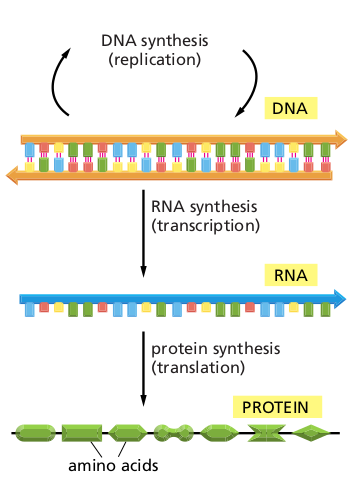
\includegraphics[width=0.5\textwidth]{TranslationAndTranscription} 
    \end{center}
    \caption{ فرآیند رونویسی، ترجمه و مضاعف کردن}
    \label{figure:translationAndTranscription}
\end{wrapfigure}

همه سلول‌ها حاوی ماده‌ ژنتیکیِ
\lr{DNA}
هستند به طوریکه از روی بخش‌هایی از این ماده ژنتیکی در فرآیند رونویسی
\footnote{\lr{transcription}}
مولکول
\lr{RNA}
ساخته می‌شود. در واقع کد ذخیره شده بر روی مولکول
\lr{DNA}
به روی یک مولکول
\lr{RNA}
کپی می‌شود. در ادامه نوع خاصی از این مولکول
\lr{RNA}
به مولکول پروتئین ترجمه می‌شود. نام این فرایند، ترجمه
\footnote{\lr{translation}}
است.

 در فرآیند ساخت پروتئین از روی کد ژنتیکی، مولکول
\lr{RNA}
به عنوان واسطه عمل می‌کند علت این امر آن است که ماده ژنتیکی حساس است و نباید در دسترس همه اندامک‌ها قرار گیرد. به علاوه برای ساخت پروتئین مولکول
\lr{RNA}
وارد ریبوزوم می‌شود که این کار برای مولکول طویل
\lr{DNA}
مقدور نیست چرا مشخص نیست که کدام قسمت آن باید ترجمه شود.

در جانداران چندسلولی ماده‌ ژنتیکی تمام سلول‌ها یکسان است. در واقع در سلول‌ها ماده‌ ژنتیکی یکسان است و فقط میزان رونویسی از روی ژن‌های متفاوت فرق دارد و همین بیان متفاوت ژن‌ها شخصیت سلول را شکل میدهد. در فرآیند فوق مانند کتاب آشپزی، که خود به تنهایی کار خاصی را انجام نمی‌دهد و باید از روی آن غذا پخته شود، ماده‌ ژنتیکی نیز خود کاری در سلول انجام نمی‌دهد  بلکه باید از روی آن پرو‌تئین ساخته شود. 

\noindent
مولکول‌های پرو‌تئین دارای شکل سه بعدی هستند که رفتار سلول را کنترل می‌کنند. پروتئین‌ها کارهای مختلفی را انجام می‌دهند.

\noindent
علاوه بر ماده ژنتیکی، همه سلول‌ها دارای  غشا و سیتوپلاسم هستند.

\subsection{تمام سلول‌ها از یک جد مشترک نشات گرفته‌اند}

همان طور که در تصویر
\ref{figure:translationAndTranscription}
مشاهده می‌شود مولکول
\lr{DNA}
می‌تواند خود را مضاعف کند. سلول برای این که تکثیر پیدا کند ابتدا ماده ژنتیکی خود را مضاعف می‌کند و سپس به دو سلول دختری تقسیم می‌شود.

\noindent
در زمان مضاعف شدن ممکن است جهش‌هایی در ماده ژنتیکی ِتکثیر پیدا کرده ایجاد شود و به سلول دختری منتقل شود. این جهش‌ها به سه نوع تقسیم می‌شوند:

\begin{itemize}
\item خوب:
تغییر در جهتی است که سازگاری جاندار را با محیط افزایش می‌دهد و قدرت زیست  یا توانایی تولید مثل آن را بیشتر می‌کند.
\item بد:
تغییر باعث کاهش قدرت زیست یا تولید مثل جاندار می‌شود.
\item خنثی:
تغییری در قدرت زیست و تولید مثل ایجاد نمی‌شود.
\end{itemize}

تکامل فرآیندی است که طی آن گونه‌های با سازگاری کمتر تغییر کرده و گونه‌های با سازگاری بیشتر را به وجود می‌آوردند و این گونه‌ها به دلیل داشتن ویژگی‌های زیستی سازگارتر جایگزین گونه قبلی می‌شوند .
اساس تغییر در گونه‌ها از یک نسل به نسل بعد تغییر ماده ژنتیکی آن‌ها است  که به آن جهش گفته می‌شود. این جهش‌ها در تولید‌مثل‌های جنسی پیچیدگی بیشتری دارند.

\bigskip
به طور کلی سلول‌ها به دو دسته کلی تقسیم می‌شوند:
\begin{itemize}
\item پروکاریوت‌ها 
\footnote{\lr{Prokaryote}}
\item یوکاریوت‌ها
\footnote{\lr{Eukaryote}}
\end{itemize}

\subsection{سلول پروکاریوتی\protect\footnote{\lr{Eukaryotic cell}}}

\begin{wrapfigure}[17]{l}{0.6\textwidth}
	\centering
	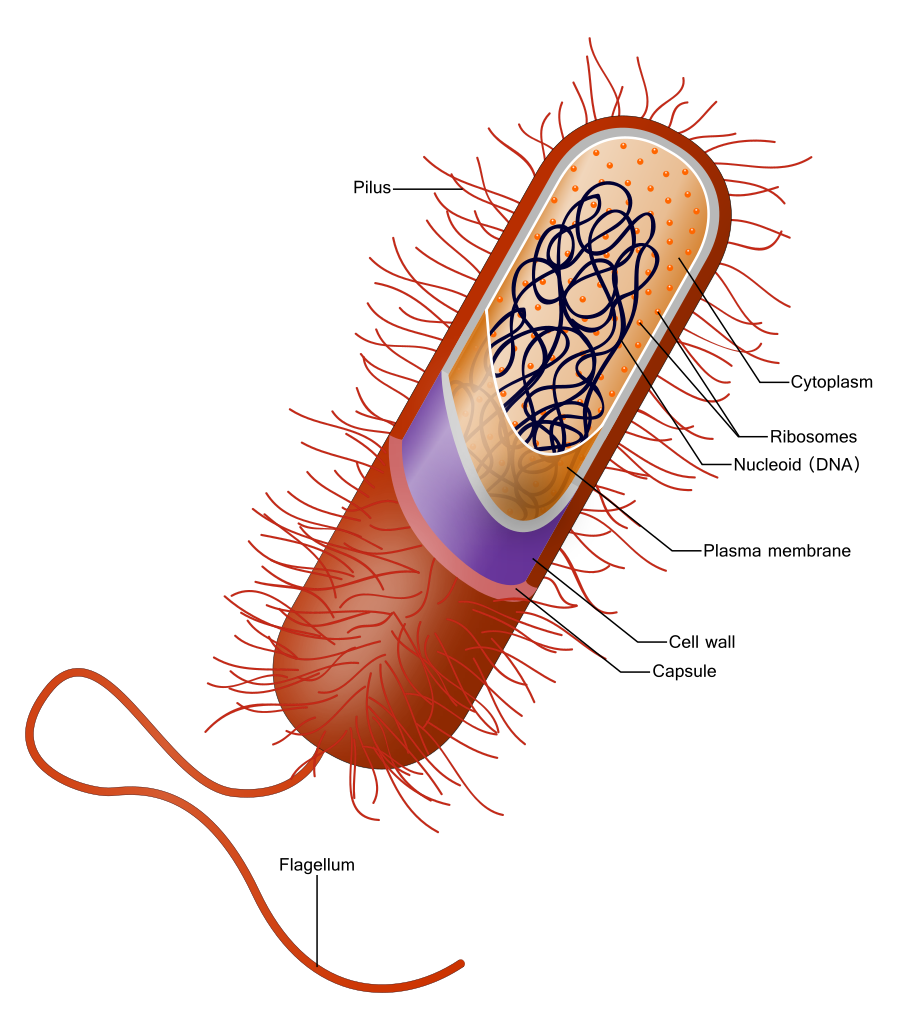
\includegraphics[width = 0.6\textwidth]{Prokaryote_cell}
\end{wrapfigure}

پروکاریوت به معنی پیش از هسته است و به این موضوع اشاره دارد که پروکاریوت‌ها فاقد هسته هستند و ماده ژنتیکی آن‌ها درون سیتوپلاسم حضور دارد. افراد این گونه عموما تک‌سلولی هستند اما در مواردی به صورت زنجیره به هم پیوسته در کنار یکدیگر زندگی می‌کنند. 

پروکاریوت‌ها شکل و ساختار ساده‌ای دارند با این حال از نظر شیمیایی متنوع‌ترین و خلاق‌ترین گونه جانداران هستند به طوریکه در طیف وسیعی از زیستگاه‌ها قدرت زندگی دارند.

\noindent
سلول پروکاریوتی در مدت زمان کمتر از 20 دقیقه می‌تواند تکثیر شود، در نتیجه درحدود 11 ساعت می‌تواند بیشتر از هشت میلیارد از خود تکثیر کند یعنی عددی بیشتر از تعداد انسان‌ها روی کره زمین!

\noindent
طبق سیستم ‌سه ‌دسته‌ای
\footnote{\lr{Three-domain system}}
پروکاریوت‌ها به دو دسته زیر تقسیم می‌شوند:

\begin{itemize}
\item باکتری (یوباکتری)
\footnote{\lr{Bacteria}}
\item آرکئا (آرکی باکتری) 
\footnote{\lr{Archaea}}
	\begin{itemize}
	\item
	می‌توانند در جاهایی زندگی کنند که اکثر سلول ها قدرت زندگی ندارد مثلا چشمه های اتشفشانی یا قطب جنوب.
	\item
	به نظر می رسد که این گونه میل به زندگی در مناطقی را دارد که مشابه با شرایط اولیه کره زمین است. 	
	\end{itemize}
\end{itemize}

\subsection{سلول یوکاریوتی\protect\footnote{\lr{Eukaryotic cell}}}

یوکاریوت به معنی خوش‌هسته است و به این اشاره دارد که این نوع از سلول‌ها دارای هسته هستند. علاوه بر این سلول‌های یوکاریوتی دارای اندامک
\footnote{\lr{Organelle}}
هستند
سلول‌های یوکایوتی عموما بزرگتر از سلول‌های پروکاریوتی هستند.
همانطور که در شکل
\ref{figure:KindsOfCell}
مشاهده می‌شود جاندارانِ یوکاریوتی به دو دسته چند‌سلولی و تک‌سلولی تقسیم می‌شوند.
\pagebreak

\begin{figure}[h]
\begin{center}
\begin{tikzpicture}
\path[mindmap,concept color=black!65!white,text=white]
node[concept] {\rl{{\Large \em انواع گونه‌ها}}}
[clockwise from=-60]
child[concept color=black!70!white] {
	node[concept] {\rl{پروکاریوتی}}
	[clockwise from=60]
	child[concept color=black!75!white]
	{ node[concept] {\rl{باکتری}} }
	child[concept color=black!75!white] 
	{ node[concept] {\rl{آرکئا} }}
}
child[concept color=black!70!white] {
	node[concept] {\rl{یوکاریوتی}}
	[clockwise from=-180]
	child [concept color=black!75!white]{ 
	node[concept] {\rl{تک‌سلولی} }
		child[concept color=black!80!white]
		{ node[concept] {\rl{آمیب‌ها} }}
		child[concept color=black!80!white] 
		{ node[concept] {\rl{مخمر‌ها} }}
	}
	child [concept color=black!75!white]{ 
	node[concept] {\rl{چندسلولی} }
		child[concept color=black!80!white]
		{ node[concept] {\rl{گیاهان} }}
		child[concept color=black!80!white]
		{ node[concept] {\rl{جانوران} }}
		child[concept color=black!80!white]
		{ node[concept] {\rl{قارچ‌ها} }}
	}
}
;
\end{tikzpicture}
\end{center}
\caption{تقسیم‌بندی انواع جانداران}
\label{figure:KindsOfCell}
\end{figure}

~\pagebreak
\subsection{تفاوت بین سلول یوکاریوتی و پروکاریوتی}

در جدول
\ref{table:difBetweenProAndEu}
برخی از تفاوت‌ها بین سلول‌های یوکاریوتی و پروکاریوتی ذکر شده است:

\begin{table}[h]
	\centering
	\begin{tabular}{|c|c|}
	\hline
سلول پروکاریوتی	& سلول یوکاریوتی
	\\
	\hline
اندازه سلول کوچک است
($ > 5 \mu m $)
&
اندازه سلول بزرگ است
($ <10 \mu m $)
	\\
	\hline
به صورت تک سلولی
	&
به صورت چند سلولی
	\\
	\hline
بدون هسته هستند و اندامک غشاءداری مانند میتوکندری ندارند
&
هسته و اندامک‌های غشاء دار دارند
	\\
	\hline
\lr{DNA}
به صورت حلقوی است و پروتئینی به همراه ندارد
&
 \lr{DNA}
 به صورت خطی است و به همراه پروتئین‌هایی ساختار کروماتین را میسازد
	\\
	\hline
ریبوزوم‌ها کوچک هستند
($ 70S $)
&
ریبوزوم‌ها بزرگ هستند
($ 80S $)
	\\
	\hline
اسکلت سلولی ندارند ؟
& 
اسکلت سلولی دارند
	\\
	\hline
تحرک توسط تاژک
\footnote{\lr{flagellum}}
 چرخان سفت و سخت (ساخته شده از فلاژلین
\footnote{\lr{Flagellin)}} 
 )
 &
 تحرک توسط تاژک یا مژک
 \footnote{\lr{Cilia}}
 انعطاف‌پذیر و موج‌زن ( ساخته شده توسط توبولین
 \footnote{\lr{Tubulin}}
 )
	\\
	\hline
تقسیم سلولی با شکافت دوتایی
\footnote{\lr{Binary fission}}
&
تقسیم سلولی با میوز
\footnote{\lr{Meiosis}}
یا میتوز
\footnote{\lr{Mitosis}}
	\\
	\hline
مضاعف‌شدن
\footnote{Reproduction}
همیشه به صورت غیر جنسی است
&
مضاعف شدن به صورت جنسی یا غیرجنسی است
	\\
	\hline
تنوع بسیار زیاد در مسیر‌های متابولیکی
\footnote{\lr{Metabolic pathway}}
&
مسیر‌های متابولیک مشترک
	\\
	\hline												
	\end{tabular}
	\caption{ تفاوت انواع سلول}
	\label{table:difBetweenProAndEu}
\end{table}


\subsection{سیستم غشائی درونی}

\begin{wrapfigure}[12]{l}{0.6\textwidth}
	\centering
	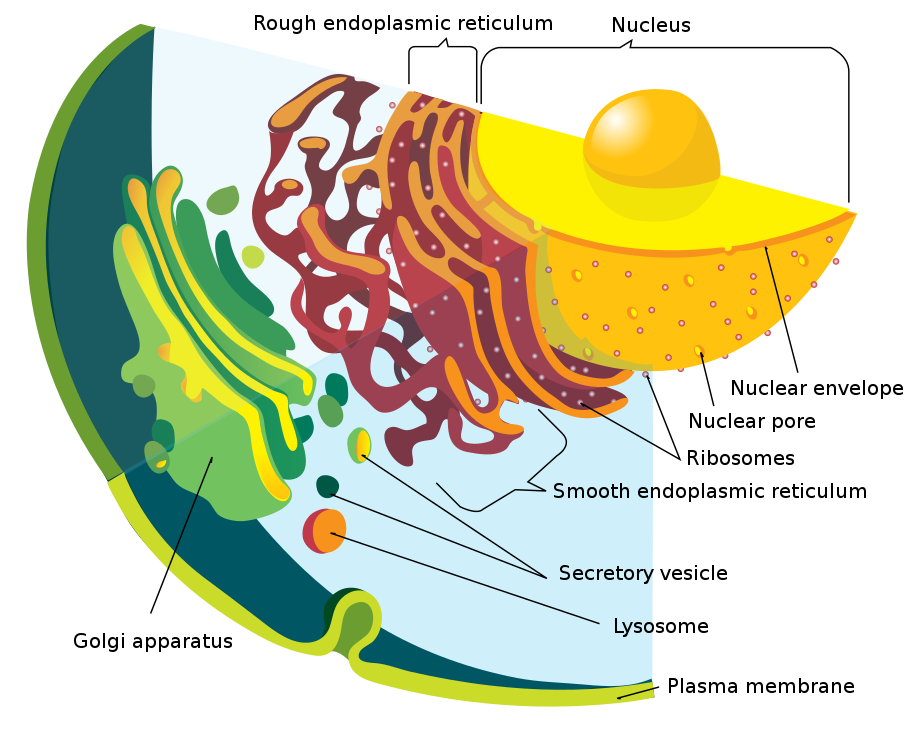
\includegraphics[width=0.6\textwidth]{Eukaryotic_cell}
	\caption{سیستم غشائی درونی}
	\label{figure:endomembraneSystem}
\end{wrapfigure}

سلول‌های یوکاریوتی شامل تعدادی ساختار غشاء‌دار
\footnote{\lr{Membrane-bound structure}}
هستند که به مجموع این ساختار‌ها، دستگاه غشائی درونی
\footnote{\lr{Endomembrane system}}
گفته می‌شود. در شکل
\ref{figure:endomembraneSystem}
اجزاء این دستگاه را مشاهده می‌کنیم. محفظه‌های
\footnote{\lr{Compartment}}
ساده مانند وزیکول
\footnote{\lr{Vesicle}}
و واکوئل
\footnote{\lr{Vacuole}}
می‌توانند با جوانه زدن بقیه غشاء‌ها به وجود بیایند.

عمدتا تغذیه سلول به وسیله فرآیند اندوسیتوز
\footnote{\lr{Endocytosis}}
انجام می‌شود. همان طور که در شکل
\ref{figure:Endocytosis}
مشاهده می‌کنید غذا توسط غشاء سلول بسته بندی و وارد سلول می‌شود.
این بسته‌بندی به صورت وزیکول و یا واکوئل است.
همچنین سلول‌ها می‌توانند موادی را که تولید می‌کنند با فرآیند اگزوسیتوز
\footnote{\lr{Exocytosis}}
به خارج از سلول ارسال کنند.

\pagebreak
\begin{figure}[t]
	\centering

	\subfloat[وزیکول]{{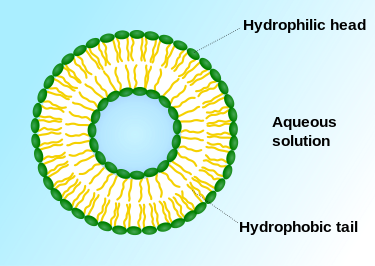
\includegraphics[width=5cm]{Vesicle} }}
    \qquad
    \subfloat[واکوئل]{{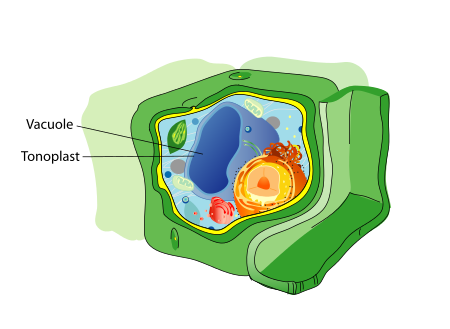
\includegraphics[width=5cm]{Vacuole} }}
    	\bigskip
	
	\begin{subfigure}[b]{0.85\textwidth}
		\centering
		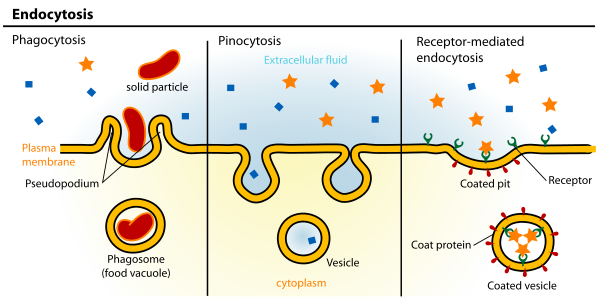
\includegraphics[width=0.8\textwidth]{Endocytosis}
		\caption{انواع اندوسیتوز}
		\label{figure:Endocytosis}
	\end{subfigure}	
	\caption{سیستم غشائی درونی}
\end{figure} 

~

\pagebreak
\subsection{اندامک‌ها\protect\footnote{\lr{Organelle}}}

\begin{figure}[t]
	\centering
	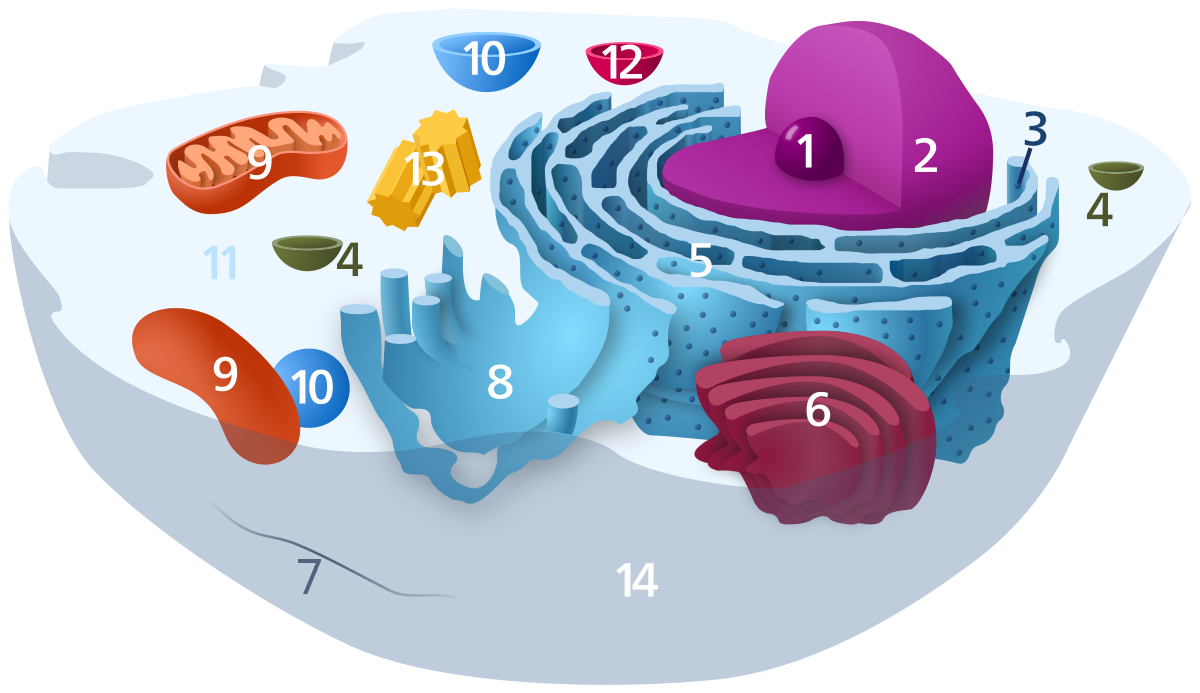
\includegraphics[width=0.5\textwidth]{Animal_cell}
	\caption{ اندامک‌های یک سلول جانوری.
	\lr{1.Nucleolus}
	\lr{2.Nucleus}
	\lr{3.Ribosome}
	\lr{4.Vesicle}
	\lr{5.Rough endoplasmic reticulum}
	\lr{6.Golgi apparatus}
	\lr{7.Cytoskeleton}
	\lr{8.Smooth endoplasmic reticulum}
	\lr{9.Mitochondrion}
	\lr{10.Vacuole}
	\lr{11.Cytosol }
	\lr{12.Lysosome}
	\lr{13.Centrosome}
	\lr{14.Cell membrane}	
	}
	\label{figure:Organelle}
\end{figure}

اندامک‌ها اجزائی هستند که وظایفی را به عهده دارند.  در زیر بعضی از آنها به اختصار توضیح داده شده‌اند:

\begin{description}
\item[\lr{Golgi apparatus}]
گلژی وظیفه ارسال پروتئین‌های جدید به جایگاه‌های مناسب را بر عهده دارد.
شکل
\ref{figure:Organelle}
(۶)
\item[\lr{Lysosome}]
لیزوزوم مواد غیرلازم را تجزیه می‌کند.
شکل
\ref{figure:Organelle}
(12)
\item[\lr{Cytosol }]
مایعی که سایر اندامک‌ها در آن جای دارند.
\ref{figure:Organelle}
شکل
(11)
\item[\lr{Cytoskeleton}]
اسکلت سلولی مانند اسکلت بدن برای سلول است و اندامک‌ها را در جایگاه مناسب نگاه می‌دارد. اسکلت سلولی تنها از یک بخش تشکیل نشده و اجزاء مختلفی در کنار هم قرار گرفته‌اند تا آن را تشکیل دهند.
شکل
\ref{figure:Organelle}
(7)

اسکلت سلولی یوکاریوت‌ها از سه نوع فیلامین
\footnote{\lr{Filament}}
اصلی تشکیل شده‌اند:

\begin{itemize}
\item
میکروفلامین یا ریزرشته‌ها
\footnote{\lr{microfilament}}
 پلیمر‌هایی از پروتئین اکتین
\footnote{\lr{Actin}}
هستند که باریک می‌باشند و هفت نانومتر قطر دارند.
\item
میکروتوبول یا ریزلوله‌ها
\footnote{\lr{microtubule}}
 از پروتئین توبولین
\footnote{\lr{tubulin}}
ساخته شده‌اند و 25 نانومتر قطر دارند.
\item
رشته‌های متوسط
\footnote{\lr{intermediate filament}}
 از پروتئین‌های مختلفی ساخته شده‌اند و این برحسب سلول مورد نظر متفاوت است.
\end{itemize}

\begin{figure}[h]
	\centering
	\subfloat[ساختار میکروفلامین]{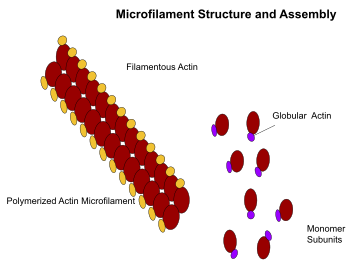
\includegraphics[width = 5cm]{Microfilament}}
	\qquad
	\subfloat[ساختار میکروتوبول]{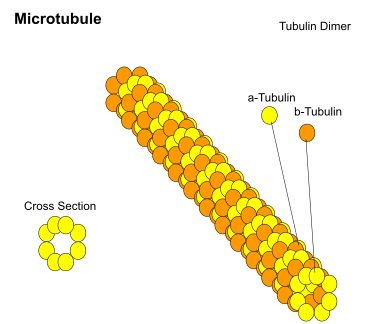
\includegraphics[width = 5cm]{Microtubule}}
\end{figure}

\begin{table}[h]
	\centering
	\begin{tabular}{|r|r|r|}
\hline
نوع اسکلت سلولی & قطر به نانومتر & ماده‌سازنده \\
\hline
میکروفیلامین & 6 & اکتین\\
فلامین متوسط & 10 & با توجه به  نوع سلول متفاوت \\
	میکروتوبول‌ & 23 & توبولین آلفا و بتا\\
\hline
	\end{tabular}
	\caption{انواع فیلامین‌های اسکلت سلولی}
\end{table}

\item[\lr{Nucleus}]

هسته در سلول‌های یوکاریوتی یافت می‌شود . اغلب، سلول‌ها یک هسته دارند اما سلول‌های وجود دارند که هسته ندارند و یا بیش از یک هسته دارند.
شکل
\ref{figure:Organelle}
(2)

 هسته را پوشش هسته
\footnote{\lr{Nuclear envelop}}
فرا گرفته‌است که این پوشش از دو لایه تشکیل شده است.

\begin{figure}[h]
	\centering
	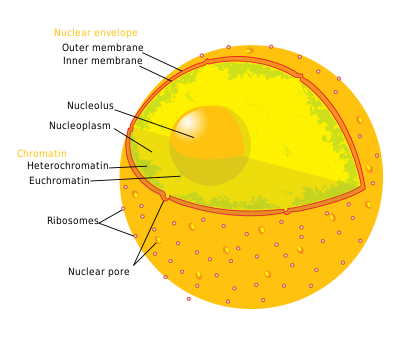
\includegraphics[width=0.4\textwidth]{Nucleus}
\end{figure}

ماده ژنتیکی
(\lr{DNA})
درون هسته قرار دارد.  در شرایط خاص به این ماده ژنتیکی کروموزوم
\footnote{\lr{Chromosome}}
،کروماتین
\footnote{\lr{Chromatin}}
و یا کروماتید
\footnote{\lr{Chromatid}}
گفته می‌شود.
وقتی که سلول در حال تقسیم نیست،	
\lr{nuclear DNA}
به همراه انواعی از پروتئین‌ها به صورت کروماتین شکل میگیرند. سپس هنگامی که سلول می‌خواهد تقسیم انجام دهد، کروماتین به صورت ساختار فشرده‌ی کروموزوم در  می‌آید.

\begin{figure}[htbp]
	\centering
	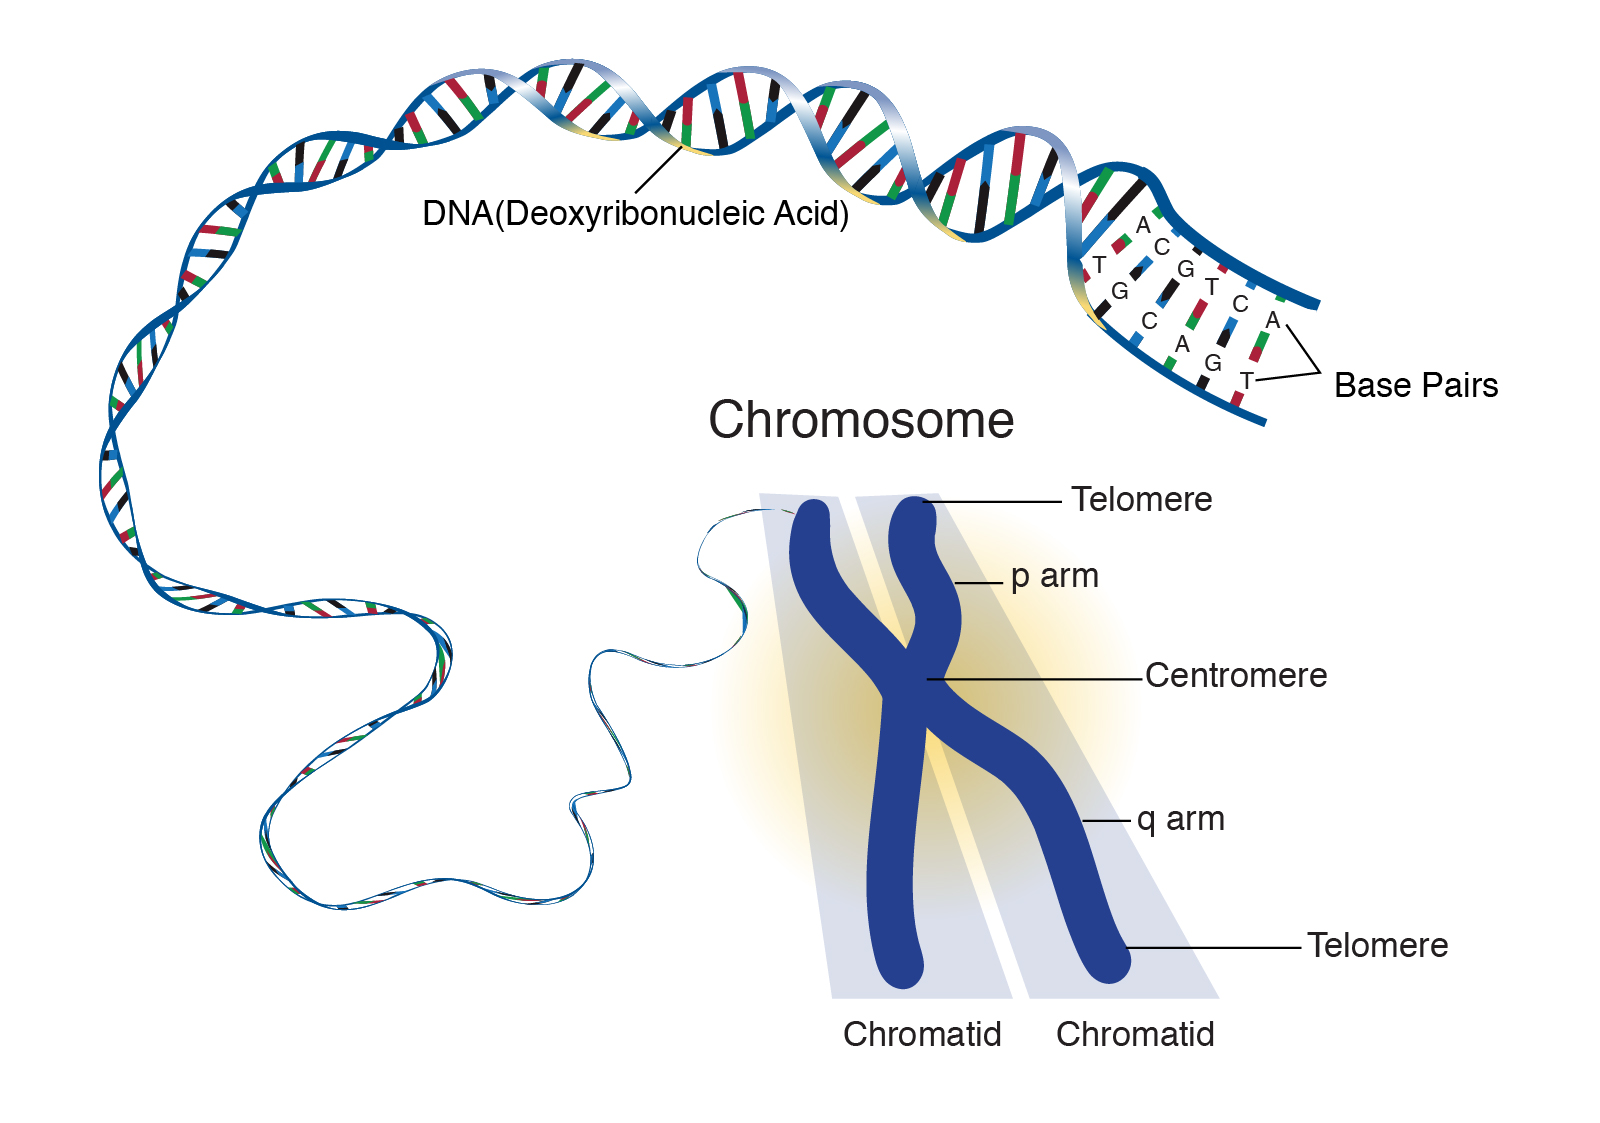
\includegraphics[width=0.7\textwidth]{Chromosome}
	\caption{ساختار کروموزوم}
	\label{figure:Chromosome}
\end{figure}

همانطور که در شکل
\ref{figure:Chromosome}
مشاهده می‌کنید کروموزوم از دو قسمت
\lr{P-arm}
و
\lr{Q-arm}
ساخته شدند که اولی بازوی کوتاه و دومی بازوی بلند کروموزوم را تشکیل می‌دهند.

\item[\lr{Mitochondria}]
این اندامک خود دارای
\lr{DNA}
است و دو لایه غشاء دارد. میتوکندری وظیفه تولید انرژی شیمیایی برای سلول را برعهده دارد. طی این فرآیند میتوکندری قند یا چربی را اکسید می‌کند و
\lr{ATP}
را به عنوان انرژی شیمیایی آزاد می‌کند.
شکل
\ref{figure:Organelle}
(9)

\item[\lr{Chloroplast}]
کلروپلاست در گیاهان وجود دارد. و سلول‌های گیاهی انرژی خود را از طریق این اندامک تامین می‌کنند. کلروپلاست دارای کلروفیل
\footnote{\lr{Chlorophyll}}
می‌باشد. کلروفیل نور خورشید را به دام می‌اندازد و آن را در ملکول‌های
\lr{ATP}
و
\lr{NADPH}
ذخیره می‌کند. در کنار این فرآیند اکسیژن آزاد می‌شود و در نتیجه میتوکندری می‌تواند از آن استفاده کند.

\item[\lr{Endoplasmic reticulum}]
شبکه آندومپلاسمی از دو قسمت نرم
\footnote{\lr{Smooth endoplasmic reticulum}}
و سخت
\footnote{\lr{Rough endoplasmic reticulum}}
تشکیل شده است. شکل
\ref{figure:Organelle}
(5 و 8).
بر روی شبکه آندوپلاسمی زبر تعدادی ریبوزوم  وجود دارد که این ریبوزوم‌ها از روی 
\lr{RNA}
ها پروتئین می‌سازند. هنگامی که این پروتئین‌ها ساخته می‌شوند به وسیله شبکه آندوپلاسمی زبر به سمت گلژی فرستاده می‌شوند.
 شبکه آندوپلاسمی نرم نیز محصولاتی مانند لیپید و یا فسفولیپید تولید می‌کند.
 
\begin{figure}[htbp]
	\centering
	\subfloat[ساختار میتوکندری]{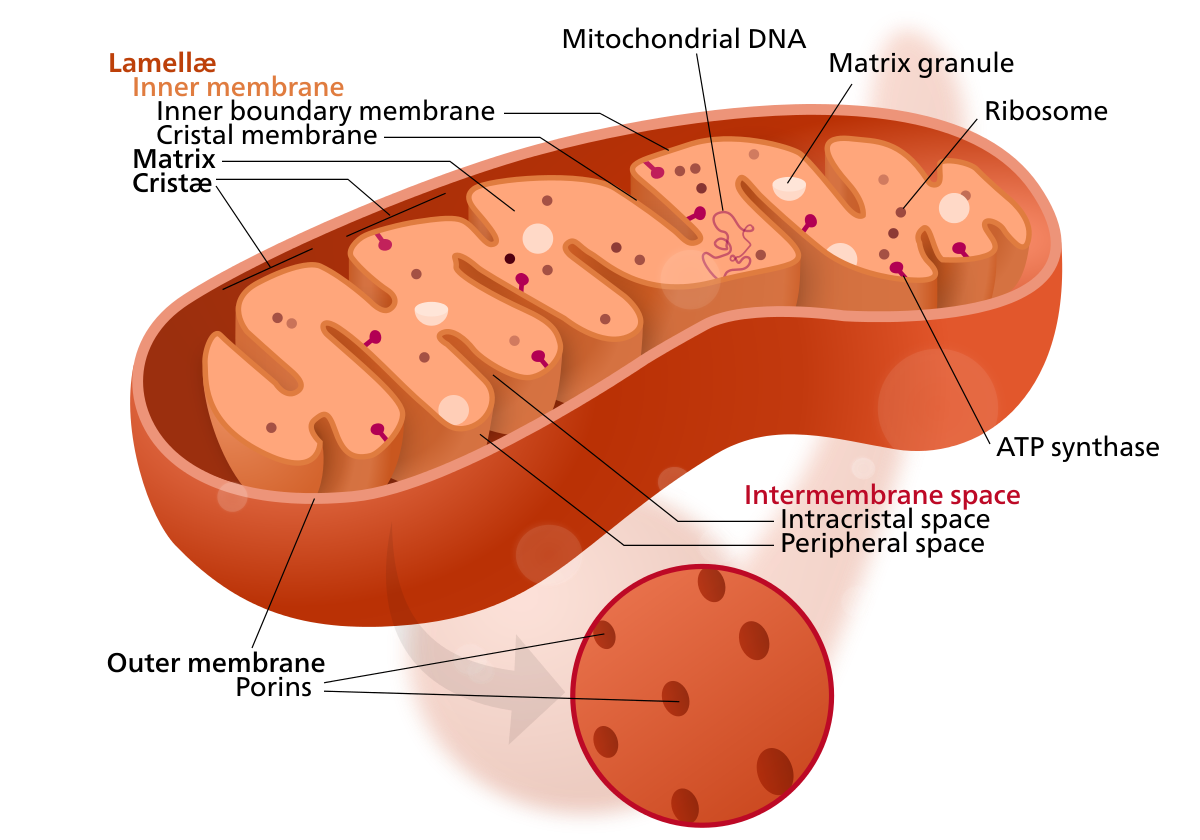
\includegraphics[width=7cm]{Mitochondrion_structure}}
	\qquad
	\subfloat[ساختار کلروپلاست]{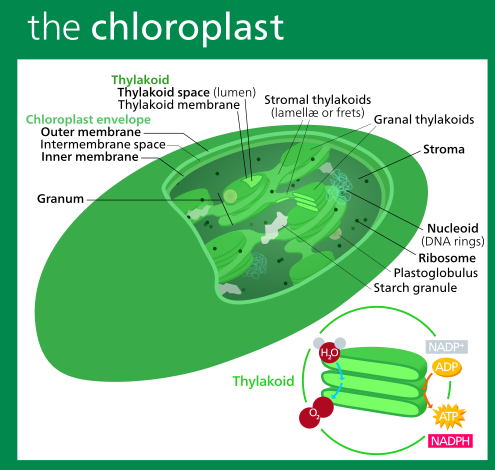
\includegraphics[width=7cm]{Chloroplast}}
\end{figure} 
 
\begin{figure}[t]
	\floatbox[{\capbeside\thisfloatsetup{capbesideposition={right,top},capbesidewidth=6cm}}]{figure}[\FBwidth]
{\caption
{
\lr{1.Nucleus}
\lr{2.Nuclear~pore}
\lr{3.Rough~endoplasmic~reticulum~(RTE)}
\lr{4.Smooth~endoplasmic~reticulum~(SER)}
\lr{5.Ribosome~on~rough~ER}
\lr{6.Proteins~that~are~transported}
\lr{7.Trasport~vesicle}
\lr{8.Golgi~apparatus}
\lr{9.Cis~face~of~Golgi~apparatus}
\lr{10.Trans~face~of~Golgi~apparatus}
\lr{11.Cisternae~of~the~Golgi~apparatus}
}
\label{fig:EndoplasmicReticulum}}
{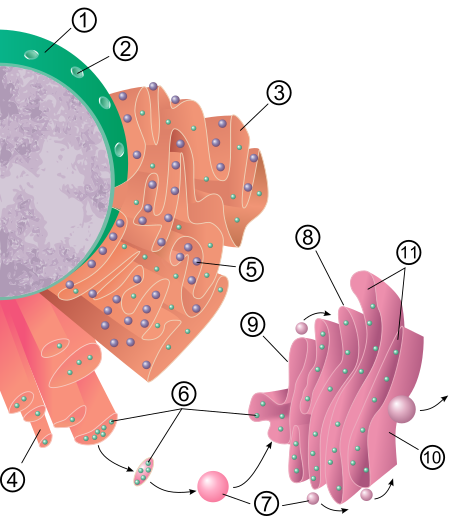
\includegraphics[width=0.4\textwidth]{Endoplasmic_reticulum_golgi}}

\end{figure}  
 
\end{description}

\pagebreak
\subsection{کلروپلاست و میتوکندری شباهت زیادی به باکتری دارند}

همانطور که مشاهده شد این دو اندامک شباهت زیادی به باکتری‌ها دارند و نظریه‌ای و جود دارد که طی آن سلول یوکاریوتی این دو اندامک را به صورت غذا وارد خود ساخته و سپس با آن همزیست شده است. به شکل
\ref{figure:PrimaryEndosymbiosis}
رجوع کنید.

\begin{figure}[hbt]
	\centering
	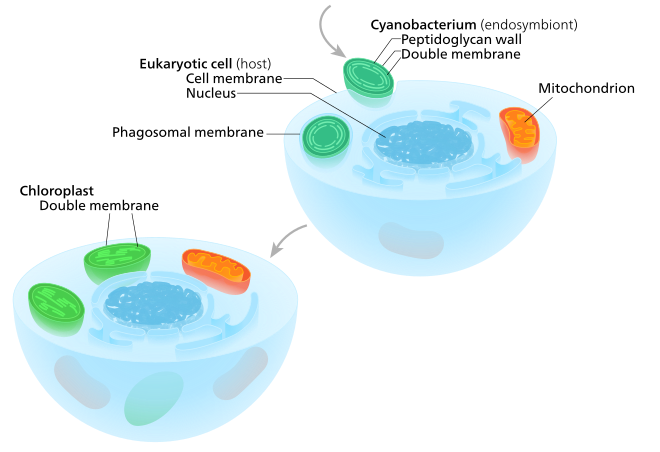
\includegraphics[width = 0.6\textwidth]{Chloroplast_endosymbiosis}
	\caption{\lr{A eukaryote with mitochondria engulfed a cyanobacterium in an event of serial primary endosymbiosis, creating a lineage of cells with both organelles.}}
	\label{figure:PrimaryEndosymbiosis}
\end{figure}

\subsection{موجودات مدل}
در زیست شناسی نمونه‌های خاصی وجود دارد که سایر گونه‌ها شباهت زیادی به آن‌ها دارند در نتیجه زیست شناسان ابتدا روی این گونه‌ها آزمایش می‌کنند. در زیر به مواردی اشاره شده است:

\begin{itemize}
\item ای کولی
\item ساکارومایسس
\item آرابیدوبسیس
\item مگس
\item کرم
\item ماهی
\item موش
\item انسان
\end{itemize}

\pagebreak
\subsection{نوکلئیک اسید‌ها}

\begin{wrapfigure}{l}{8cm}
	\centering
	
	\begin{subfigure}[b]{8cm}
		\centering
		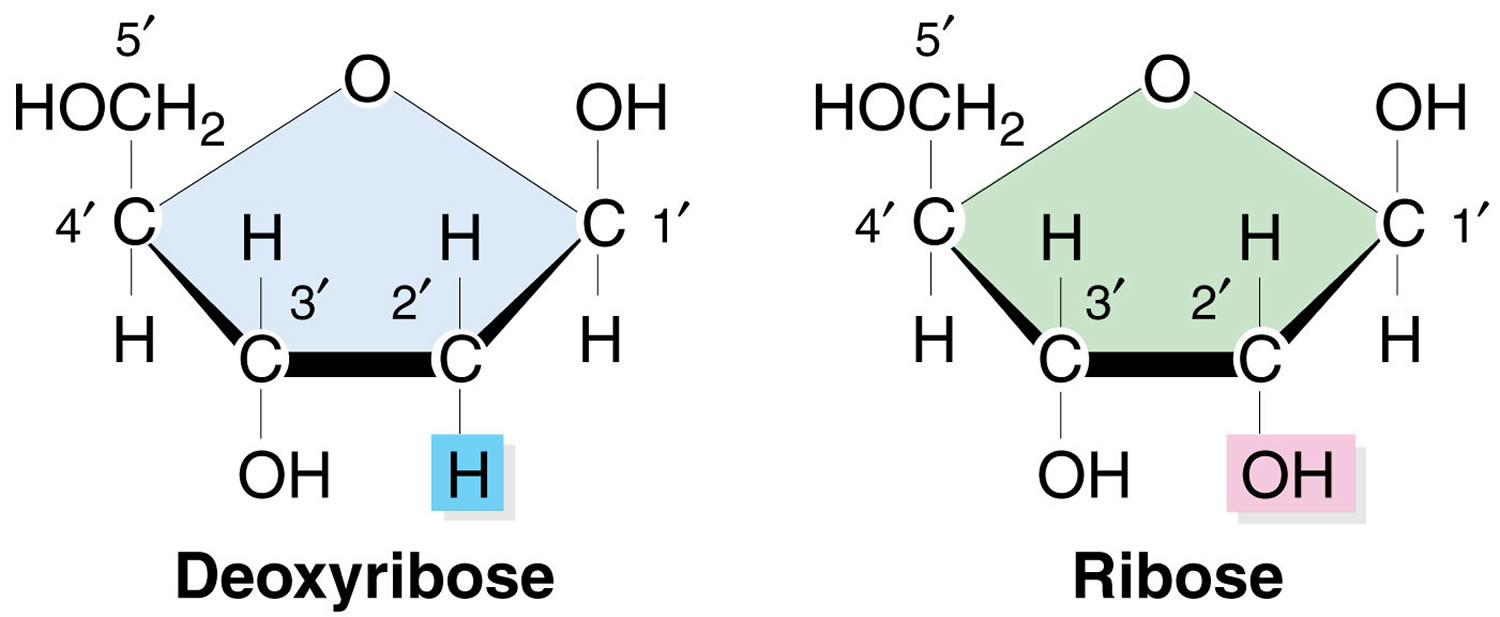
\includegraphics[width = 7cm]{Ribose_and_deoxyribose}
		\caption{قند ریبوز و دئوکسی‌ریبوز}	
	\end{subfigure}
	\begin{subfigure}[b]{8cm}
		\centering
		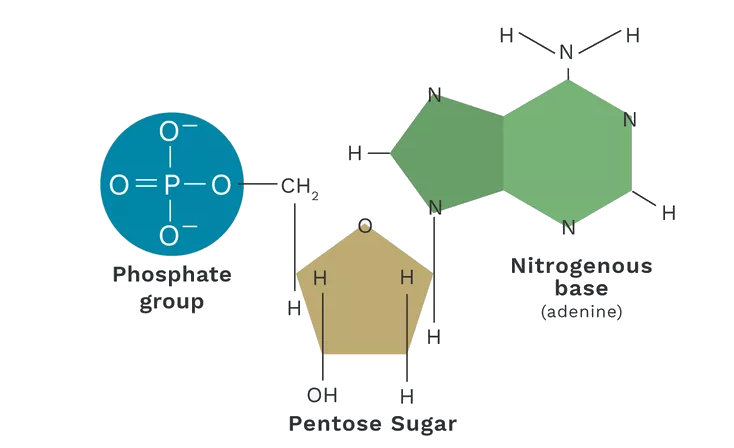
\includegraphics[width=8cm]{Nucleotide}
		\caption{اجزاء ریزملکول نوکلئوتید}
		\label{figure:Nucleotide}
	\end{subfigure}
	
\end{wrapfigure}

در سال 1870 فردریک میشر از هسته سلول، ماده ای استخراج کرد که خاصیت اسیدی داشت به همین علت نام آن را نوکلئیک اسید
\footnote{\lr{Nucleic acid}}
به معنی اسید هسته‌ای گذاشت. بعد‌ها مشخص شد که نوکلئیک اسید‌ها دو نوع هستند:
\begin{itemize}
\item ریبو نوکلئیک اسید یا 
\lr{RNA}
که در ساختار آن قند ریبوز
\footnote{\lr{Ribose}}
 به کار رفته است.
\item دئوکسی ریبو نوکلئیک اسید یا
\lr{DNA}
که در ساختار آن قند دئوکسی ریبوز
\footnote{\lr{Deoxyribose}}
 به کار رفته است.
\end{itemize}

نوکلئیک اسید‌ها همانند پروتئین‌ها و کربوهیدرات‌ها پلی‌مر هستند. واحد‌ مونومری نوکلئیک اسید‌ها، نوکلئوتید
\footnote{\lr{Nucleotide}}
است.
همانطور که در شکل
\ref{figure:Nucleotide}
مشاهده می‌کنید، مولکول نوکلئوتید از سه بخش تشکیل شده است:
\begin{itemize}
\item  یک تا سه گروه فسفات
\item  قند پنتوز که ریبوز در
\lr{RNA}
و
دئوکسی ریبوز در
\lr{DNA}
است
\item  باز آلی نیتروژن‌دار
\end{itemize}

در تمام انواع این مولکول قسمت فسفات و قند یکسان است (با توجه به دی‌ان‌ای یا آرآن‌ای بودن) اما با توجه به نوع باز پنج نوع مولکول نوکلئوتید به وجود می‌آیند که در نوکلئیک‌اسید‌ها
به کار رفته است:
\begin{itemize}
\item پورین‌ها با دو حلقه
\footnote{\lr{Purine}}
	\begin{itemize}
	\item آدنین
	\footnote{\lr{Adenine (A)}}
	\item گوانین
	\footnote{\lr{Guanine (G)}}
	\end{itemize}
\item پریمیدین‌ها با یک حلقه
\footnote{\lr{Pyrimidine}}
	\begin{itemize}
	\item سیتوزین
	\footnote{\lr{Cytosine (C)}}
	\item تیمین
	\footnote{\lr{Thymine (T)}}
	در دئوکسی ریبونوکلئیک اسید	
	\item یوراسیل
	\footnote{\lr{Uracil (U)}}
در ریبونوکلئیک اسید
	\end{itemize}
\end{itemize}

\noindent
در شکل
\ref{figure:bases}
ساختار این باز‌ها مشخص شده است.

\begin{figure}[ht]
	\centering
	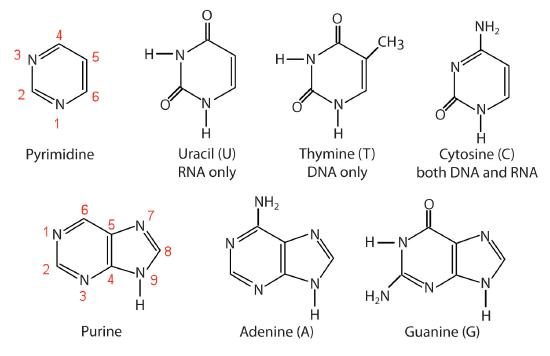
\includegraphics[width = 10cm]{Bases}
	\caption{انواع باز‌هایی که در مولکول
	\lr{DNA}
	و
	\lr{RNA}
	به کار رفته است.	
	}
	 \label{figure:bases}
\end{figure}

از کنار هم قرار گرفتن مولکول‌های نوکلئوتید پلی‌مری خطی به وجود می‌‌آيد. اتصال بین دو مولکول نوکلئوتید از طریق برقراری پیوند کووالانسی
\footnote{\lr{Covalent}}
بین گروه فسفات یک نوکلئوتید و قند نوکلئوتید بعدی است. نوکلئوتید‌ها به صورت آزاد سه گروه فسفات دارند اما هنگام برقراری اتصال با یکدیگر دو گروه فسفات خود را از دست می‌دهند و با یک گروه فسفات در رشته پلی‌نوکلئوتیدی قرار می‌گیرند. پیوند بین دو نوکلئوتید را پیوند فسفو دی استر
\footnote{\lr{Phosphodiester bound}}
می‌نامند.

همانطور که در شکل
\ref{figure:PhosphodiesterBond}
مشاهده می‌شود در یک انتهای رشته پلی‌نوکلئوتیدی گروه فسفات وجود دارد حال آنکه در انتهای دیگر وجود ندارد به همین علت رشته پلی‌نوکلئوتیدی دارای قطبیت است.

\pagebreak
\begin{wrapfigure}[22]{l}{9cm}
	\centering
	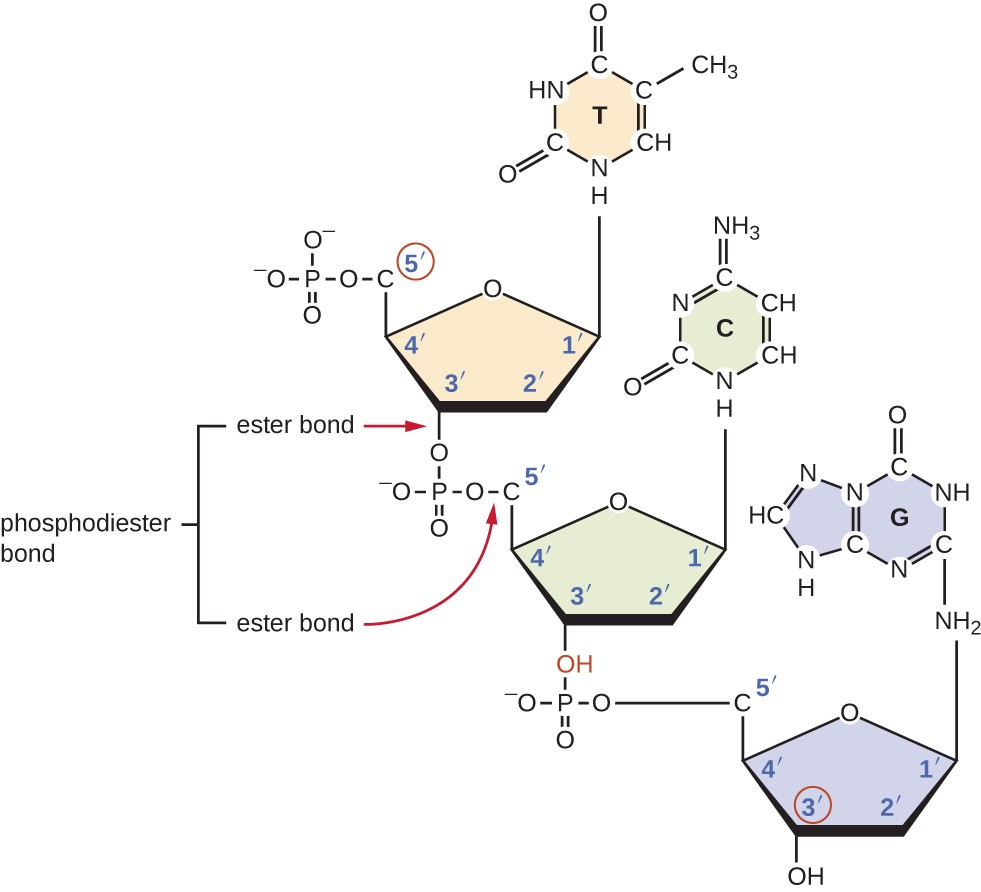
\includegraphics[width=9cm]{DNA_five_to_three}
	\caption{
	پیوند فسفودی‌استری
	\protect	
	\footnote{\lr{Phosphodiester}}
	بین  گروه فسفات متصل به کربن
	$ 5^\prime $
	یک نوکلئوتید و گروه هیدروکسیل
	\protect
	\footnote{\lr{Hydroxyl}}
	نوکلئوتید بعدی برقرار می‌شود.	
	}
	\label{figure:PhosphodiesterBond}
\end{wrapfigure}

همانطور که در شکل
\ref{figure:PhosphodiesterBond}
مشاهده می‌شود کربن
$ 5^\prime $
نوکلئوتید اول و کربن
$ 3^\prime $
نوکلئوتید آخر بیکار هستند به همین خاطر اصطلاحا می‌گویند
\lr{DNA}
از سمت
$ 5^\prime $
به سمت
$ 3^\prime $
شکل می‌گیرد.

دو رشته مولکول
\lr{DNA}
به صورت آنتی پارالل
\footnote{\lr{Antiparallel}}
در مقابل یکدیگر قرار میگیرند. در واقع یک رشته در جهت
$ 5^\prime $
به سمت
$ 3^\prime $
است و دیگری در جهت
$ 3^\prime $
به سمت
$ 5^\prime $
.

پیوند بین دو رشته از نوع هیدروژنی است. هر باز فقط با مکمل خود پیوند برقرار می‌کند به این صورت که آدنین مکمل تیمین است و سیتوزین مکمل گوآنین. گاهی گوانین نیز با تیمین مکمل می‌شود اما این جفت یک پیوند هیدروژنی برقرار می‌کند و پایداری کمی دارد.
بین آدنین و تیمین دو پیوند هیدروژنی شکل می‌گیرد و بین سیتوزین و گوآنین سه پیوند. این نکته در کار‌های محاسباتی اهمیت دارد.
به یک جفت باز که با هم پیوند هیدروژنی تشکیل می‌دهند 'جفت باز` 
\footnote{\lr{Base pair}}
گفته می‌شود.

باز‌هایی که مکمل هم هستند هنگامی که کنار هم قرار میگیرند فاصله یکسانی را میسازند که این باعث استحام نردبان
\lr{DNA}
می‌شود حال آنکه اگر دو باز که مکمل هم نیستند در کنار یکدیگر قرار بگیرند فاصله‌ای که می‌سازند با سایر جفت بازها متفاوت است و استحام مولکول
\lr{DNA}
از بین می‌رود.

هنگامی که در مولکول
\lr{DNA}
جفت بازها کنار یکدیگر قرار می‌گیرند به هم فشار می‌آورند و الکترون تبادل می‌کنند که به آن
\lr{`Base stacking'}
گفته می‌شود.

\pagebreak
\subsubsection{مولکول دی ان ای}
مولکول
\lr{DNA}
به صورت دورشته‌ای
\footnote{\lr{Double stranded}}
است. به نظر می‌رسد که طبیعت برای این که از تغییر ماده‌ژنتیکی هنگام تولید مثل جلوگیری کند تصمیم گرفته است تا این مولکول به صورت دورشته‌ای باشد چرا که از روی یک رشته می‌توان رشته دیگر را ترمیم کرد.

\begin{figure}[h]
	\centering
	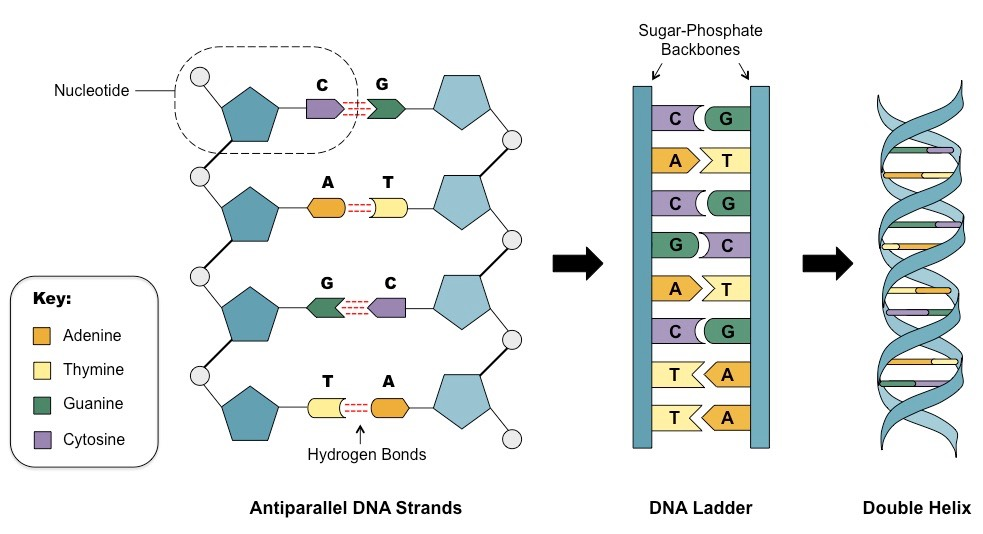
\includegraphics[width=11cm]{double-stranded-dna}
\end{figure}

ساختار مولکول
\lr{DNA}
به صورت پیچشی است و پیچ‌های مولکول، اهمیت زیادی دارد و با توجه به نوع این پیچش‌ها مولکول فرم‌های متفاوتی پیدا می‌کند.
همان طور که در شکل
\ref{figure:majorAndMinorGroove}
مشاهده می‌کنید ساختار پیچشی مولکول
\lr{DNA}
شیار‌هایي را به وجود می‌آورد. این شیار‌ها به دو دسته شیار اصلی
\footnote{\lr{Major groove}}
و شیار فرعی
\footnote{\lr{Minor groove}}
تقسیم می‌شوند. اهمیت این شیارها در این است که احتمال ساخت پروتئین از روی آن‌ها بیشتر است و به اصطلاح
\lr{Binding site}
به وجود می‌آورند.

\begin{figure}[h]
	\centering
	\subfloat[]{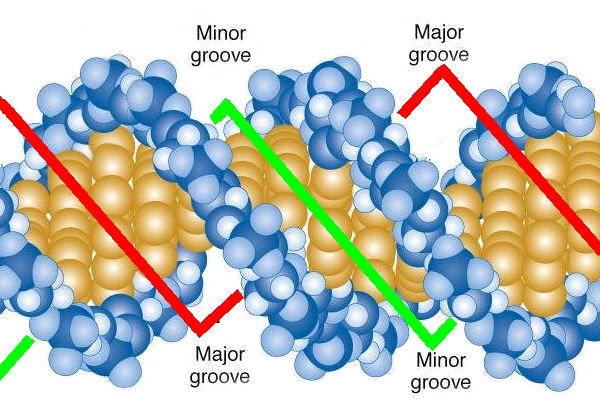
\includegraphics[width=6cm]{major_and_minor_groove_first}}
	\subfloat[]{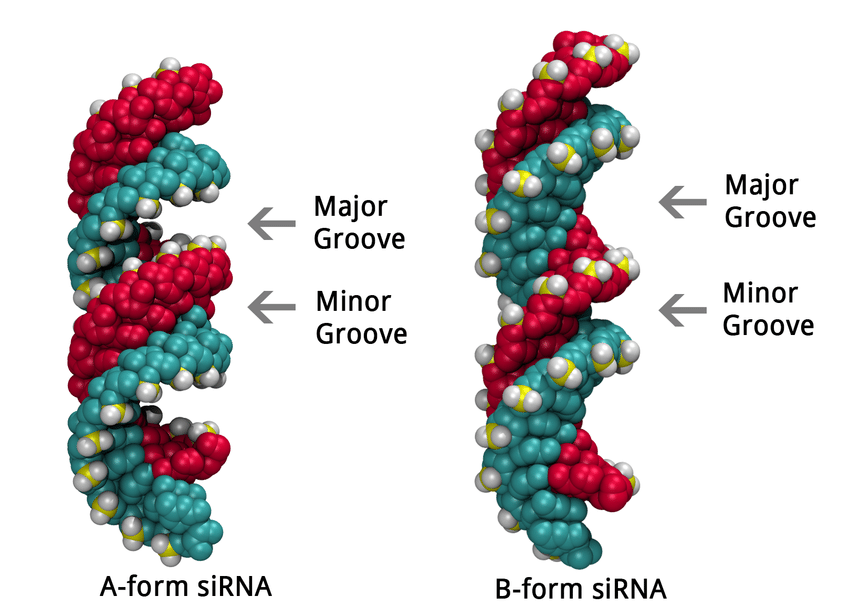
\includegraphics[width=8cm]{major_and_minor_groove_second}}	
	\caption{شیار اصلی و فرعی در مولکول
	\lr{DNA}}
	\label{figure:majorAndMinorGroove}
\end{figure}

فرض کنید که از روی توالی
\lr{ATTA}
پروتئین خاصی ساخته می‌شود و ما می‌خواهیم توالی‌هایی از
\lr{DNA}
که به این صورت است را پیدا کنیم. در چنین موقعی باید به این نکته توجه کنیم که توالی‌های بر روی شیار اصلی و فرعی مهم‌تر هستند و احتمال ساخت پروتئین از روی آنها بیشتر است در نتیجه باید به ساختار سه بعدی مولکول
\lr{DNA}
نیز توجه کنیم. همچنین شیار‌های اصلی در مقایسه با شیار فرعی بیشتر در معرض رونویسی هستند.

\pagebreak
\subsubsection{مولکول آر ان ای}
همانطور که قبلا گفته شد
\lr{RNA}
یک نوع
\lr{nucleic acid}
و یا همان اسید هسته‌ای است که به علت داشتن قند ریبوز به آن
\lr{ribonucleic acid}
گفته می‌شود. در گذشته تصور می‌شد تنها کاری که مولکول
\lr{RNA}
انجام می‌دهد، رونویسی از مولکول
\lr{DNA}
است اما امروزه میدانیم که
\lr{RNA}
ها ساختار سه‌بعدی مهمی دارند و کارهای عملکردی انجام می‌دهند. در واقع
\lr{RNA}
چیزی بین
\lr{DNA}
و پروتئین است. یک تئوری برای آغاز حیات در دنیا این است که حیات با مولکول
\lr{RNA}
آغاز شده است و بعد از آن این مولکول تصمیم گرفته است که
\lr{DNA}
را به وجود آورد. به این تئوری
\lr{RNA World}
گفته می‌شود.

نکته‌ای که درمورد
\lr{RNA}
وجود دارد این است که بر خلاف مولکول
\lr{DNA}
اغلب به صورت تک
\lr{Strand}
است. 
\lr{RNA}
در هسته سنتز می‌شود. بعد از سنتز
\footnote{\lr{synthesis}}
بیشتر
\lr{RNA}
ها به سیتوپلاسم مهاجرت می‌کنند. زیست‌شناسان برای آن که میزان بیان یک ژن را بسنجند میزان
\lr{RNA}
هایی که از روی آن ژن رونویسی شده است را اندازه می‌گیرند چرا که نمی‌توانند این کار را از روی پروتئین‌های مربوط به یک ژن انجام دهند. پروتئین‌ها اندکی بعد از ساخته شدن و انجام وظیفه خود، نابود می‌شوند به همین علت نمی‌توان مقدار آن‌ها را به طور دقیق اندازه گیری کرد.

\begin{table}[htbp]
	\centering
	\begin{tabular}{|c|c|}
	\hline
	\lr{DNA} & \lr{RNA} \\ \hline
	نوکلئوتید‌ها دارای قند دئوکسی ریبوز می‌باشند.
	&
	نوکلئوتید‌ها دارای قند ریبوز می‌باشند.
	\\
	\hline
	دارای نوکلئوتید تیمین می‌باشد.
	&
	دارای نوکلئوتید یوراسیل می‌باشد.
	\\
	\hline
	به صورت
	\lr{double strand}
	است.
	&
	اغلب به صورت
	\lr{single strand}
	است.
	\\
	\hline
	تنها، منبع ذخیره ژن است.
	&
	معمولا ساختار پیچیده سه‌بعدی به خود می‌گیرد و عملکرد‌های متفاوتی دارند.
	\\	
	\hline
	
	\end{tabular}
\end{table}

\lr{RNA}
چهار نوع اصلی دارد:
\begin{itemize}
\item \lr{messenger RNA (mRNA)}
\item \lr{ribosomal RNA (rRNA)}
\item \lr{transfer RNA (tRNA)}
\item \lr{regulatory RNA}
\end{itemize}

\lr{mRNA}
واسطه‌ای بین
\lr{protein-coding gene}
و پروتئین هستند. هنگام رونویسی آنزیم
\lr{RNA}
پلیمراز
\footnote{\lr{RNA-polymerizing enzyme}}
از روی
\lr{protein-coding gene}
یک
\lr{mRNA}
تولید می‌کند. سپس این
\lr{mRNA}
به یک ریبوزوم متصل می‌شود و از روی آن پروتئین ساخته می‌شود. 

\begin{figure}[htbp]
	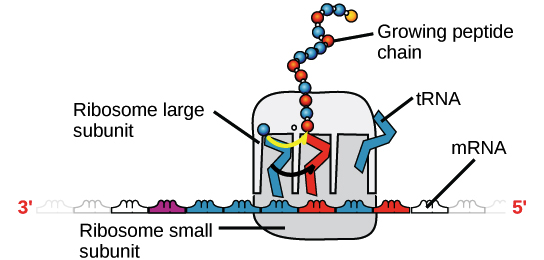
\includegraphics[width=10cm]{mRNAandtRNA}
\end{figure}

\pagebreak
\lr{rRNA}
در ساختار ریبوزوم به کار می‌روند و کمک می‌کنند که
\lr{mRNA}
در جایگاه مناسب قرار بگیرد.
بعضی از
\lr{rRNA}
ها به عنوان آنزیم عمل می‌کنند.
\lr{RNA}
های که به عنوان آنزیم عمل می‌کنند به نام
\lr{ribozymes}
شناخته می‌شوند.

\lr{tRNA}
ساختار سه بعدی دارد که از یک سمت به آمینواسید
\footnote{\lr{amino acid}}
متصل می‌شود. و در سمت دیگر آن سه نوکلئوتید به عنوان کد قرار می‌گیرند تا ریبوزوم با استفاده از آن از روی
\lr{mRNA}
پلی‌پپتید درست را بسازد.

\begin{figure}[htbp]
	\subfloat[ساختار سوم]{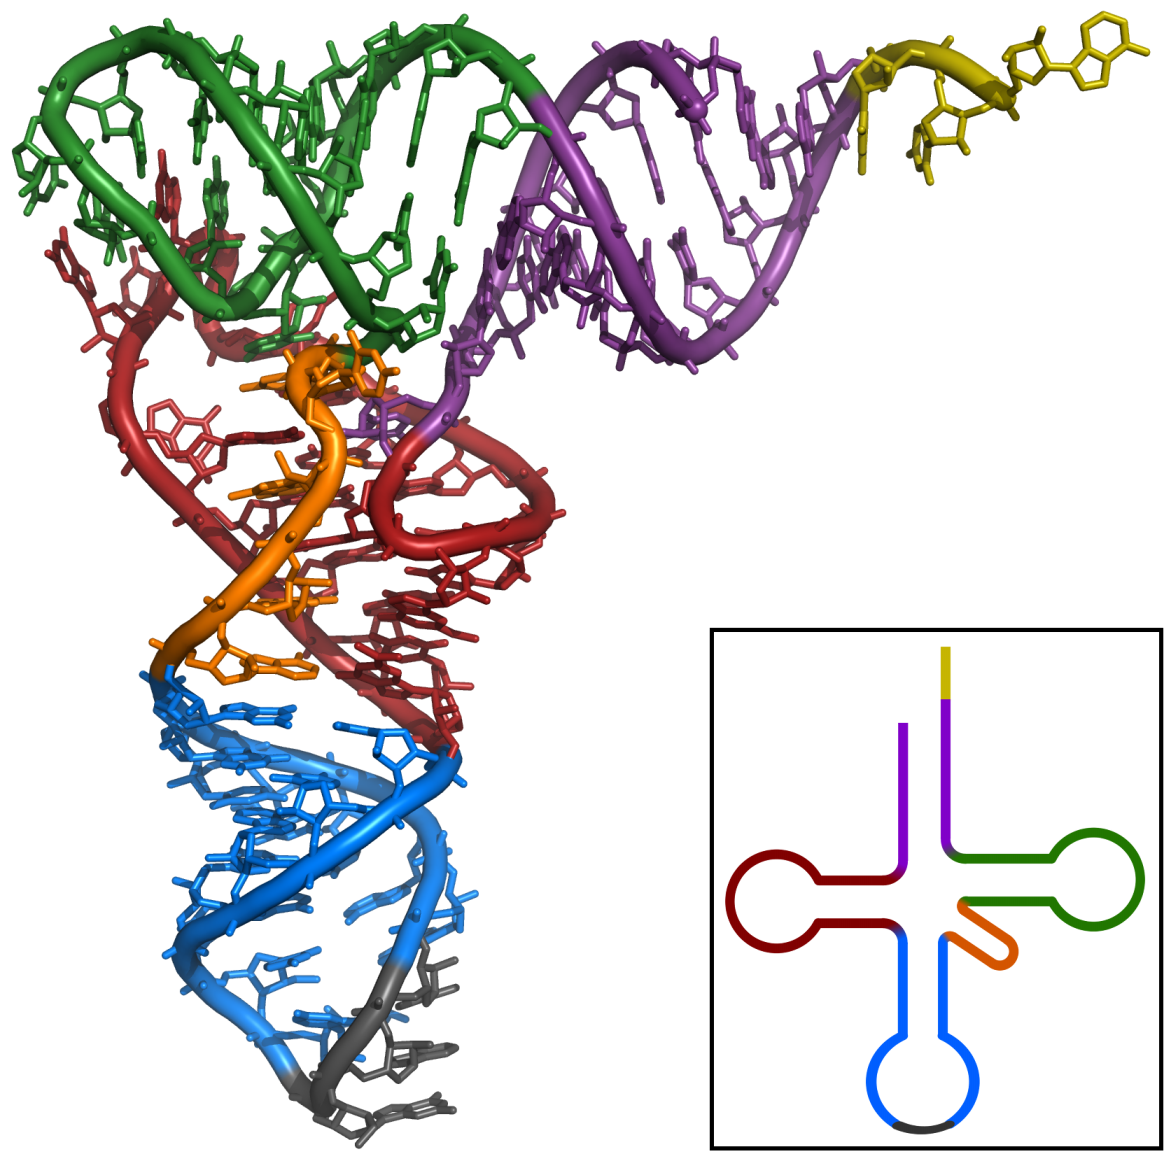
\includegraphics[width=6cm]{trna}}
	\qquad
	\subfloat[ساختار دوم]{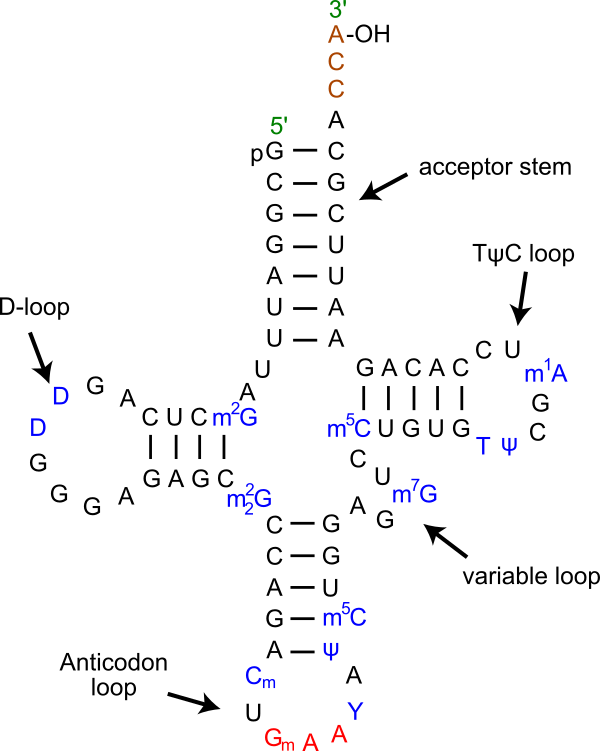
\includegraphics[width=6cm]{trna_second_structure}}
		\caption{مولکول
		\lr{tRNA}}
\end{figure}

یکی از تفاوت‌های مولکول
\lr{RNA}
با مولکول
\lr{DNA}
در این است که در
\lr{RNA}
به جای باز تیمین، باز یوراسیل قرار دارد. گفته می‌شود که یکی از دلایل این جایگزینی این است که باز یوراسیل استحکام کمی دارد و بعد از اینکه
\lr{RNA}
به ساخت
\lr{DNA}
می‌پردازد
آن را با باز تیمین جایگزین می‌کند که استحکام بیشتری دارد.
\cite{MolecularStructureOfRna}

\pagebreak
\subsection{پکیج کردن مولکول دی ان ای در سلول‌های یوکاریوتی\protect\footnote{\lr{DNA packaging}}}

مجموع طول ماده ژنتیکی هر سلول انسانی حدود دو متر است. حال به این می‌پردازیم که چگونه این موجودی دو متری داخل سلول پنج میکرونی جا شده است به طوری که سلول، جایگاه ژن‌های ضروری را می‌داند.

\begin{figure}[htbp]
	\centering
	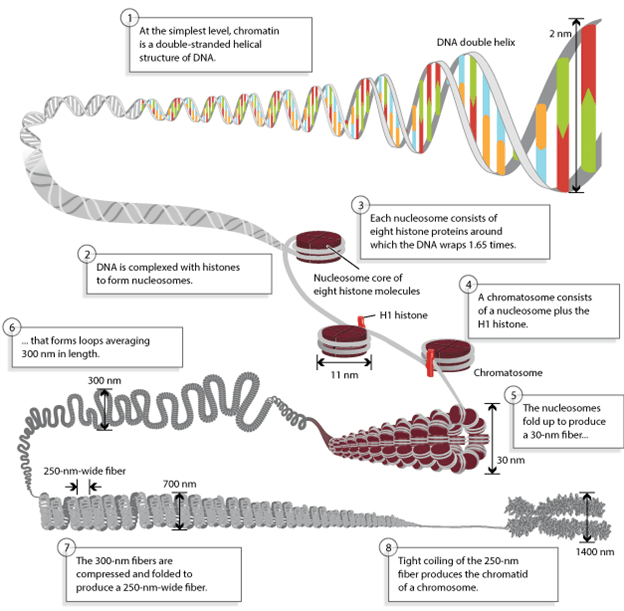
\includegraphics[width = 11cm]{DNA-packaging}
	\caption{پکیج‌کردن مولکول 
	\lr{DNA}}
	\label{figure:dnaPackaging}
\end{figure}

\begin{wrapfigure}[12]{l}{6cm}
	\centering
	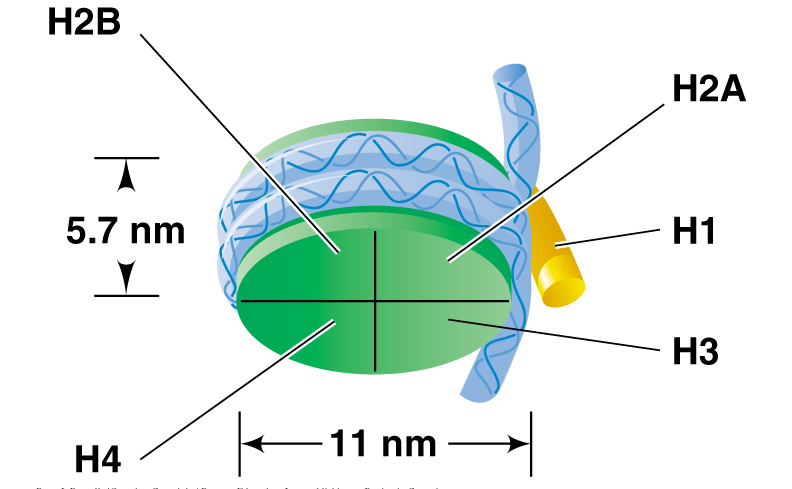
\includegraphics[width=6cm]{Nucleosome}
	\caption{ساختار نوکلئوزوم. از هر کدام از پروتئین‌های نامبرده دو تا کنار هم قرار دارند. 
	\lr{H1}
	جزء نوکلئوزوم نیست.}
	\label{figure:nucleosome}
\end{wrapfigure}


به طور کلی در پکیج کردن مولکول
\lr{DNA}
دو نوع پروتئین به کار میرود:
\begin{itemize}
\item هیستونی
\footnote{\lr{Histones}}
\item غیر هیستونی
\footnote{\lr{Nonhistones}}
\end{itemize}
پروتئین‌های هیستونی بار مثبت دارند و ساختار پایه پکیج کردن یعنی نوکلئوزوم به کمک آن‌ها شکل می‌گیرد.
در مرحله اول هشت مولکول پروتئین در کنار یکدیگر قرار می‌گیرند و سپس رشته
\lr{DNA}
دور آن می‌پیچد به این ساختار یک نوکلئوزوم
\footnote{\lr{Nucleosome}}
گفته می‌شود. نوکلئوزوم به همراه پروتئین
\lr{H1}
کروماتوزوم
\footnote{\lr{Chromatosome}} 
است. تمام پروتئین‌های که در ساختار کروماتوزوم به کار می‌رود هیستونی هستند. همان‌طور که در شکل
\ref{figure:dnaPackaging}
قسمت چهار مشاهده می‌شود به قسمتی از مولکول
\lr{DNA}
که بین دو نوکلئوزوم قرار می‌گیرد
\lr{`Linker'}
گفته می‌شود.
به طور میانگین هر
\lr{Linker}
از 75 جفت باز تشکیل شده است.
در این مرحله قطر ساختار به 11 نانومتر میرسد. 

در مرحله بعد نوکلئوزوم‌ها به کمک پروتئین
\lr{H1}
به هم نزدیک می‌شوند و قطر ساختار را به 30 نانومتر می‌رسانند.

\begin{wrapfigure}[14]{l}{7cm}
	\centering
	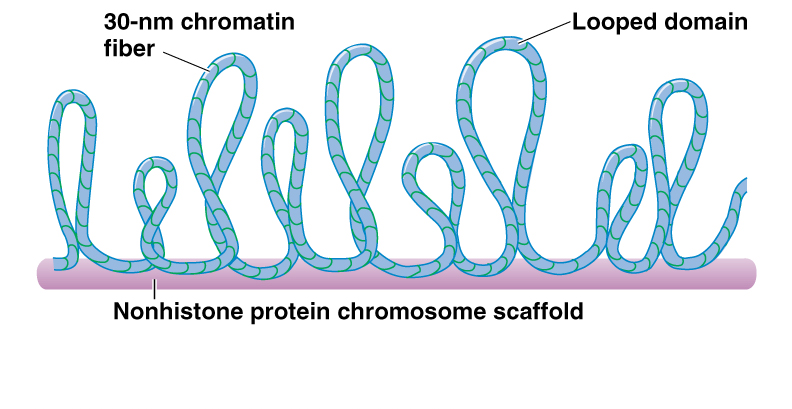
\includegraphics[width=7cm]{DNA-loop}
	\caption{حلقه‌های مولکول 
	\lr{DNA}
	به طول متوسط 300 نانومتر}
	\label{figure:dnaLoop}
\end{wrapfigure}

کروماتینِ 30 نانومتری خم می‌شود و حلقه‌های با طول میانگین 300 نانومتر را می‌سازند. این حلقه‌ها به یک پروتئین غیر هیستونی
(\lr{nonhistone protein scaffolding})
می‌چسبند.

پروتئین‌های غیر هیستونی عموما بار منفی دارند و در نتیجه به سمت پروتئین‌های هیستونی جذب می‌شوند و این در فرآیند پکیج کردن مولکول
\lr{DNA}
مفید است.
پروتئین‌های هیستونی که در مراحل اولیه‌ی پکیج کردن به کار می‌روند دارای تنوع کمی هستند. این تنوع حتی در جانداران متفاوت نیز کم است و طبیعت سعی داشته است با کمترین تغییر‌ آن‌ها را به نسل بعد منتقل کند. اما پروتئین‌های غیر هیستونی که در مراحل انتهایی پکیج کردن به کار می‌روند دارای تنوع بسیار زیادی هستند. هم در جانداران متفاوت فرق دارند و هم در سلول‌های مختلف یک گونه. در واقع همین تفاوت در پروتئین‌های غیر هیستونی است که تفاوت سلول‌ها را بیان می‌کند. همانطور که در شکل
\ref{figure:dnaLoop}
مشخص است نقاطی که در بالای حلقه قرار می‌گیرند احتمال بیشتری برای رونویسی دارند. اینکه کدام قسمت از حلقه در پایین و کدام قسمت در بالا قرار می‌گیرند را پروتئین‌های هیستونی مشخص می‌کنند.

\pagebreak
\subsection{همانندسازی دی ان ای\protect\footnote{\lr{DNA replication}}}

در طی تقسیم سلولی نیاز است که مقدار ماده ژنتیکی دو برابر شود و هر رشته
\lr{DNA}
باید همانند خود را بسازد که به این فرآیند، همانندسازی
\lr{DNA}
گفته می‌شود.

 \begin{wrapfigure}{l}{8cm}
	\centering
	
\includegraphics[width=8cm]{Replication_bubble}
	
\includegraphics[width=8cm]{Space}
	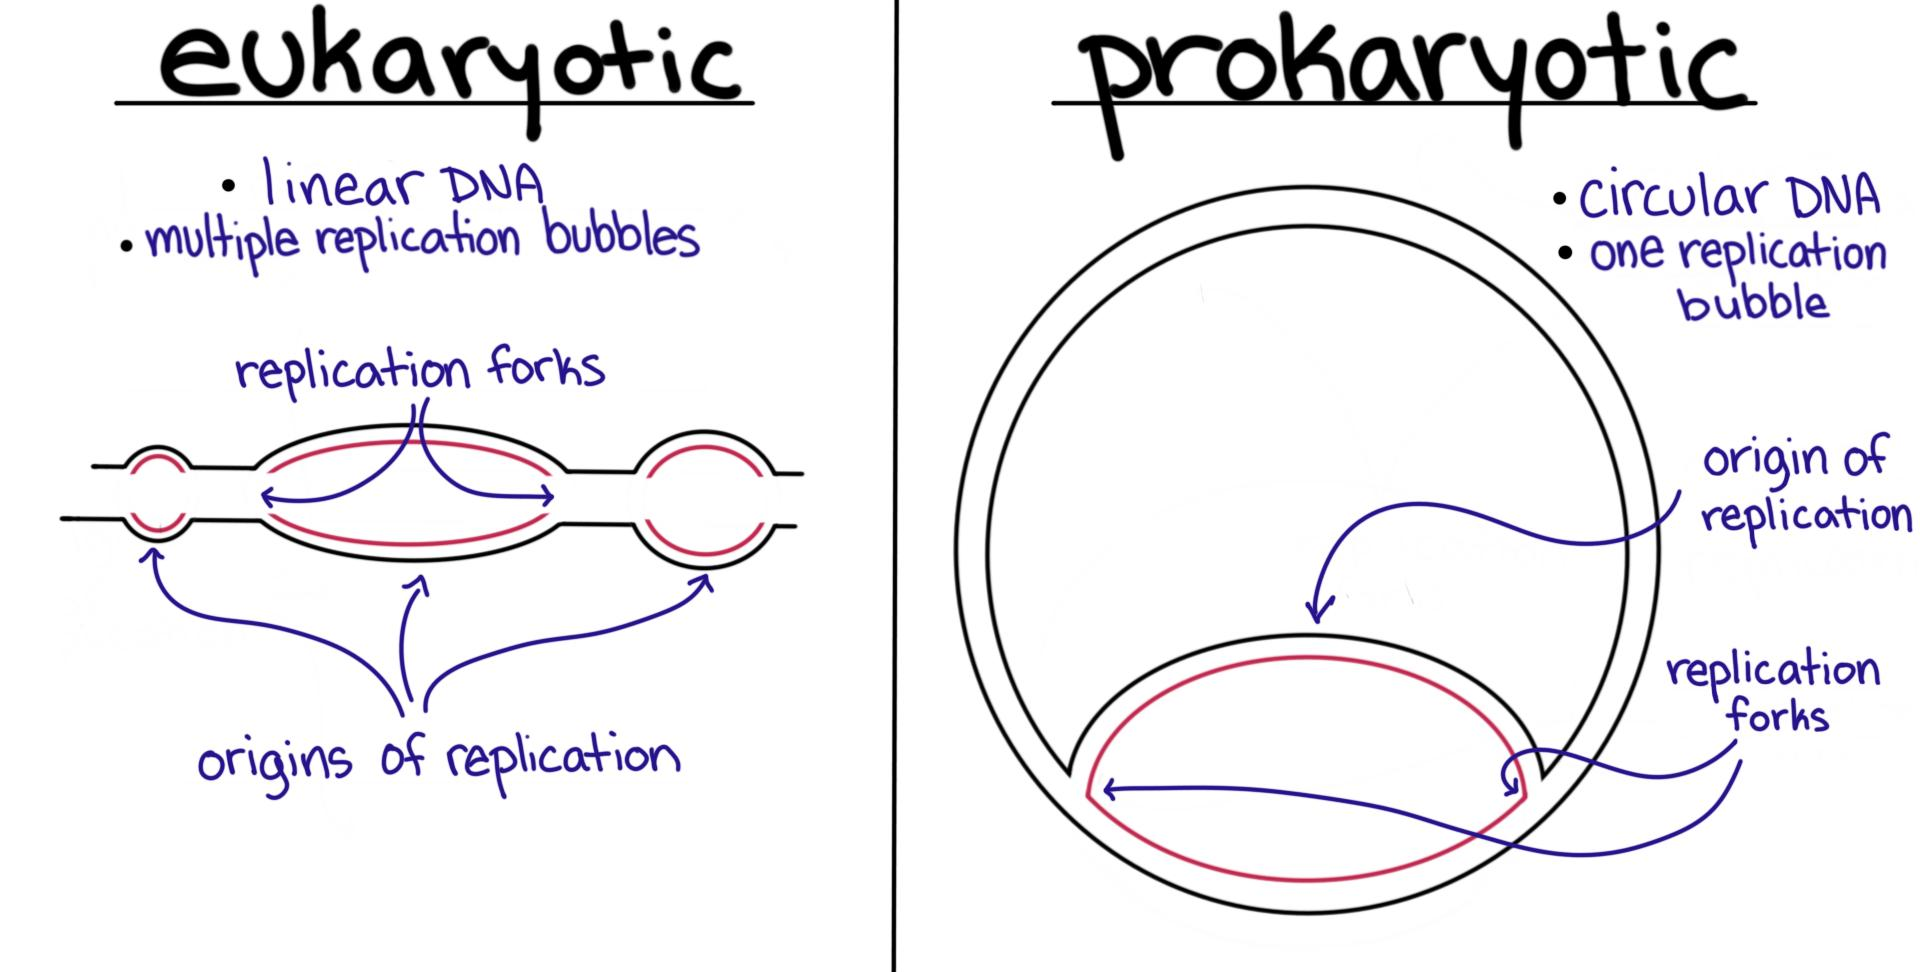
\includegraphics[width=8cm]{cell_eukaryotic_v_prokaryotic_dna_replication}
	\vspace{-20pt}
\end{wrapfigure}

در همانندسازی مولکول
\lr{DNA}
، ابتدا آنزیم هلیکاز
 \footnote{\lr{Helicase}}
 پیوند‌های هیدروژنی را می‌شکند و دو
 \lr{Strand}
 را از هم جدا می‌کند. نقطه‌ای که این گسست شروع می‌شود را 
 \lr{origin point}
 می‌گویند.
 \lr{DNA}
 سلول پروکاریوتی تنها یک
  \lr{origin point}
  دارد اما در سلول یوکاریوتی این نقاط می‌توانند بیشتر باشند و به اصلاح می‌گوید که همانند سازی به صورت موازی
 \footnote{\lr{Parallel}} 
انجام می‌گیرد 
 .
  نقاطی را که هم اکنون در حال باز شدن هستند
  \lr{replication forks}
  می‌نامند.
  
پس از باز شدن رشته توسط آنزیم هلیکاز، آنزیم پرایماز
\footnote{\lr{Primas}}
یک تکه
\lr{RNA}
به یک نخ از رشته
\lr{DNA}
متصل می‌کند که به آن
\lr{RNA primer}
می‌گویند. علت این کار این است که بعد از وصل شد
این قطعه به نخِ رشته
\lr{DNA}
سایر نوکلئوتید‌ها به سمت آن جذب می‌شوند.
  در مرحله بعد به کمک آنزیم
 \lr{DNA}
 پلیمراز
 \RN{3}
 \footnote{\lr{DNA polymerase \RN{3}}}
 نوکلئوتید‌های مکمل که درون غشا قرار دارند در مقابل نخ
 قرار می‌گیرند.
 
 برای فهم کامل همانندسازی باید به ساختار مولکول
 \lr{DNA}
 توجه کنیم. همانطور که قبلا گفته شد دو رشته مولکول
 \lr{DNA}
 به صورت
 \lr{antiparallel}
 در مقابل همدیگر قرار می‌گیرند به این معنی که یکی در جهت
$ 5^\prime $
  به
$ 3^\prime $
  است و دیگری در جهت
$ 3^\prime $
  به
$ 5^\prime $
.
و اما نکته‌ای که وجود دارد این است که آنزیم
\lr{DNA}
پلیمراز
تنها در جهت
$ 3^\prime $
  به
$ 5^\prime $
می‌تواند حرکت کند چرا که ساخت پروتئین تنها در جهت
$ 5^\prime $
  به
$ 3^\prime $
انجام می‌شود
.
شکل
\ref{figure:dnaReplication}
را مشاهده کنید.
در نتیجه این آنزیم ابتدا روی یکی از رشته‌ها که به آن
\lr{leading strand}
گفته می‌شود، حرکت می‌کند. برای رشته مقابل یعنی
\lr{lagging strand}
از سمت
\lr{replication fork}
به سمت
\lr{origin point}
حرکت می‌کند.
همانندسازی
\lr{leading strand}
به صورت پیوسته است اما در
\lr{lagging strand}
،
\lr{DNA}
پلیمراز
مجبور است همانندسازی را در قطعه‌هایی به اسم
\lr{Okazaki fragment}
انجام دهد. توجه کنید که در
\lr{lagging strand}
به ازای هر
\lr{Okazaki fragment}
ابتدا آنزیم
\lr{Primase}
یک
\lr{RNA Primer}
بر روی نخِ رشته قرار می‌دهد.  اما در
\lr{leading strand}
تنها یک
\lr{RNA Primer}
کافی است.


\begin{figure}[htbp]
	\centering
	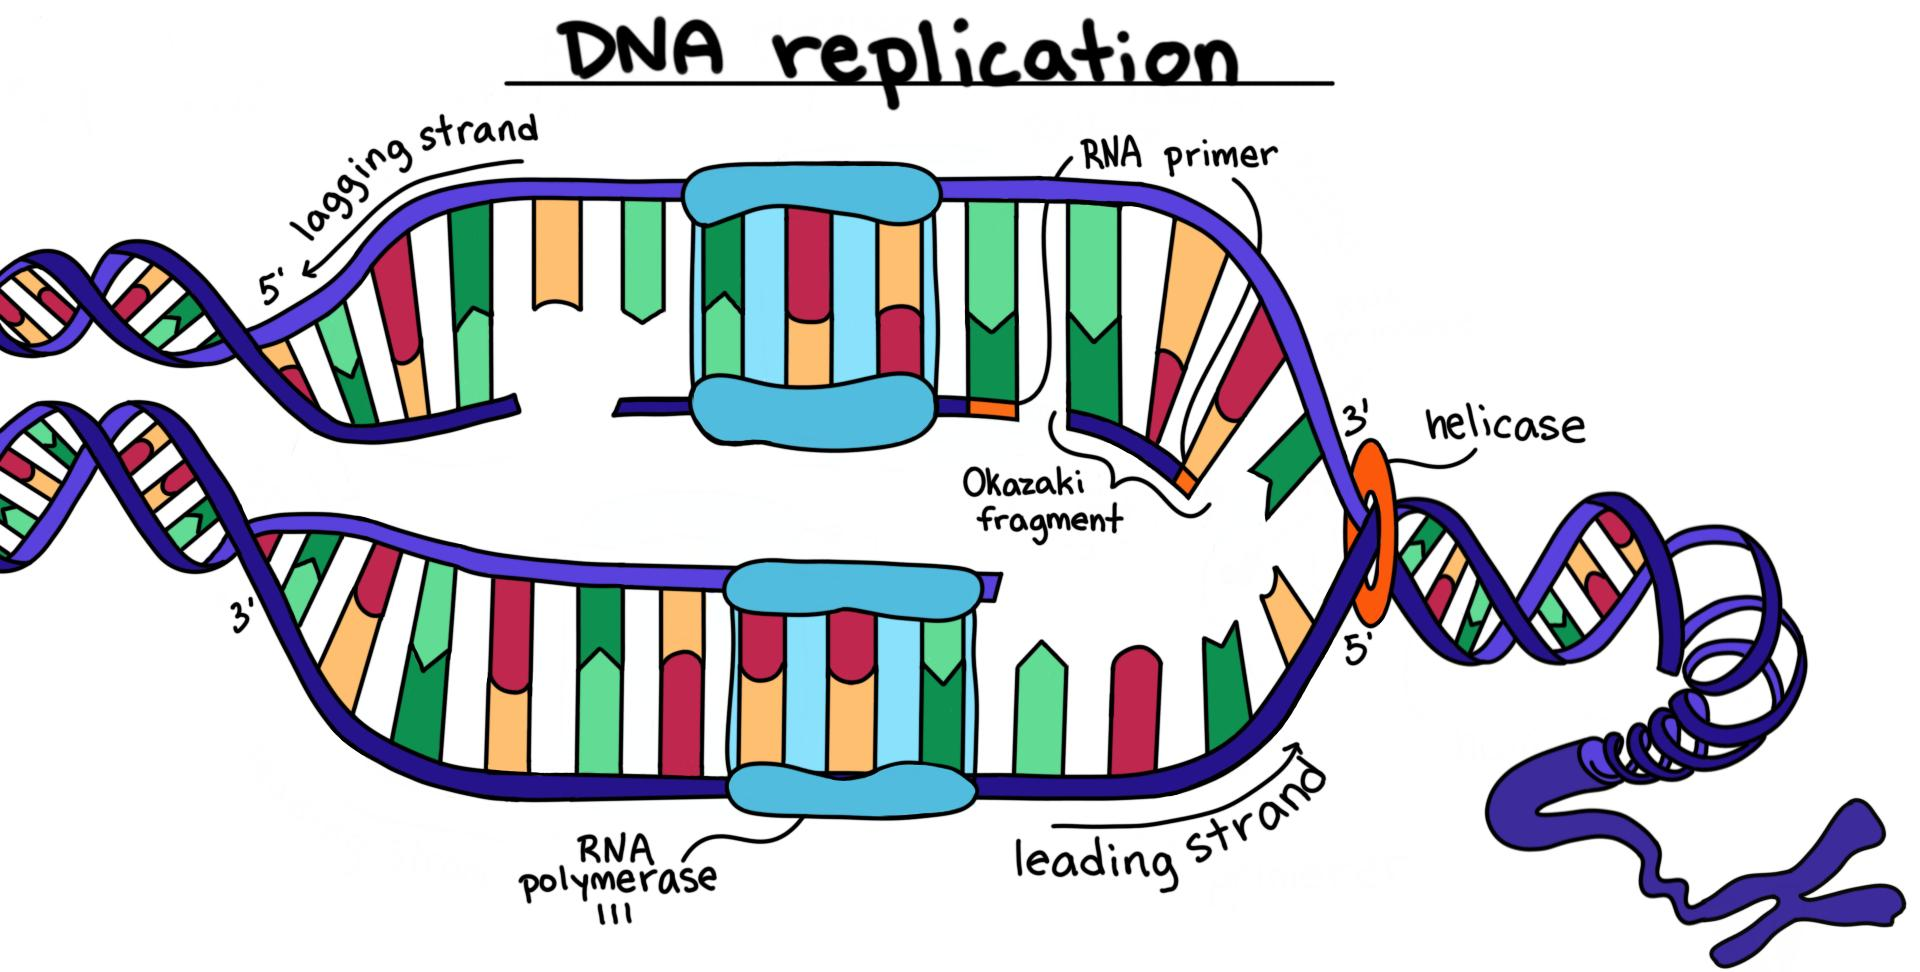
\includegraphics[width=10cm]{dna_replication_eukaryotic}
	\caption{همانندسازی 
	\lr{DNA}
	به کمک دو آنزیم هلیکاز و  
	\lr{DNA} 
	پلیمراز
	در سلول یوکاریوتی
	}
	\label{figure:dnaReplication}
\end{figure}

\pagebreak
\begin{wrapfigure}{l}{8cm}
	\centering
	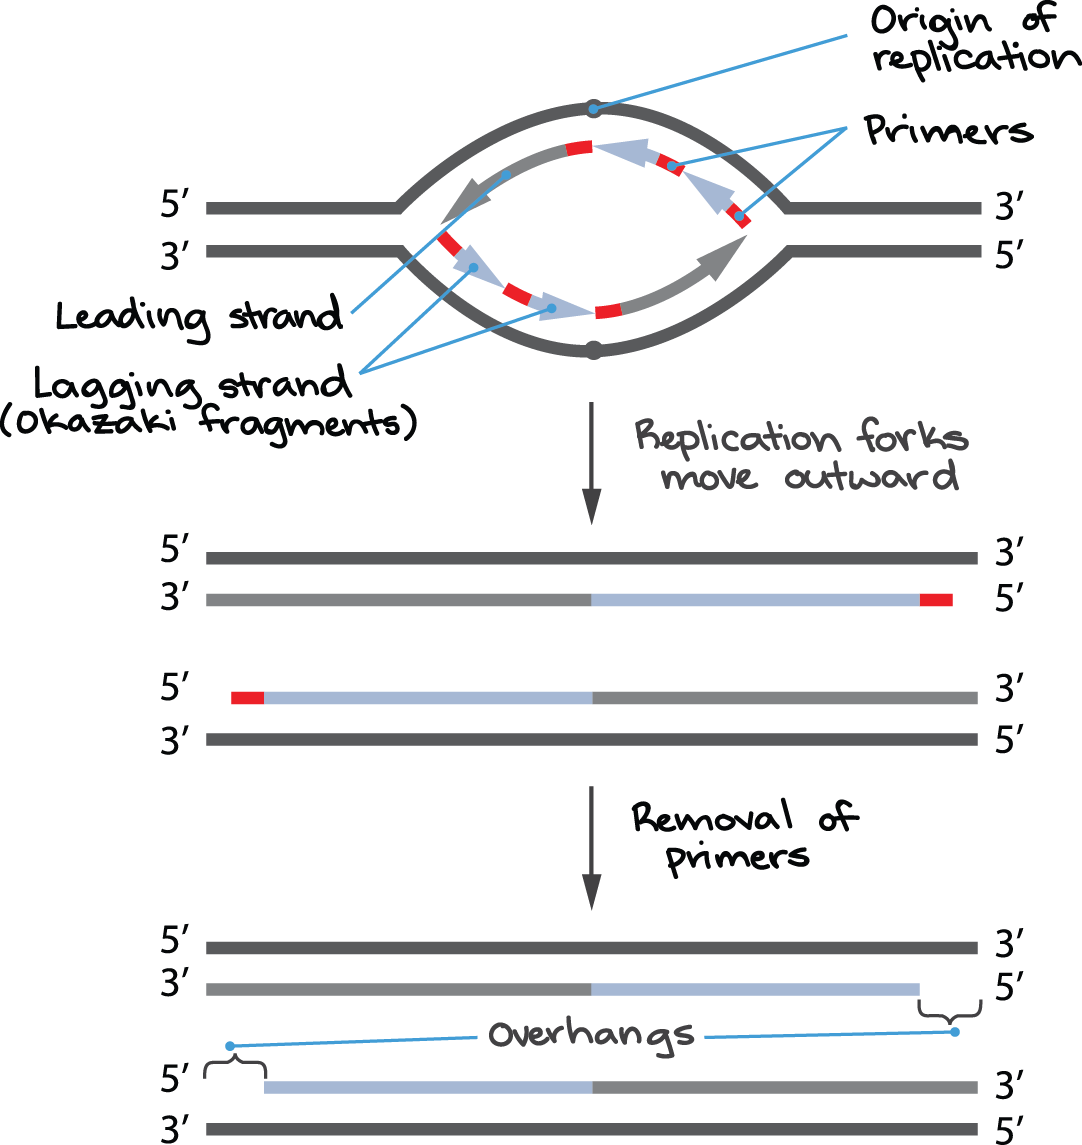
\includegraphics[width=8cm]{Worn_off_of_telomeres}
\end{wrapfigure}

\begin{figure}[htbp]
	\centering
	\subfloat[]{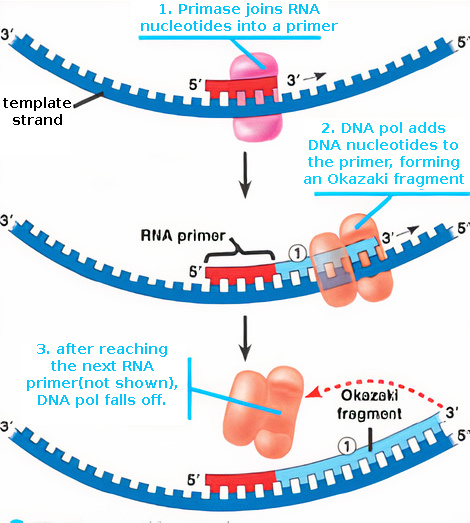
\includegraphics[width=6.5cm]{Replication_one}}
	\hspace{20pt}	
	\subfloat[]{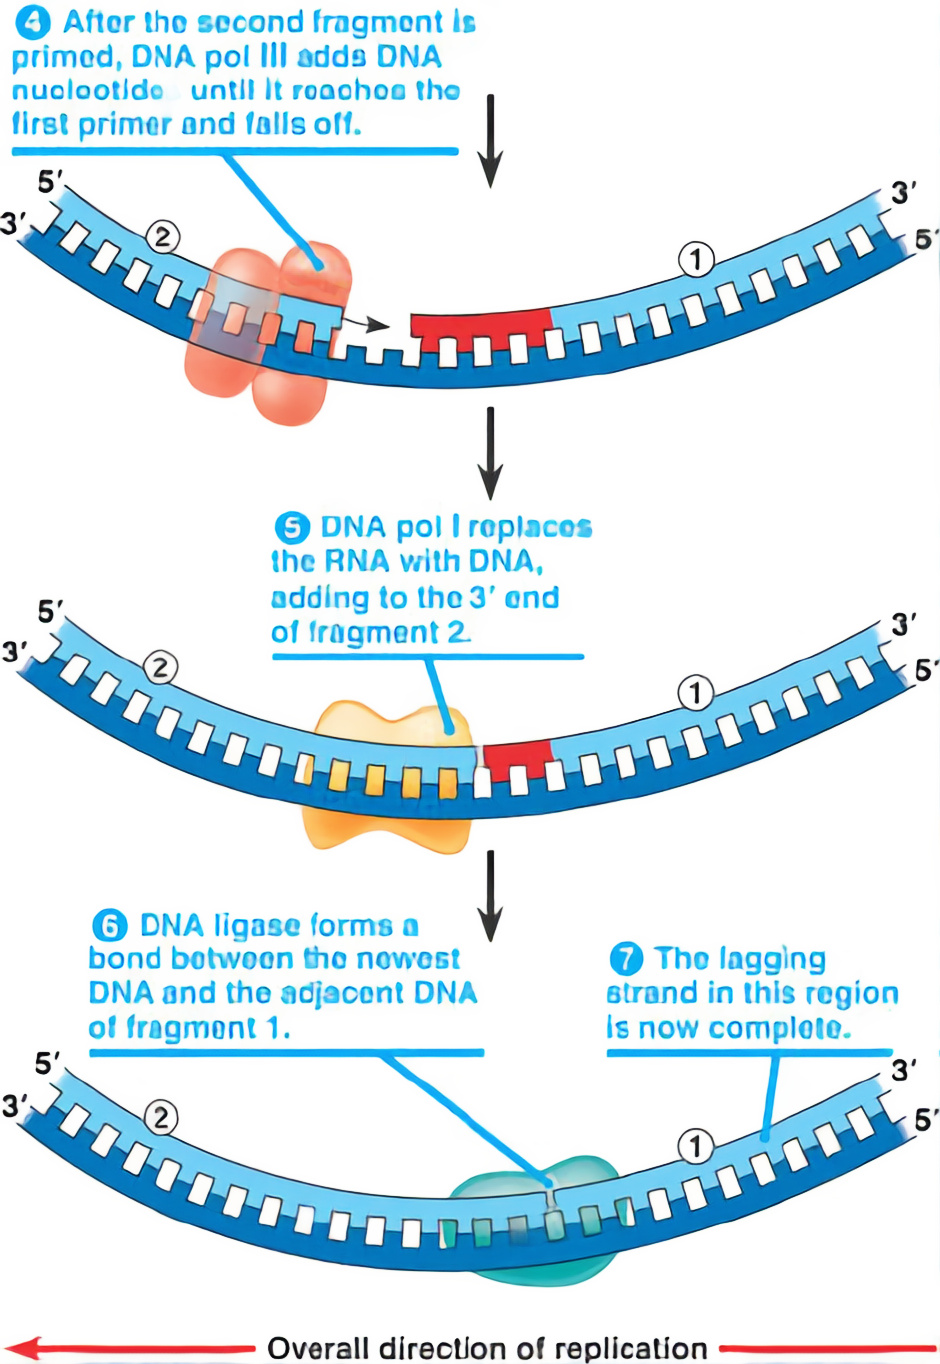
\includegraphics[width=6.5cm]{Replication_two}}
	\caption{مراحل همانندسازی دی ان ای}
	\label{figure:replication_sections}
\end{figure}

بعد از انجام همانند سازی توسط
 \lr{DNA}
 پلیمراز
 \RN{3}
 نیاز است که
 \lr{RNA Primer}
 ها حذف شوند و جای آن‌ها نخِ
 \lr{DNA}
 قرار گیرد.  در
\lr{lagging strand}
 بعد از تمام شدن هر
\lr{Okazaki fragment}
،
\lr{DNA}
پلیمراز
\RN{1}
،
\lr{RNA primer}
ای که مربوط به
\lr{Okazaki fragment}
قبلی است را با
\lr{DNA}
جایگزین می‌کند. سپس آنزیم
\lr{DNA}
لیگاز
\footnote{\lr{DNA ligase}}
پیوند بین دو تکه رشته
\lr{DNA}
را برقرار می‌کند.
به شکل
\ref{figure:replication_sections}
توجه کنید.
در سلول‌های پروکاریوتی نیز با توجه به اینکه کروموزوم حلقوی دارند، بعد از اتمام همانندسازی در یک جهت
\lr{DNA}
پلیمراز
\RN{3}
به
\lr{RNA primer}
می‌رسد و در نتیجه
\lr{DNA}
پلیمراز
\RN{3}
رشته را رها می‌کند و
\lr{DNA}
پلیمراز
\RN{1}
،
\lr{RNA primer}
را با
\lr{DNA}
جایگزین می‌کند.
در سلول‌های یوکاریوتی جایگاه اولین پرایماز در انتهای کروموزوم توسط
\lr{DNA}
پلیمراز
\RN{3}
تشخیص داده نمی‌شود در نتیجه این قسمت از
\lr{DNA}
از بین می‌رود و در نتیجه در هربار انجام همانندسازی مقدار کمی از دم کروموزوم از بین می‌رود.
برای جلوگیری از بین رفتن ژن‌ها کروموزوم یوکاریوتی قسمتی به اسم
تلومر
\footnote{\lr{telomeres}}
دارد. در واقع تلومر در دو سر کروموزوم قرار دارد. تلومر از تکرار صدها یا هزاران بارِ یک دنباله کوتاه
\lr{DNA}
تشکیل شده است. این دنباله در جانداران مختلف فرق دارد اما در انسان و سایر پستانداران به صورت
$ 5^\prime-TTAGGG-3^\prime $
است.
تلومر عمر انسان را مشخص می‌کند چرا که با کوتاه شدن تلومر ژن‌های حساس نیز از بین می‌روند و عملکرد سلول مختل می‌شود. در واقع به همین خاطر است که سلول تعداد محدودی تقسیم انجام می‌دهد.

\begin{wrapfigure}[14]{l}{9cm}
	\centering
	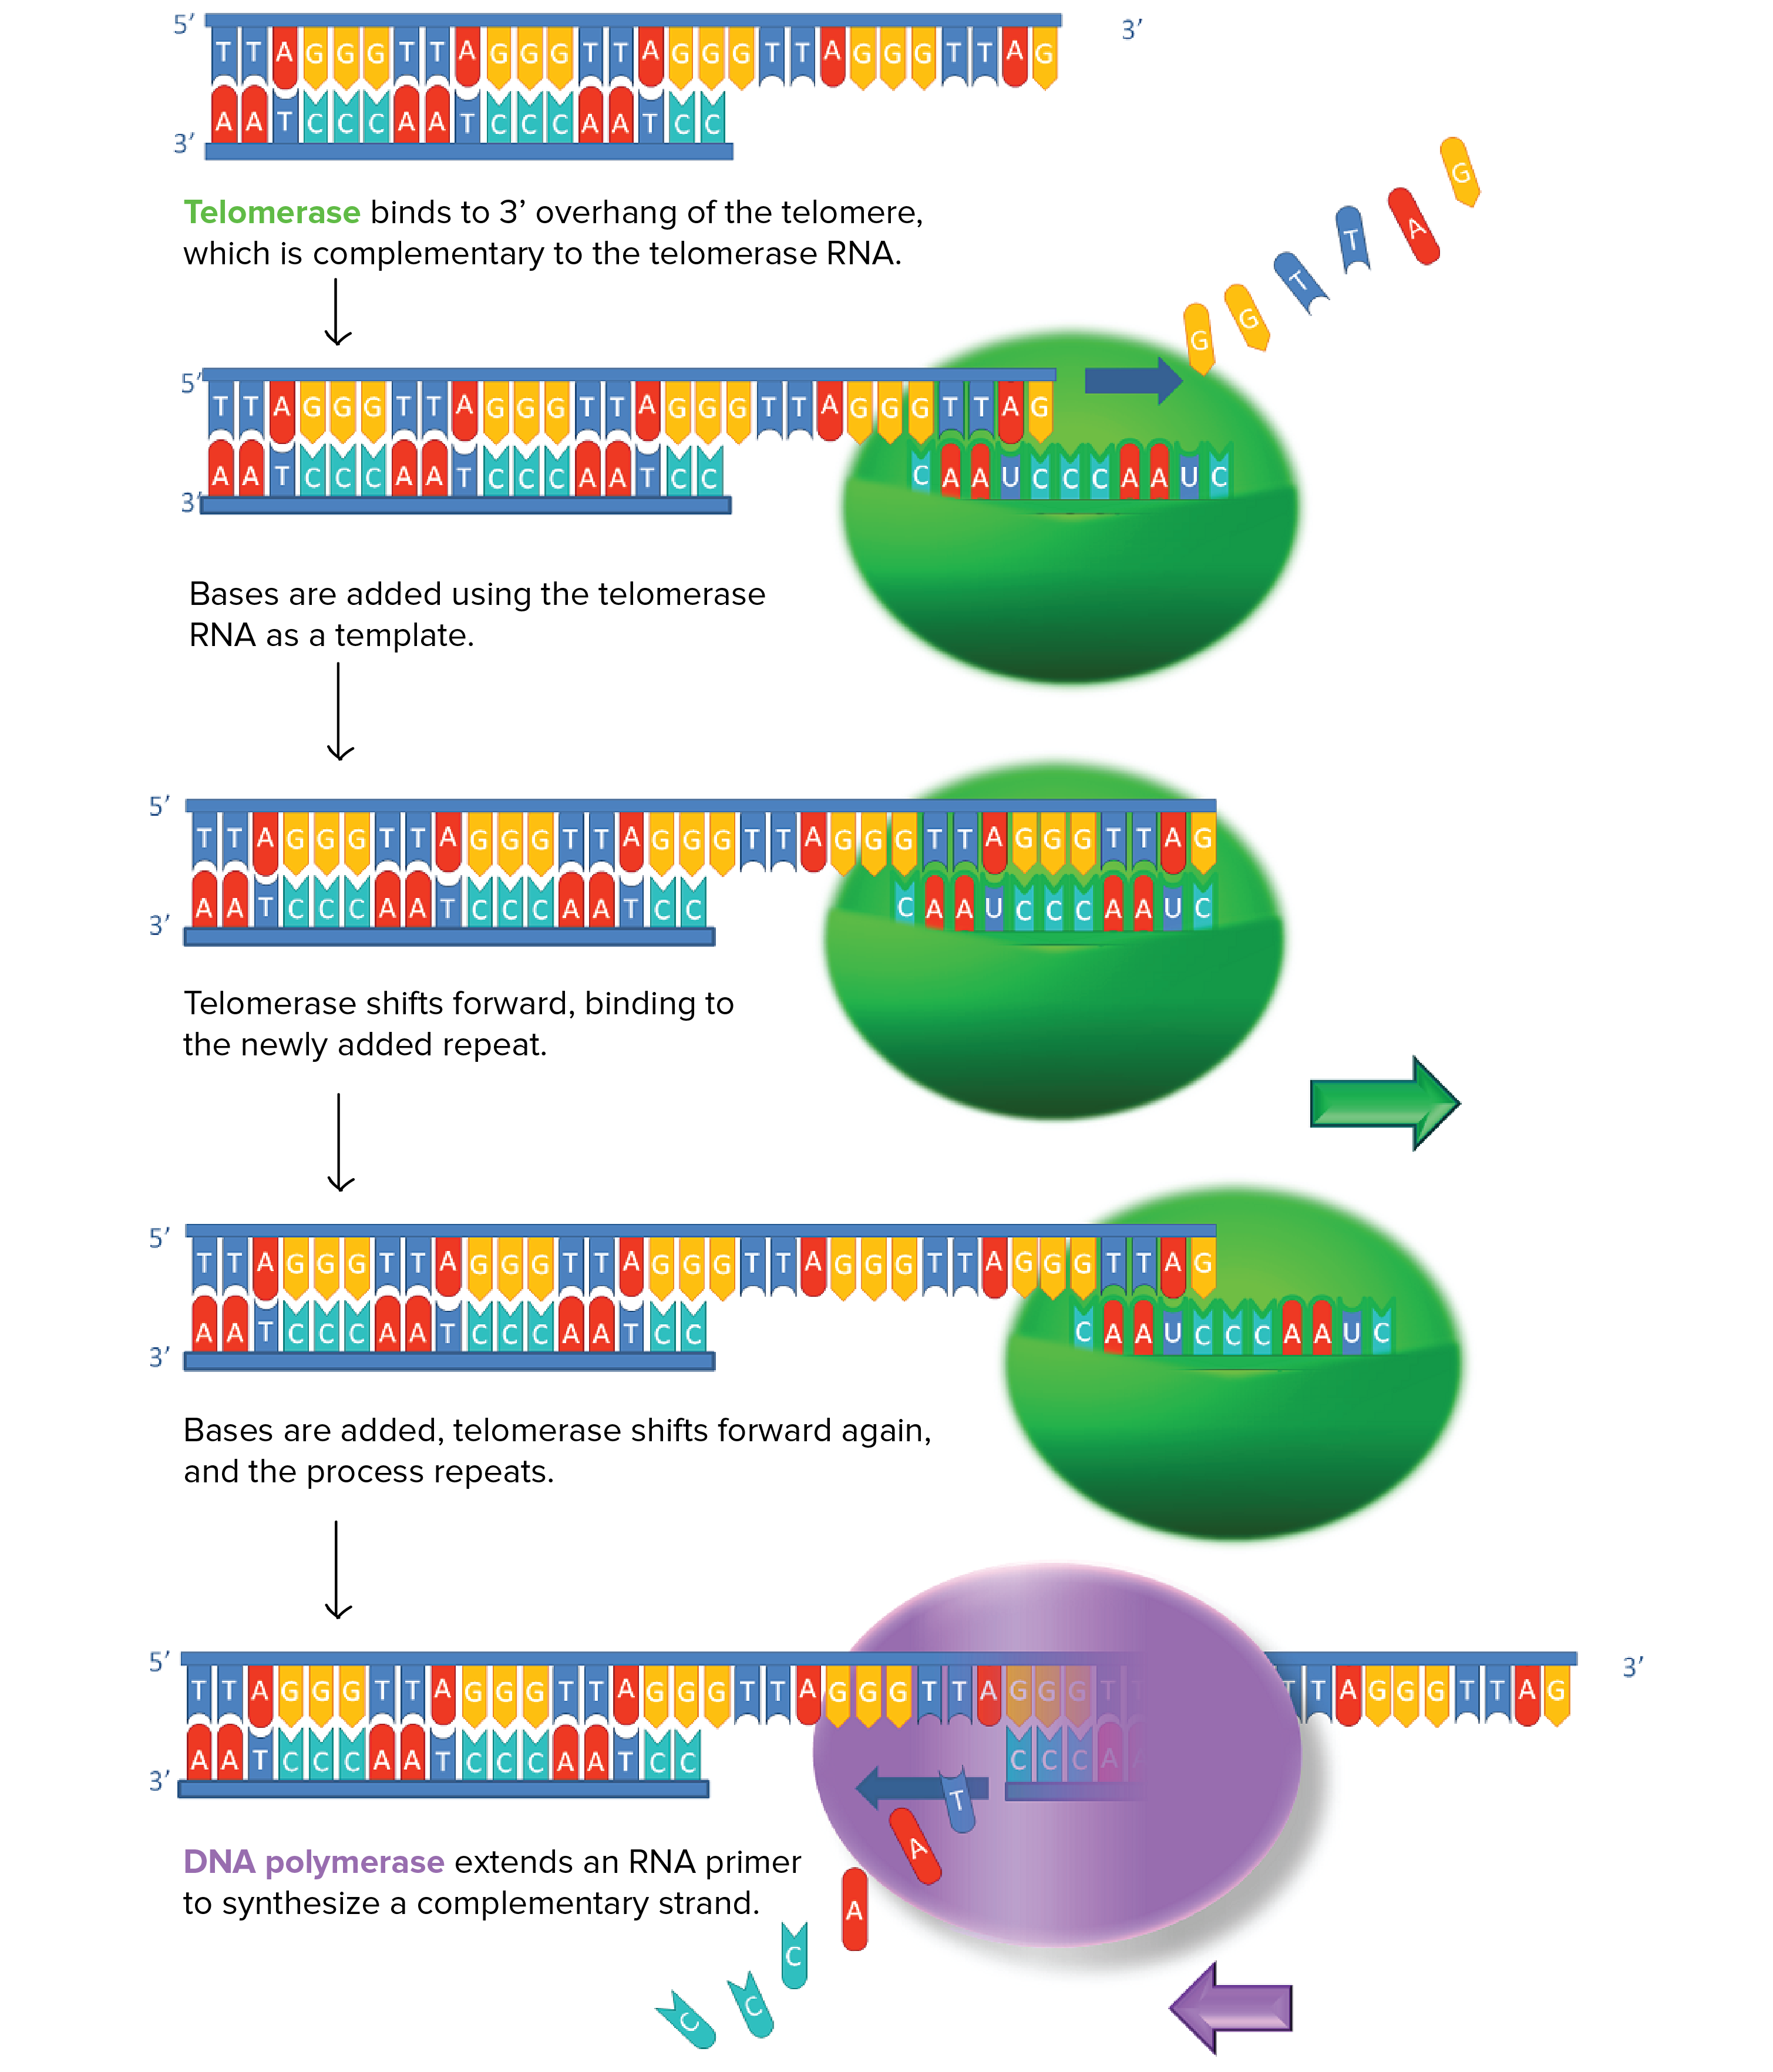
\includegraphics[width=9cm]{Telomerase_function}
	\caption{ انزیم تلومراز از کوتاه شدن 
	\lr{DNA}
	در سلول‌های جنسی جلوگیری می‌کند.}
	\label{figure:TelomeraseFunction}
\end{wrapfigure}

نکته‌ای که وجود دارد این است که اگر این کوتاه شدن تلومر در سلول‌های جنسی نیز اتفاق بیافتد، نسل به نسل ماده ژنتیک کوتاه می‌شود و در نتیجه گونه منقرض می‌شود. به همین علت آنزیمی به اسم تلومراز
\footnote{\lr{Telomerase}}
یک تکه اضافه به انتهای کروموزوم اضافه می‌کند.
در شکل
\ref{figure:TelomeraseFunction}
نحوه عملکرد این آنزیم نشان داده شده است.

در رشته جدید ایجاد شده یک
\lr{Strand}
از رشته قبلی گرفته شده و یک
\lr{Strand}
توسط آنزیم 
\lr{DNA}
پلیمراز ساخته شده است به همین علت گفته می‌شود که همانندسازی
\lr{DNA}
به صورت نیمه حفظ شده
\footnote{\lr{Semi conservative}}
 است.

آنزیم
\lr{DNA}
پلیمراز عمل دیگری نیز انجام می‌دهد که ویرایش
\footnote{\lr{proofriding}}
نام دارد. طی ویرایش آنزیم روی رشته حرکت می‌کند و اگر نوکلئوتیدی به اشتباه در رشته قرار گرفته باشد با نوکلئوتید درست جایگزین می‌کند.

\pagebreak
\subsection{آغاز همانندسازی دی ان ای در ای کولای\protect\footnote{\lr{E. coli}}}

همانندسازی دی ان ای در ای کولای سه مرحله دارد:
\begin{itemize}
\item \lr{chain initiation}
\item \lr{chain extension}
\item \lr{chain termination}
\end{itemize}

باکتری
\lr{E. coli}
دارای یک کروموزوم حلقوی است. این کروموزوم حلقوی دارای دنباله‌ای کوتاه از نوکلئوتید‌ها است که
\lr{replication origin (oriC)}
نام دارد.
\lr{oriC}
مخفف
\lr{\textcolor{red}{Ori}gin of \textcolor{red}{C}hromosomal}
است.
\lr{oriC}
دارای 245 جفت‌باز است که نسبت به سایر باکتری‌ها به شدت محافظت می‌شود.

\lr{oriC}
دارای چند نوع ناحیه مهم است که در شروع همانند‌سازی اهمیت دارند:

\begin{description}
\item[\lr{R sites}]
\lr{oriC}
دارای 5 جایگاه
\lr{R}
است که هر کدام از 9 جفت نوکلئوتید تشکیل شده‌اند.  این 5 جایگاه یک
\lr{binding site}
برای پروتئین آغاز کننده یعنی
\lr{DnaA}
ایجاد می‌کنند.
\item[\lr{I sites}]
این جایگاه‌ها نیز میزبان
\lr{DnaA}
هستند.
\item[\lr{DNA unwinding element (DUE)}]
دنباله‌ای از سه بار تکرار 13 جفت‌باز است که جفت‌باز‌های
\lr{A--T}
در آن زیاد است. با توجه به اینکه بین باز آدنین و تیمین دو پیوند هیدروژنی برقرار می‌شود وقتی ناحیه غنی از این جفت‌باز باشد نسبتا سست‌تر است و آسان‌تر گسسته می‌شود.
\item[\lr{binding site for the protein IHF}]
(
\lr{IHF}
مخفف
عامل میزبان ادغام
\footnote{\lr{integration host factor}}
است.
)
\item[\lr{binding site for the protein FIS}]
(
\lr{FIS}
مخفف
عامل تحریک وارونگی
\footnote{\lr{factor for inversion stimulation}}
است.
)
\item[\lr{GATC methylation sites}]
جایگاه‌هایی برای گروه متیل
\end{description}

\begin{figure}[htbp]
	\centering
	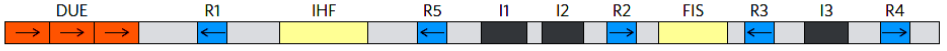
\includegraphics[width=10cm]{Ecoli_elememts_of_oric}
\end{figure}

\begin{figure}[htbp]
	\centering
	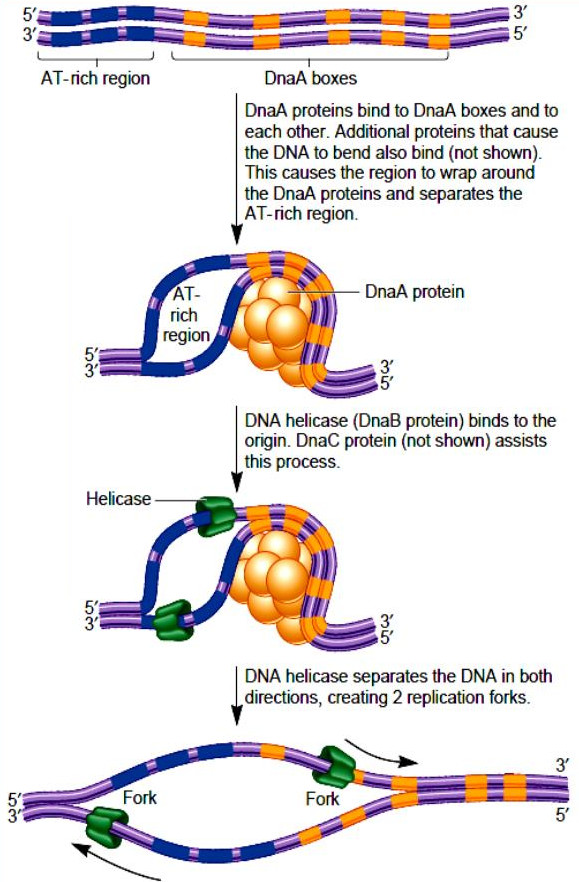
\includegraphics[width=7cm]{Ecoli_replication_origin}
	\caption{آغاز همانندسازی در ای کولای}
	\label{figure:ecoliInitialReproduction}
\end{figure}

\begin{wrapfigure}{l}{6cm}
	\centering
	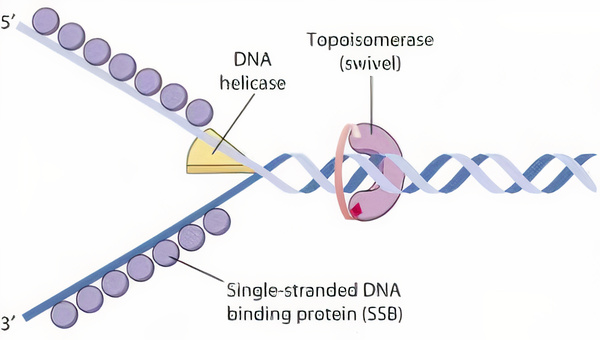
\includegraphics[width=6cm]{Single_stranded_binding_proteins}
	\caption{\lr{Single stranded binding proteins and topoisomerase}}
	\label{figure:SingleStrandedBindingProteins}
\end{wrapfigure}

همانطور که در شکل
\ref{figure:ecoliInitialReproduction}
مشخص است پروتئین
\lr{DnaA}
به همراه چند پروتئین دیگر
به
\lr{DnaA box}
ها میچسبد و این باعث می‌شود تا
\lr{AT-rich region}
باز شود سپس دو آنزیم هلیکاز به دو سمت این
\lr{Replication bubble}
می‌چسبند و شروع به باز کردن بیشتر این ناحیه می‌کنند.

همانطور که در شکل
\ref{figure:SingleStrandedBindingProteins}
مشاهده می‌کنید با حرکت هلیکاز به سمت جلو دو اتفاق می‌افتد اول اینکه ممکن است رشته پشت سر آن دوباره به هم بچسبد به همین خاطر پروتئین‌هایی به نام
\lr{Single Stranded Binding Protein}
به دو نخِ رشته
\lr{DNA}
پیچسبند تا فرصت برای همانندسازی این قسمت فراهم شود. دوم اینکه با حرکت هلیکاز به سمت جلو رشته
\lr{DNA}
در جلو آن فشرده می‌شود به همین خاطر
\lr{Topoisomerase}
رشته
\lr{DNA}
را می‌چرخاند تا فشردگی آن کم شود یا به اصطلاح از
\lr{over winding}
جلوگیری می‌کند.

\begin{figure}[htbp]
	\centering
	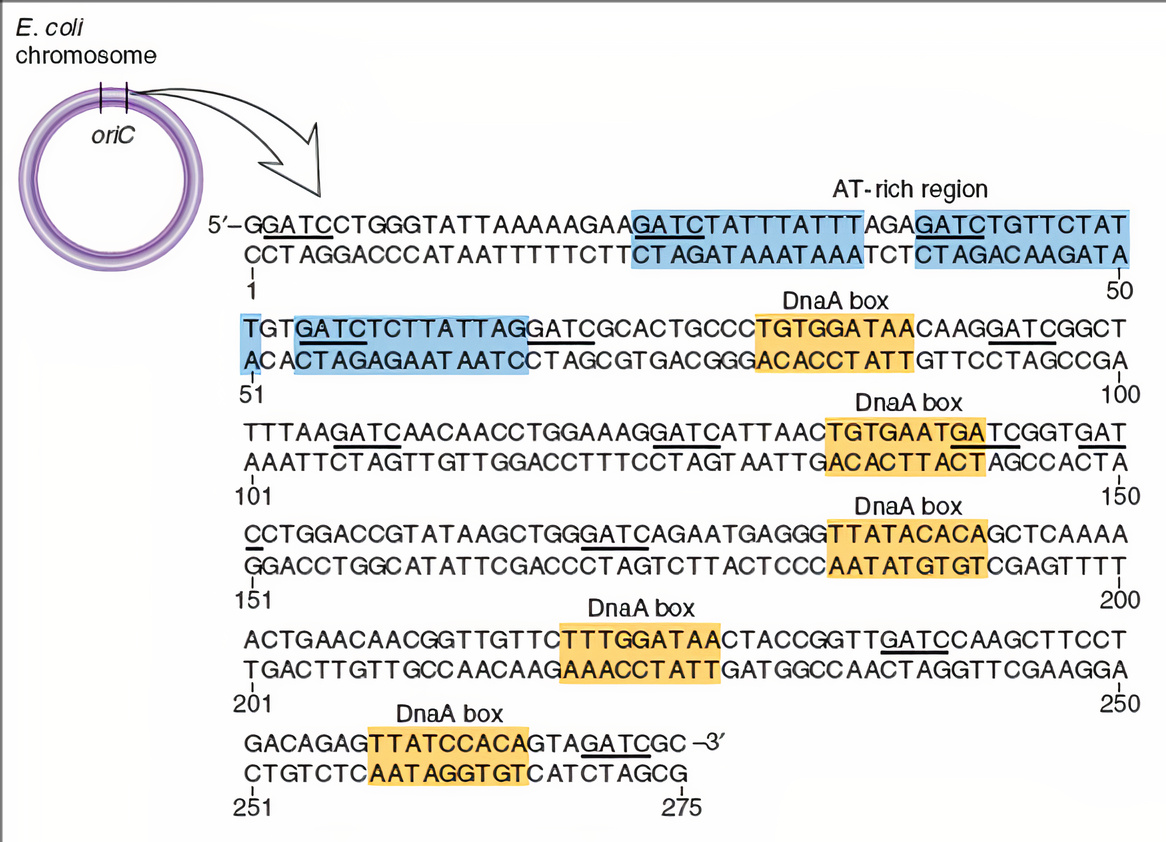
\includegraphics[width=8cm]{ecoli_oric_sequence}
\end{figure}

\pagebreak
\subsection{تقسیم سلولی}
\subsubsection{تقسیم دوتایی در باکتری‌ها\protect\footnote{\lr{Binary fission}}}

\begin{wrapfigure}[15]{l}{10cm}
	\centering
	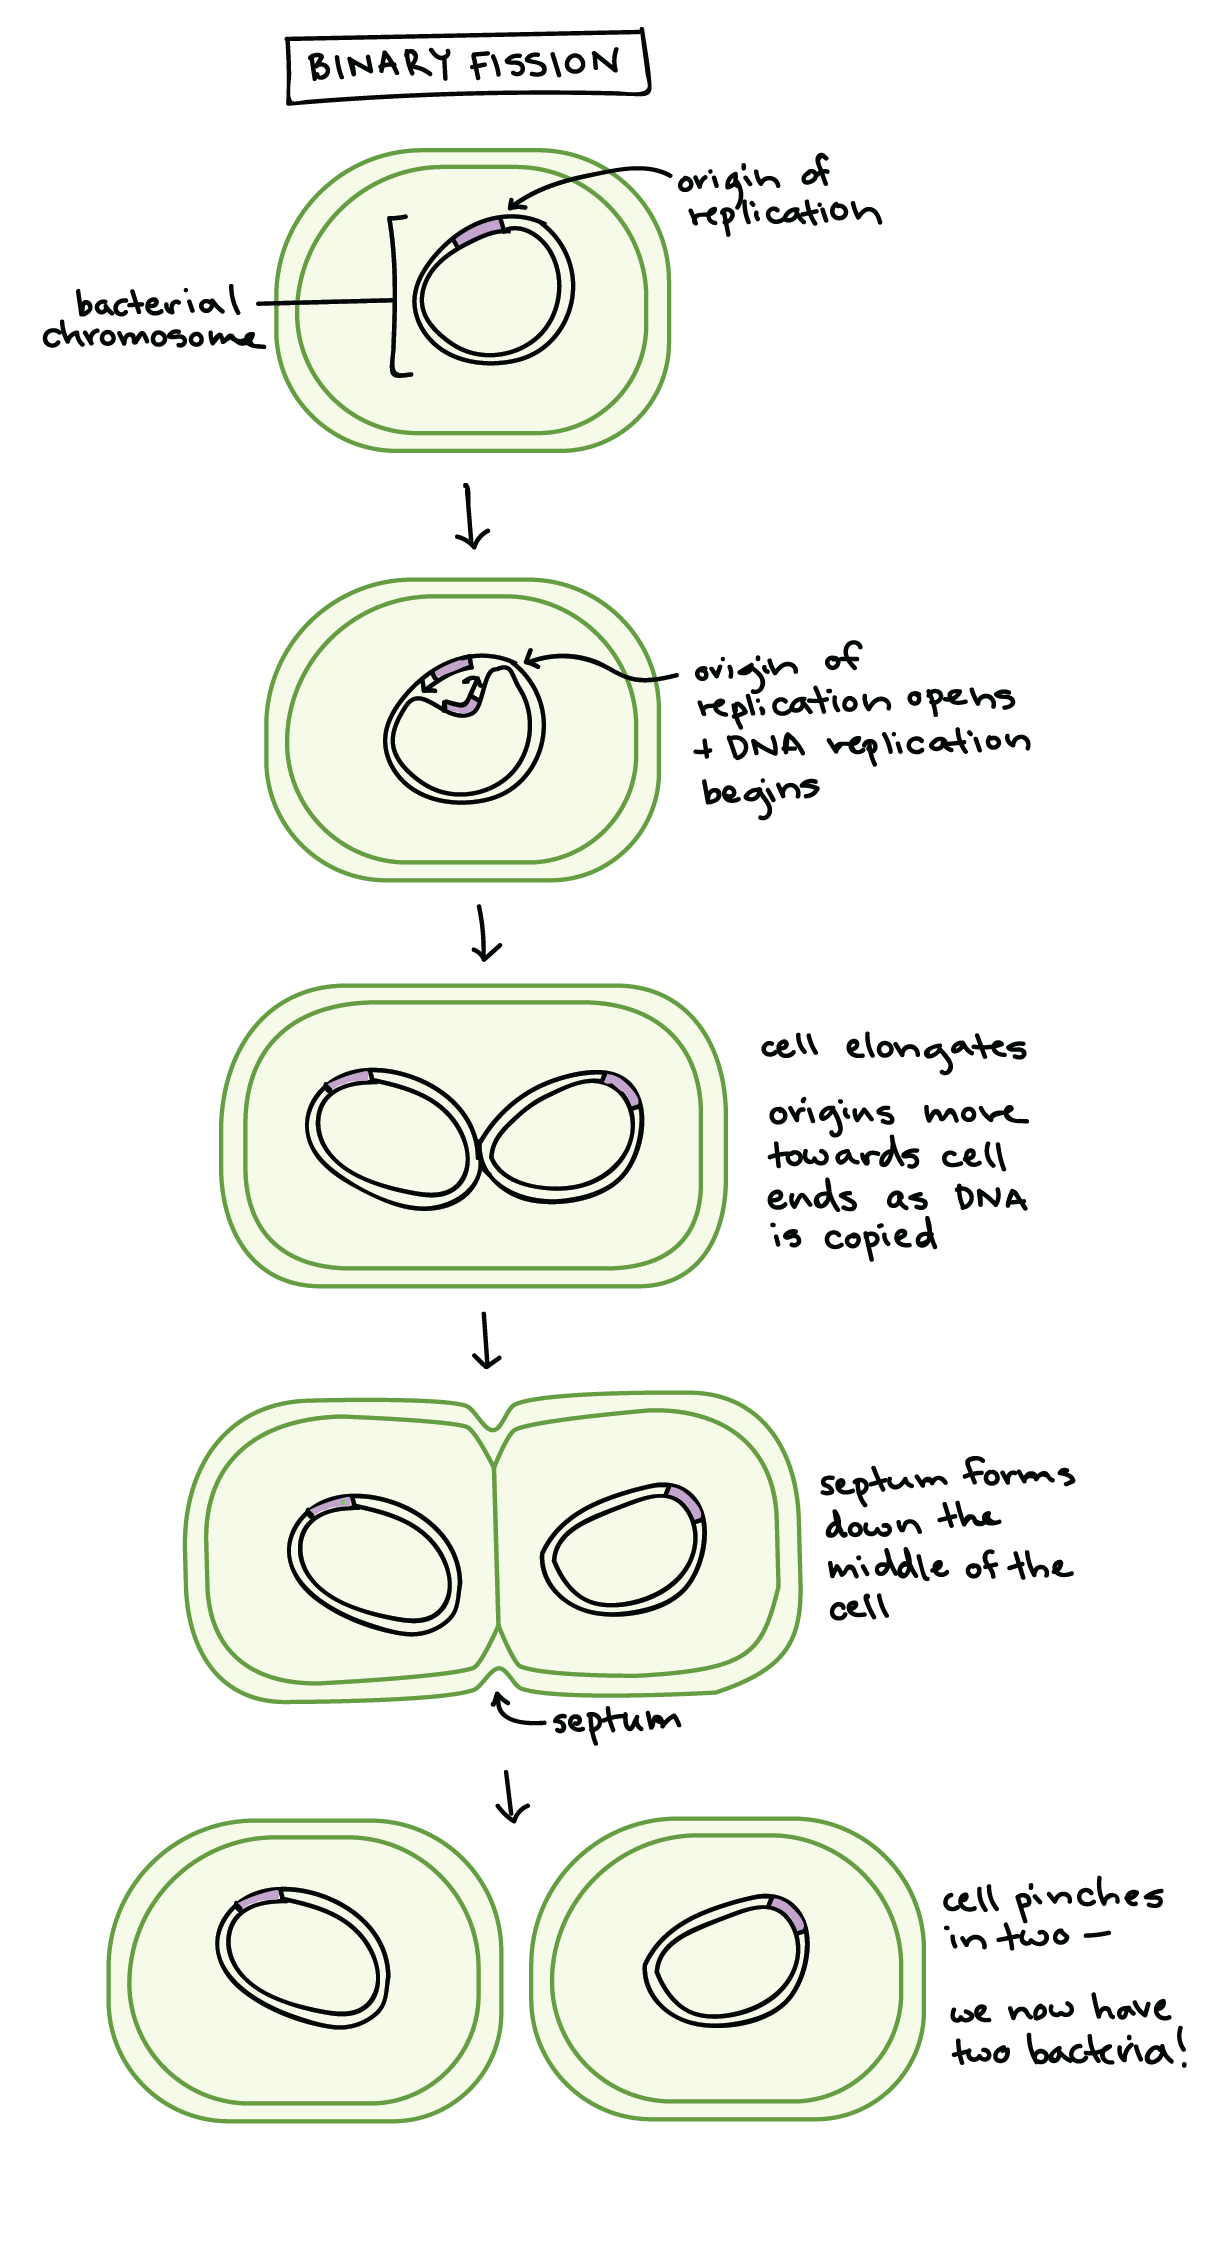
\includegraphics[width=10cm]{Binary_fission}
\end{wrapfigure}

تقسیم سلولی در جاندارانی مثل باکتری‌ها ساده‌تر از تقسیم سلولی در یوکاریوت‌ها است. باکتری‌ها دارای
\lr{DNA}
حلقوی هستند و به روش تقسیم دوتایی تکثیر پیدا می‌کنند. تنها علت برای تقسیم سلولی در باکتری‌ها تولیدمثل است.

باکتری‌ها برخلاف سلول‌های یوکاریوتی اغلب تنها یک کروموزوم حلقوی دارند. و هیچگاه هسته ندارند با این حال کروموزوم آنها درون ناحیه‌ای به نام نوکلئوید
\footnote{\lr{Nulceoid}}
قرار دارد.

تقسیم دوتایی با همانندسازی
\lr{DNA}
آغاز می‌شود. در
\lr{DNA}
حلقوی تنها یک
\lr{origin point}
وجود دارد و همانندسازی انقدر ادامه پیدا می‌کند تا در نقطه مقابل به هم برسد. طی این همانندسازی
\lr{origine point}
ها به سمت مخالف می‌روند و به همراه خود کروموزوم‌ها را نیز می‌کشند.

\pagebreak
\subsubsection{تقسیم سلولی میتوز}
همه سلول‌های یوکاریوتی دارای یک چرخه زندگی
\footnote{\lr{Cell cycle}}
 هستند که طی آن رشد می‌کنند و سپس تقسیم می‌شوند و دو سلول دختری می‌سازند.

\begin{wrapfigure}[12]{l}{7cm}
	\centering
	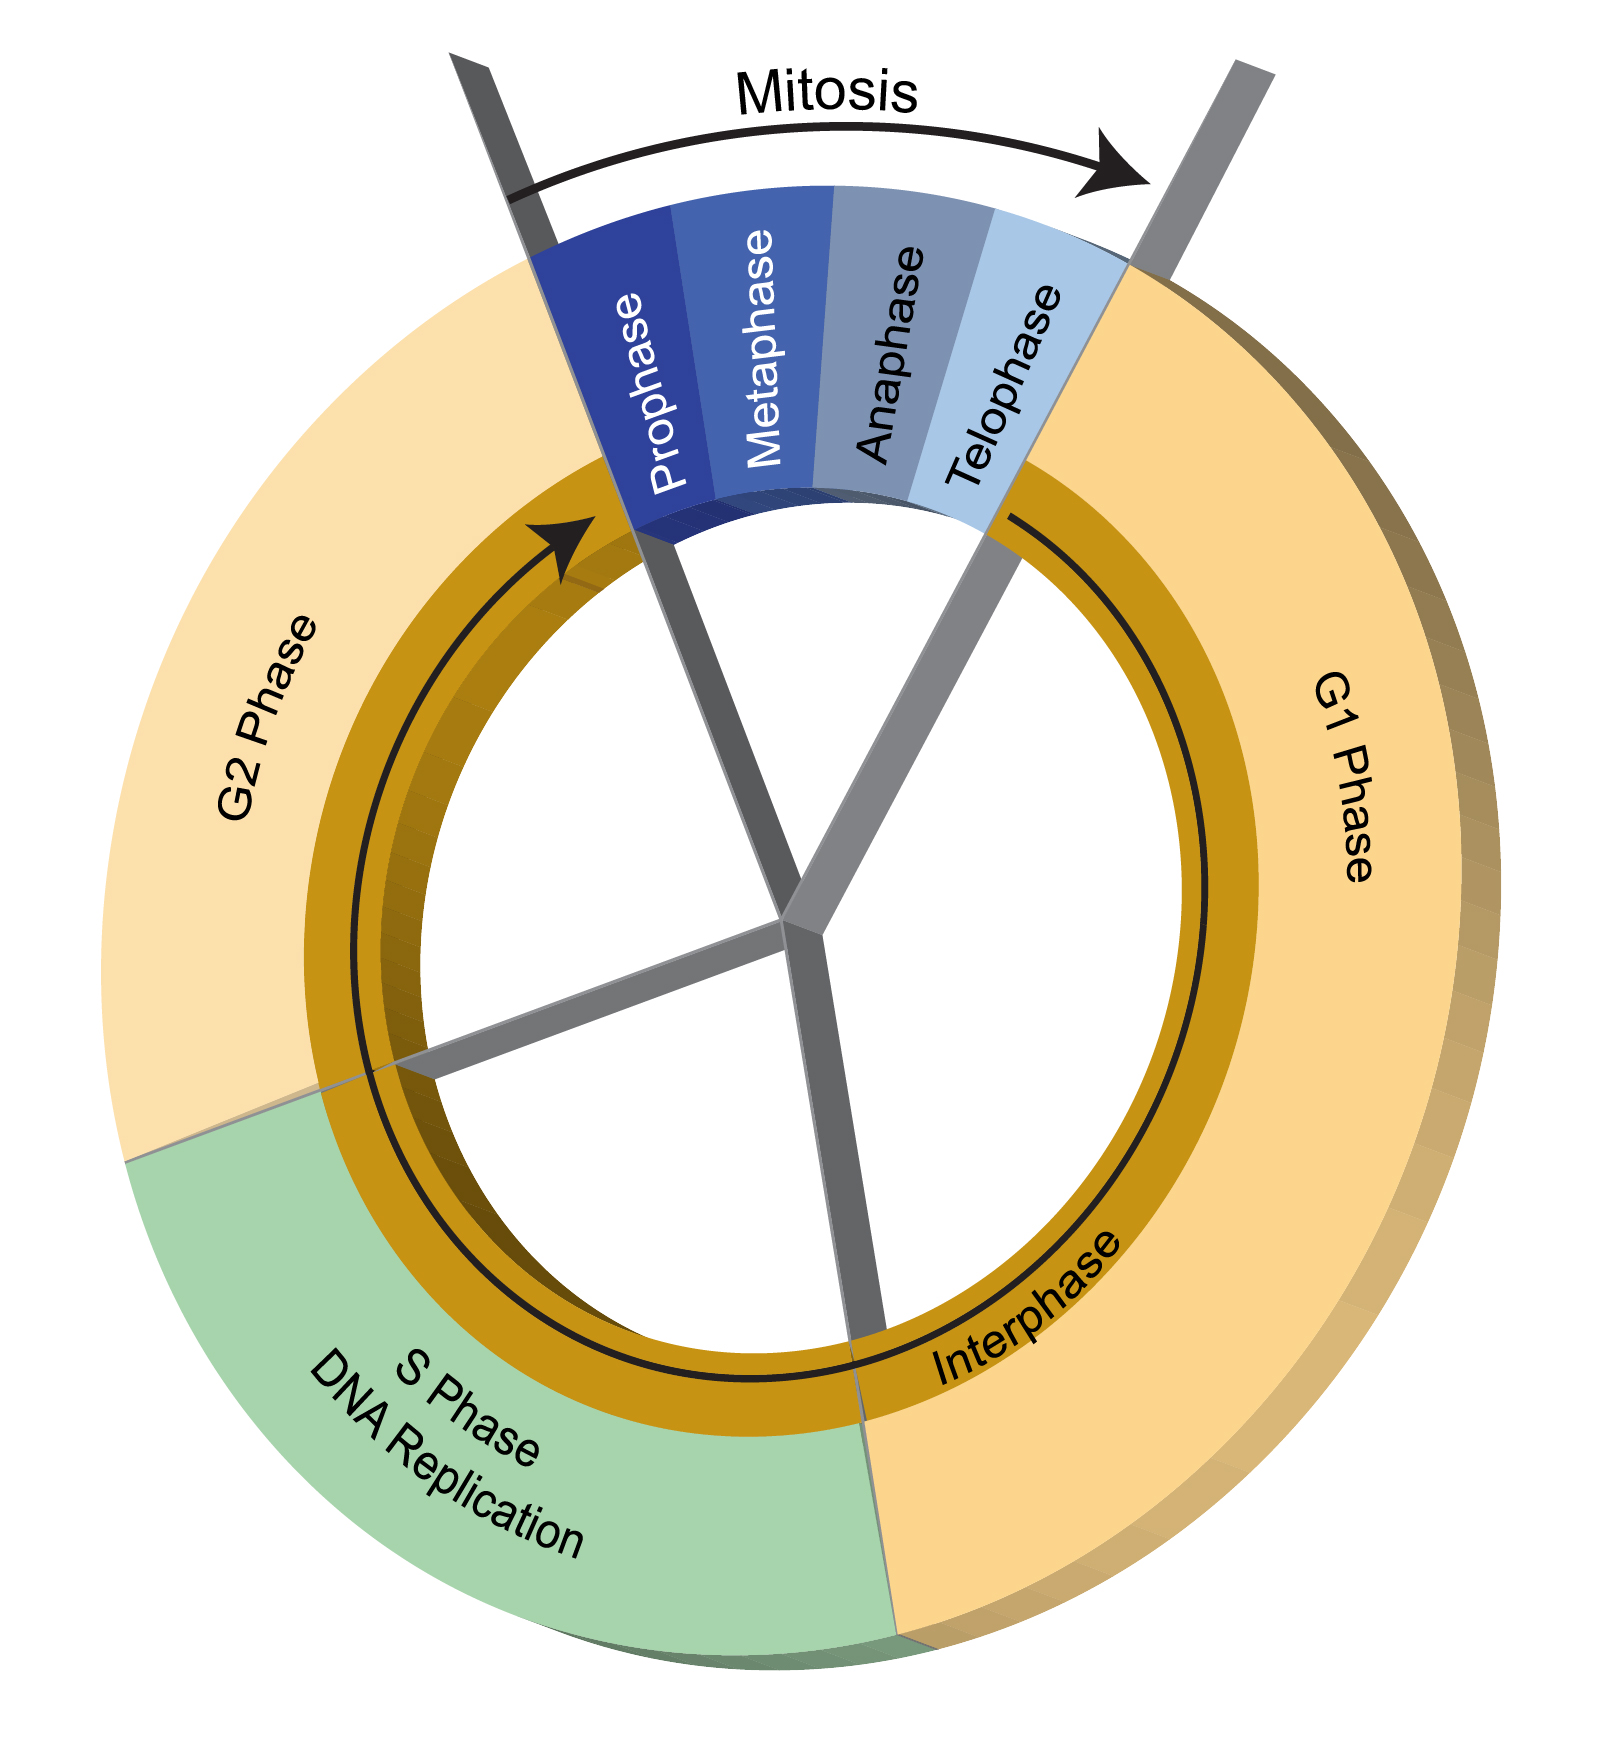
\includegraphics[width=7cm]{Cell_cycle}
	\caption{ چرخه زندگی سلول}
	\label{figure:cellCycle}
\end{wrapfigure}

چرخه زندگی سلول دارای دو بخش اصلی است:
\begin{itemize}
\item اینترفاز
\footnote{\lr{Interphase}}
که طی آن سلول رشد می‌کند و آماده تقسیم می‌شود.
\item میتوتیک فاز
\footnote{\lr{Mitotic (M) phase}}
که طی آن سلول تقسیم می‌شود.
\end{itemize}

اینترفاز خود شامل سه مرحله است:
\begin{description}
\item[\lr{$ G_{1} $ Phase}]
طی این مرحله سلول رشد می‌کند و بزرگ می‌شود.
\item[\lr{$ S $ Phase}]
در این مرحله همانندسازی
\lr{DNA}
رخ می‌دهد.
\item[\lr{$ G_{2} $ Phase}]
طی این مرحله نیز سلول رشد می‌کند. همچنین اندامک‌های لازم همانندسازی می‌کنند و شرایط برای تقسیم سلولی مهیا می‌شود.
\end{description}

میتوتیک فاز نیز خود از دو مرحله تشکیل شده است:
\begin{itemize}
\item میتوز
\footnote{\lr{Mitosis}}
\item سیتوکینز
\footnote{\lr{Cytokinesis}}
\end{itemize}

\bigskip
\bigskip
\bigskip
میتوز خود از چهار مرحله تشکیل شده است:

\begin{figure}[h]
	\centering 
	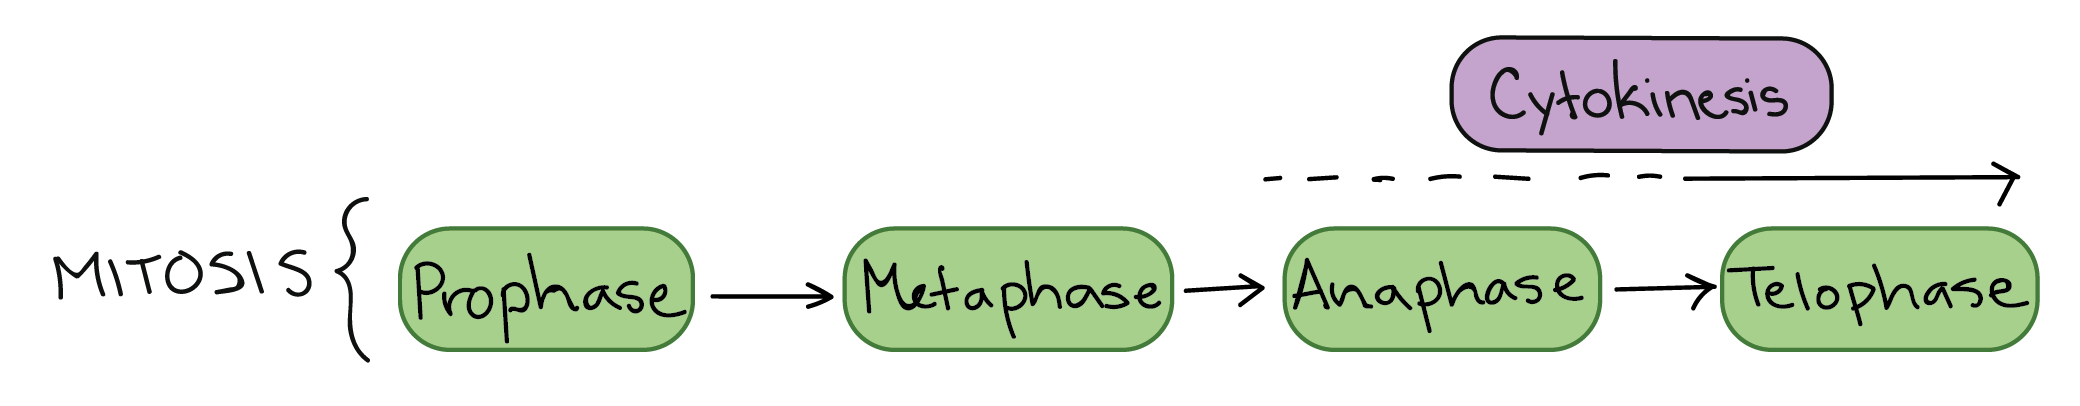
\includegraphics[width=10cm]{Steps_of_mitosis}
\end{figure}

\begin{description}
\item[\lr{Prophase}]
در این مرحله رشته‌های کروماتینی ضخیم، کوتاه و قابل رؤیت می‌شوند. پوشش هسته ناپدید می‌شود و با دور شدن سانتریول‌ها از یکدیگر دوک شکل می‌گیرد.

\begin{figure}[h]
	\centering
	\subfloat[]{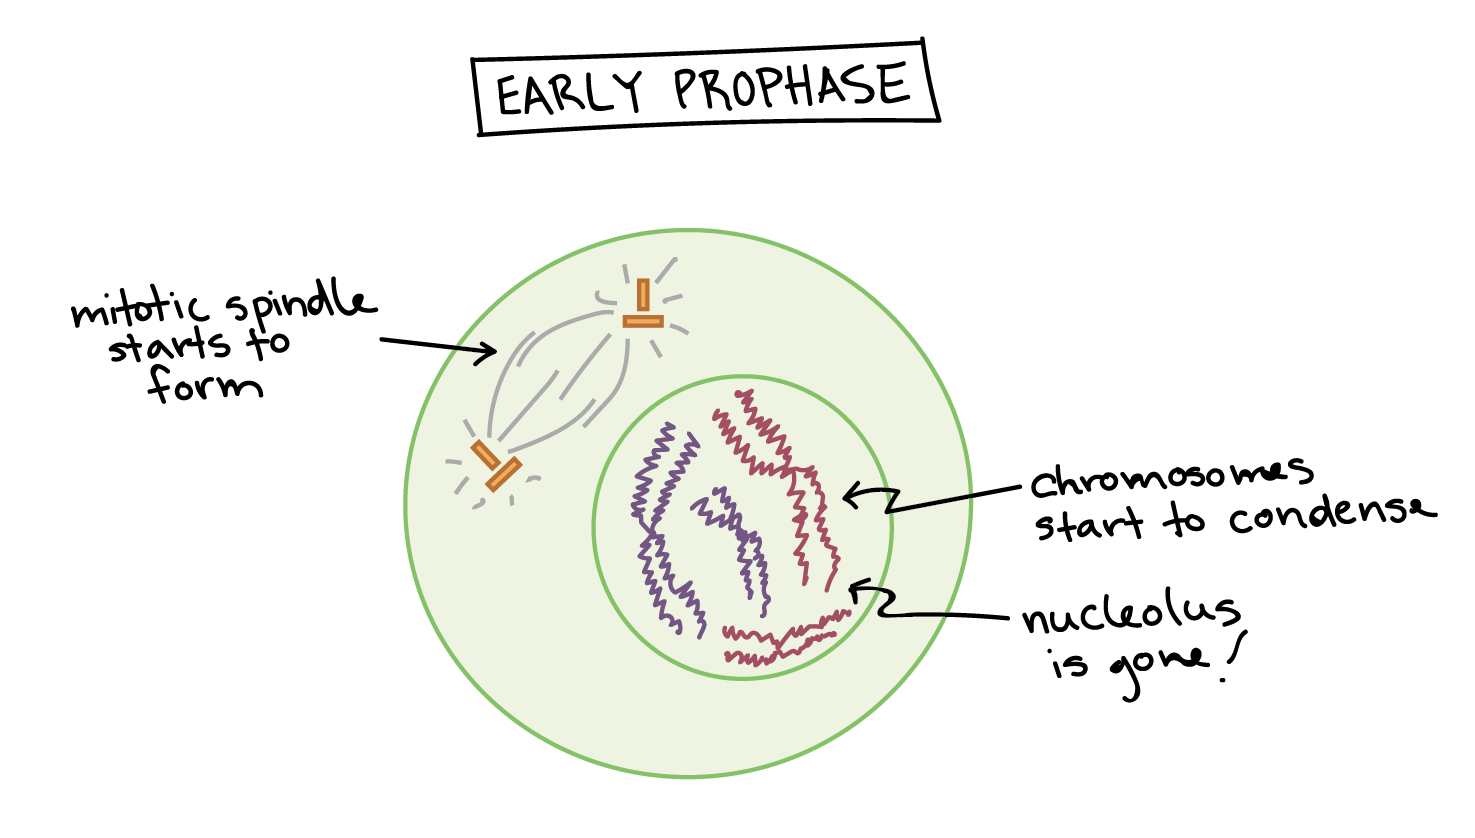
\includegraphics[width=7cm]{Early_prophase}}
	\subfloat[]{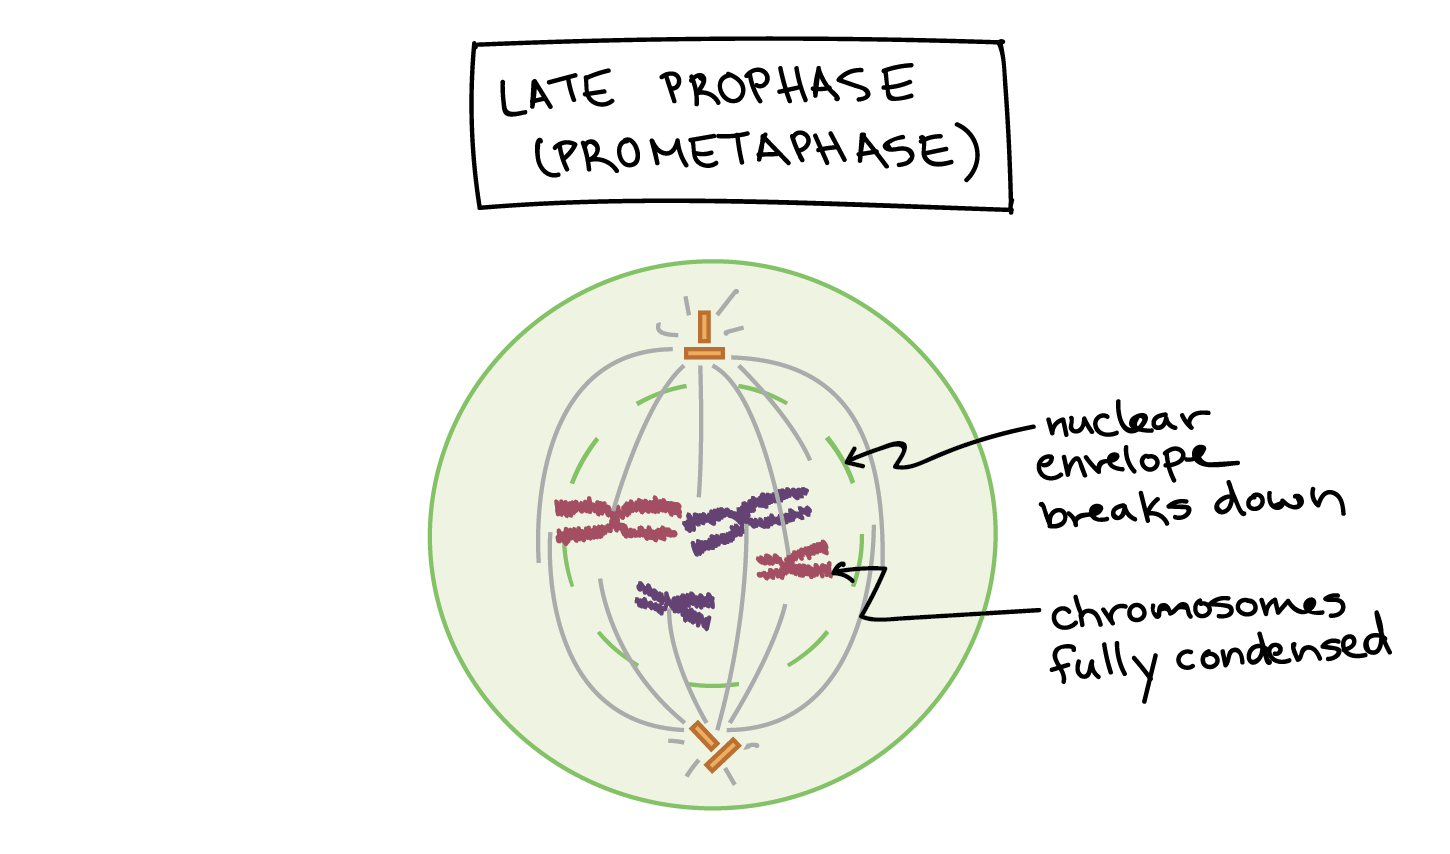
\includegraphics[width=7cm]{Late_prophase}}
\end{figure}

\pagebreak
\item[\lr{Metaphase}]
متا به معنی وسط است.
در متافاز کروموزوم‌ها به سمت وسط سلول حرکت می‌کنند و در سطح استوایی سلول ردیف می‌شوند. در متافاز دو کروماتید هر کروموزوم حداکثر فشردگی را دارند.

\begin{figure}[h]
	\centering
	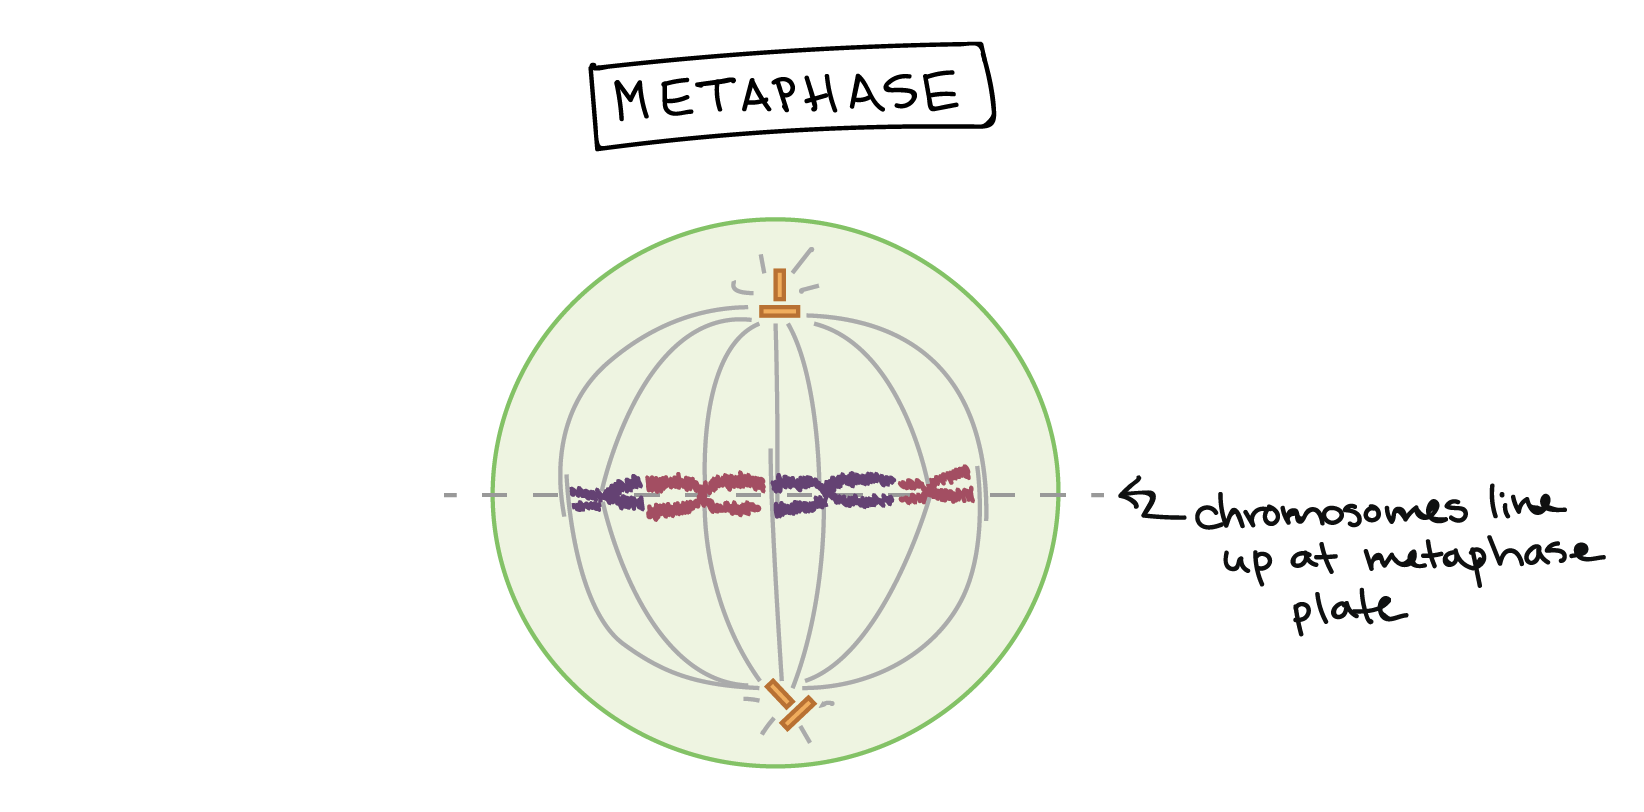
\includegraphics[width=9cm]{Metaphase}
\end{figure}

\item[\lr{Anaphase}]
طی آنافاز کروماتید‌های خواهری از هم جدا می‌شوند و با کوتاه شدن رشته‌های دوک به سمت قطب کشیده می‌شوند.

\begin{figure}[h]
	\centering
	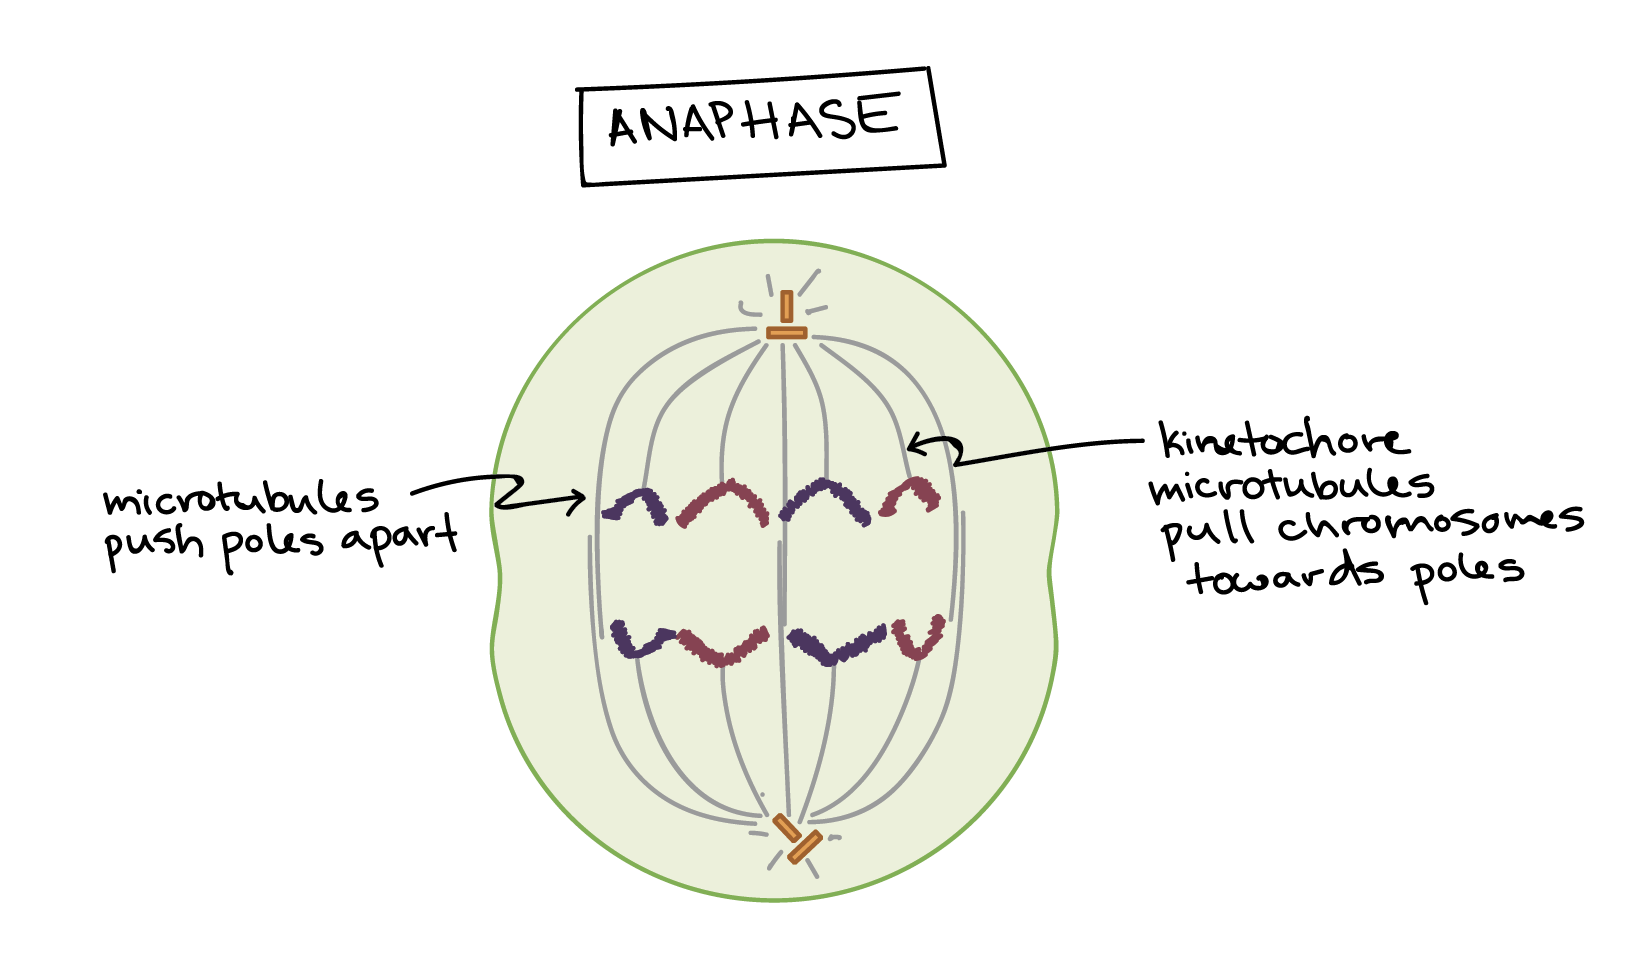
\includegraphics[width=9cm]{Anaphase}
\end{figure}

\item[\lr{Telophase}]
در هر دو قطب پوشش هسته کروموزوم‌ها را احاطه می‌کند. کروموزوم‌ها به مرور از حالت فشردگی خارج می‌شوند. رشته دوک از بین می‌رود. 

\begin{figure}[h]
	\centering
	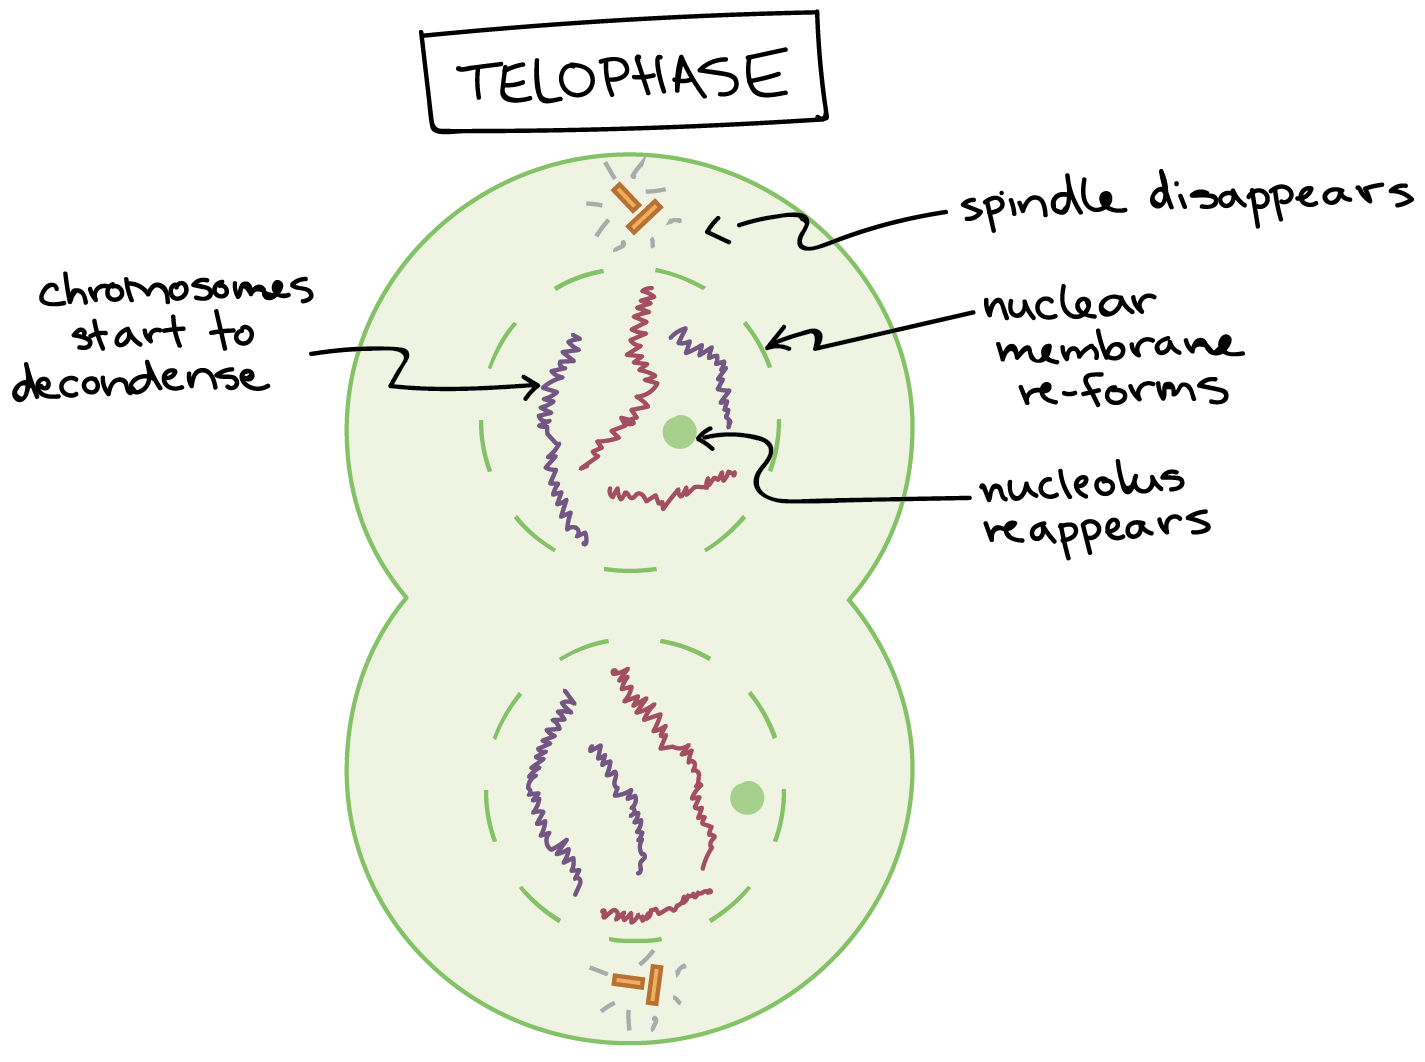
\includegraphics[width=7.5cm]{Telophase}
\end{figure}

\end{description}

\pagebreak
طی سیتوکینز غشا سلول مادری به دو قسمت تقسیم می‌شود و دو سلول دختری کامل می شوند. در سلول‌های جانوری و دیگر سلول‌هایی که دیواره ندارند، طی سیتوکینز، کمربندی از رشته‌های پروتئینی در میان سلول شکل می‌گیرد که با تنگ شدن آن سلول به دو نیمه تقسیم می‌شود. در سلول‌های گیاهی وزیکول‌هایی که توسط دستگاه گلژی ساخته شده‌اند به میانه سلول حرکت می‌کنند و در آنجا به یک دیگر می‌پیوندند و صفحه‌ای را پدید می‌آورند. این صفحه در واقع دیواره‌ای است که با غشا احاطه شده است.

\begin{figure}[h]
	\centering
	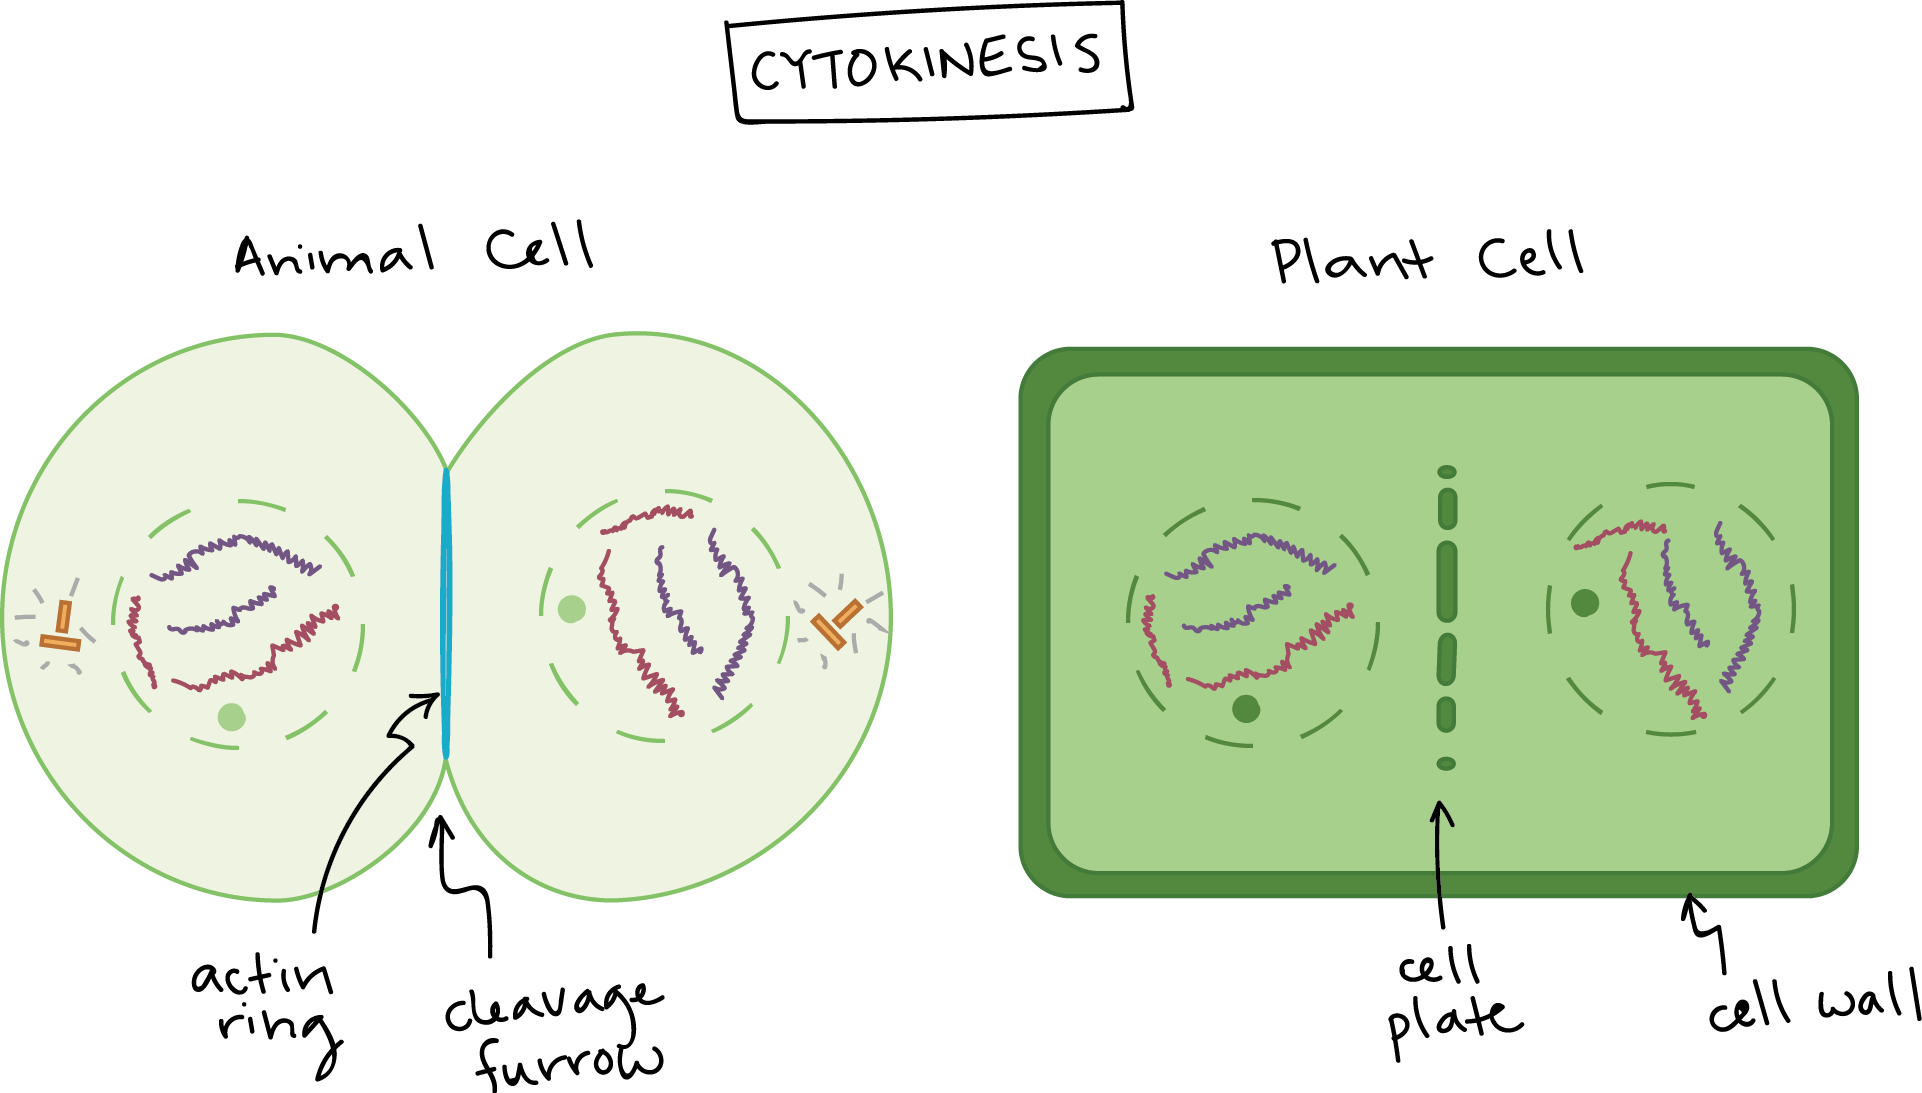
\includegraphics[width=10cm]{Cytokenesis}
\end{figure}

\pagebreak
\subsubsection{تقسیم سلولی میوز\protect\footnote{\lr{Meiosis}}}

تقسیم میتوز سلول‌های دختری ایجاد می‌کند که عینا شبیه به سلول مادر هستند. این تقسیم استفاده‌های مختلفی دارد به عنوان مثال هنگام رشد یا ترمیم زخم. اما میوز تنها با یک هدف استفاده می‌شود و آن تولید گامت
\footnote{\lr{Gamete}}
(سلول جنسی و یا اسپرم
\footnote{\lr{Sperm}}
 و تخمک
 \footnote{\lr{Egg}}
 )
است. با تقسیم میوز سلول‌های دختري به وجود می‌آید که دقیقا نیمی از کروموزوم‌های مادری را دارند.
در انسان، میوز، سلول دیپلوئیدی
\footnote{\lr{Diploid}}
را به دو سلول هاپلوئیدی
\footnote{\lr{Haploid}}
تقسیم می‌کند.

تقسیم میوز از بسیاری جهات همانند تقسیم میتوز است. با این حال تقسیم میوز پیچیده‌تر است چرا که علاوه براین که همانند تقسیم میتوز باید کروماتید‌های خواهری
\footnote{\lr{Sister chromatids}}
هر کروموزوم را جدا کند، میبایست کروموزوم‌های همتا (هومولوگ)
\footnote{\lr{homologous chromosomes}}
را نیز از هم جدا کند.

تقسیم سلولی میوز در دو مرحله انجام میگیرد:
\begin{itemize}
\item میوز
\RN{1}
:
جدا کردن کروموزوم‌های همتا
\item میوز
\RN{2}
:
جدا کردن کروماتید‌های خواهری
\end{itemize}

قبل از شروع تقسیم میوز همانند تقسیم میتوز، سلول وارد مرحله اینترفاز می‌شود. در مرحله
$ G_{1} $
سلول رشد می‌کند. در مرحله
$ S $
کروموزوم‌ها همانندسازی می‌کنند.
در مرحله
$ G_{2} $
شرایط لازم برای تقسیم فراهم می‌شود.


\begin{description}
\item[\lr{Prophase \RN{1}}]
\begin{itemize}
\item[]
\item کروموزوم‌های مضاعف شده فشرده و قابل رؤیت می‌شوند.
\item غشای هسته تجزیه می‌شود.
\item کروموزوم‌های همتا عمل 
\lr{Cross over}
را انجام می‌دهند.

\begin{figure}[htbp]
	\centering
	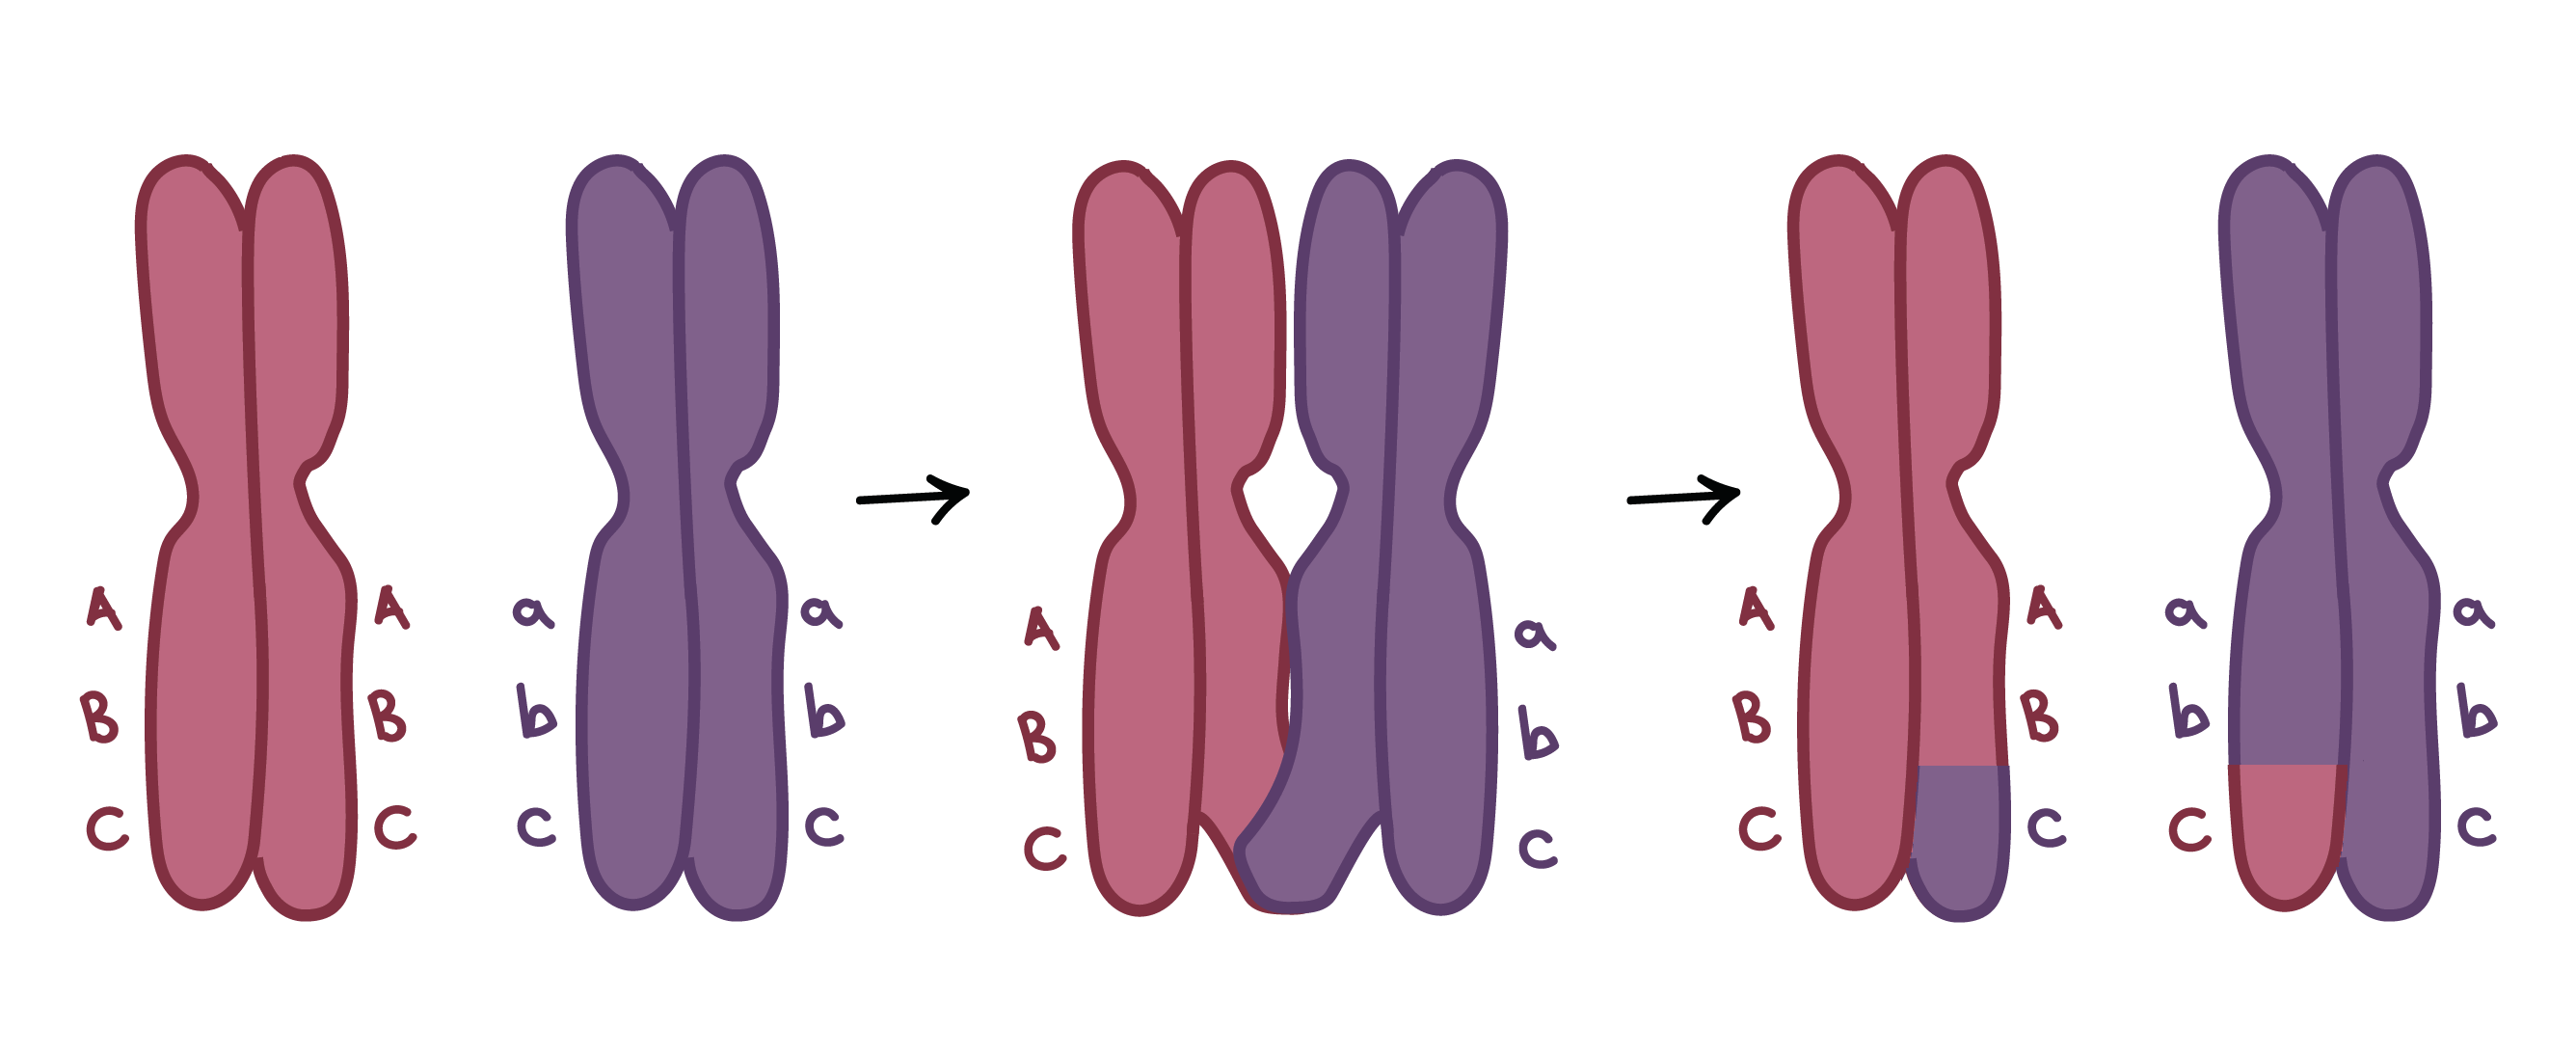
\includegraphics[width=11cm]{Cross_over}
\end{figure}

\item کروموزوم‌های همتا که هر یک دو کروماتیدی هستند از طول کنار یک دیگر قرار می‌گیرند و ساختاری را به وجود می‌آورند که تتراد 
\footnote{\lr{Tetrad}}
نام دارد. در واقع در
\lr{Cross over}
نیز کروموزوم‌ها به همین صورت هستند اما در تصویر قبل برای سادگی این طور نمایش داده شده است. شکل
\ref{figure:HomologuesChromosomes}
را مشاهده کنید. بیش‌ از یک
\lr{Cross over}
هم اتفاق می‌افتد حتی تا
$ 25! $
.
نقاطی که در آن‌ها
\lr{Cross over}
اتفاق می‌افتد کم و بیش تصادفی هستند.


\begin{figure}[htbp]
	\centering 
	\includegraphics[width = 6cm]{Homologues_chromosomes}
	\caption{کروموزوم‌های همتا که در مرحله پروفاز
	کنار هم قرار گرفته اند}
	\label{figure:HomologuesChromosomes}
\end{figure}

\end{itemize}
\item[\lr{Metaphase \RN{1}}]
\begin{itemize}
\item[]
\item تتراد‌ها به وسیله رشته‌های دوک در سطح استوایی سلول ردیف می‌شوند.
\item ترتیب کروموزوم‌های همتا تصادفی است و به همین علت گامت‌هایی با اطلاعات ژنتیکی متفاوت ایجاد می‌شوند.
\end{itemize}
\item[\lr{Anaphase \RN{1}}]
\begin{itemize}
\item[]
\item در این مرحله کروموزوم‌های همتا از یکدیگر جدا میشوند و هر یک به سمت قطب کشیده‌ می‌شوند.
\end{itemize}

\pagebreak
\item[\lr{Telophase \RN{1}}]
\begin{itemize}
\item[]
\item رشته‌های دوک از بین می‌روند.
\item در بعضی از سلول‌ها کروموزوم‌ها را پوشش هسته احاطه می‌کند اما در بعضی دیگر این کار انجام نمی‌شود چرا که سلول وارد تقسیم بعدی می‌شود.
\item در هر یک از هسته‌ها عدد جنسی نصف شده است چرا که از هر کروموزوم همتا فقط یکی وجود دارد.
\end{itemize}
\end{description}

\noindent
میوز
\RN{2}
همانند تقسیم میتوز است:
\begin{description}
\item[\lr{Prophase \RN{2}}]
\begin{itemize}
\item[]
\item غشای هسته تجزیه می‌شود.
\item رشته‌های دوک تشکیل می‌شوند.
\end{itemize}
\item[\lr{Metaphase \RN{2}}]
\begin{itemize}
\item[]
\item کروموزوم‌ها به وسیله رشته‌های دوک در سطح استوایی سلول ردیف می‌شوند.
\end{itemize}
\item[\lr{Anaphase \RN{2}}]
\begin{itemize}
\item[]
\item در این مرحله کروماتید‌های یک کروموزوم از یکدیگر جدا میشوند و هر یک به سمت قطب کشیده‌ می‌شوند.
\item در این مرحله برخلاف میتوز از هر کروموزوم‌ همتا فقط یکی وجود دارد.
\end{itemize}
\item[\lr{Telophase \RN{2}}]
\begin{itemize}
\item[]
\item رشته‌های دوک از بین می‌روند.
\item کروموزوم‌ها را پوشش هسته احاطه می‌کند.
\end{itemize}
\end{description}

\begin{figure}[htbp]
	\centering
	\includegraphics[width=12cm]{Meiosis_one}
	\includegraphics[width=12cm]{Meiosis_two}
	\caption{میوز
	\RN{1}
	و
	میوز
	\RN{2}}
\end{figure}

\pagebreak
\subsubsection{میوز در انسان}

همان طور که در شکل
\ref{figure:spermatogenesis}
مشاهده می‌کنید تقسیم میوز در جنس نر اسپرم‌های با اندازه مساوی ایجاد می‌کند اما در نوع ماده اینگونه نیست در واقع در هر دو مرحله از میوز تقریبا تمام سیتوپلاسم به یکی از دو سلول دختر منتقل می‌شود در نتیجه در انتها تنها یک سلول تخمک ایجاد می‌شود. سایر سلول‌های دختر به دلیل نداشتن سیتوپلاسم از بین می‌روند.

نکته دیگر درمورد انسان این است که در جنس نر اسپرم‌ها در تمام طول زندگی به وجود می‌آیند اما تخمک‌ها از بدو تولد در تخمدان هستند و بعد از این دیگر تخمکی ایجاد نمی‌شود. این نکته تخمک‌ها از ابتدا در رحم هستند باعث می‌شود که با بالاتر رفتن سن در جنس ماده احتمال آسیب دیدن آنها نیز بیشتر شود.

\begin{figure}[htbp]
	\centering
	\includegraphics[width=9cm]{spermatogenesis_oogenesis}
	\caption{تولید اسپرم و تخمک}
	\label{figure:spermatogenesis}
\end{figure}

\subsubsection{کروموزوم‌های جنسی}
در انسان 23 جفت کروموزوم وجود دارد. از این 23 جفت کروموزوم 22 جفت غیر جنسی است که به آنها
\lr{autosome}
می‌گویند
و هر جفت از این 22 جفت نسبت به هم
\lr{Homologous}
هستند اما کروموزوم‌های جنسی
\footnote{\lr{sex chromosomes}}
 ممکن است
\lr{Homologous}
باشند یا نباشند. به عنوان مثال در انسان جنس نر دارای کروموزوم‌های جنسی $ X $
و
$ Y $
است که نسبت به هم همولوگ نیستند اما در جنس ماده کروموزوم‌های جنسی
هر دو
$ X $
هستند که همولوگ می‌باشند.
به جنس ماده
\lr{Homogametic}
می‌گویند چرا که تنها یک نوع گامت از نظر کروموزوم جنسی تولید می‌کند و به جنس نر
\lr{Heterogametic}
می‌گویند چرا که از نظر جنسی دو نوع گامت تولید می‌کند.

\pagebreak
\subsection{سنترال دوگما\protect\footnote{\lr{Central dogma}}}

\begin{figure}[htbp]
	\centering
	\includegraphics[width=12cm]{khan_central_dogma}
	\caption{فرايند
	\lr{Cenral dogma}}
	\label{figure:CentralDogma}
\end{figure}

هر سلولی چه از نوع یوکاریوتی باشد و چه از نوع پروکاریوتی دارای فرآیند سنترال دوگما است که طی آن اطلاعات ژنتیکی به پروتئین تبدیل می‌شود.
طی این فرآیند ابتدا از روی ماده‌ژنتیکی مولکول
\lr{RNA}
ساخته می‌شود سپس این مولکول‌ها به ریبوزوم رفته و از روی آن‌ها پروتئین ساخته می‌شود.
همان طور که در شکل
\ref{figure:CentralDogma}
مشاهده می‌شود این فرآیند شامل دو مرحله است.

\subsubsection{ژن}
هر بخشی از
\lr{DNA}
که از روی آن عمل رونویسی انجام بگیرد ژن نام دارد.

\begin{figure}[htbp]
\centering
\includegraphics[width=12cm]{Gene_regions}
\end{figure}

\noindent
یک نکته که باید به آن توجه کرد این است که در شماره گذاری نوکلئوتید‌های یک ژن عدد صفر وجود ندارد.

\noindent
ژن دارای نواحی است که در رونویسی آن نقش ایفا می‌کنند از جمله:
\begin{itemize}
\item \lr{Promoter}
که در ناحیه بالادستی
\footnote{\lr{upstream}}
ژن قرار دارد.
\item \lr{Terminator}
که در ناحیه پایین‌دستی
\footnote{\lr{downstream}}
ژن قرار دارد.
\end{itemize}

\noindent
یکی از کارهایی که محققان انجام می‌دهند این است که این نواحی مهم را پیشبینی ‌‌کنند. که در واقع با این کار ژن‌ها و عمکرد سلول مشخص می‌شود.

\pagebreak
\subsubsection{رونویسی\protect\footnote{\lr{Transcription}}}
برای اینکه سلول بتواند از روی ژن‌های خود پروتئین بسازد ابتدا نیاز است که به تولید
\lr{mRNA}
\footnote{\lr{messenger RNA}}
بپردازد. این کار مزایای بسیاری دارد. به عنوان مثال وقتی که از روی یک ژن یک
\lr{mRNA transcript}
ساخته می‌شود این
\lr{mRNA transcript}
می‌تواند بار‌ها مورد استفاده قرار گیرد و از روی آن پروتئین ساخته شود در نتیجه به افزایش سرعت بیان ژن کمک می‌شود. از طرفی در سلول‌های یوکاریوتی ماده‌ژنتیکی در هسته قرار دارد درحالی که ریبوزوم‌ها که کارخانه تولید پروتئین هستند درون سیتوزول قرار دارند در نتیجه سلول مجبور است که از یک مولکول واسطه یعنی
\lr{mRNA}
استفاده کند.

به این عمل که طی آن از روی ژن
\lr{mRNA}
ساخته می‌شود رونویسی گفته می‌شود. رونویسی در سلول یوکاریوتی و پروکاریوتی متفاوت است چرا که در سلول یوکایوتی اگر
\lr{mRNA}
به صورت خام وارد سیتوزول شود توسط آنزیم‌ها تجزیه میشود. اما در سلول‌های پروکاریوتی پیش‌پردازشی انجام نمی‌شود چرا که ماده‌ژنتیکی در سیتوزول قرار دارد.

توجه شود که در سلول‌های یوکاریوتی بعضی از پروتئین‌ها داخل هسته ساخته می‌شوند. این نکته در کارهای محاسباتی اهمیت دارد چرا که یکی از کار‌های محاسباتی این است که از روی سیگنال تشخیص داده شود که پروتئین مربوطه داخل هسته ساخته می‌شود و یا خارج از آن.

\begin{figure}[htbp]
	\centering
	\includegraphics[width=14cm]{TranscriptionEucaryoticAndProcayotic}
\end{figure}

اصلی‌ترین آنزیم در رونویسی
\lr{RNA polymerase}
است که نحوه عمل آن مانند
\lr{DNA polymerase}
است با این تفاوت که
\lr{RNA polymerase}
از روی
\lr{template strand}
مولکول
\lr{mRNA}
می‌سازد.
\lr{RNA polymerase}
،
\lr{mRNA}
را در جهت
$ 5^\prime $
به
$ 3^\prime $
می‌سازد و هر نوکلئوتید را به سر
$ 3^\prime $
\lr{strand}
اضافه می‌کند.

\lr{RNA polymerase}
ها مولکول‌های بزرگی هستند که از چندین ریزعضو
\footnote{\lr{subunit}}
تشکیل شده‌اند. یوکاریوت‌ها دارای سه نوع
\lr{RNA polymerase}
هستند:
\RN{1}
,
\RN{2}
و
\RN{3}
.
هر یک از این‌ها گروه خاصی از ژن‌ها را رونویسی می‌کنند.
نوع
\RN{1}
ژن‌های مربوط به
\lr{rRNA}
ها را رونویسی می‌کند.
نوع
\RN{2}
مربوط به
\lr{mRNA}
ها و بعضی
\lr{snRNA}
ها است و نوع
\RN{3}
ژن‌های مربوط به
\lr{tRNA}
ها
،
\lr{5S RNA}
ها و
\lr{snRNA}
ها را رونویسی می‌کند.
گیاهان دو نوع
\lr{RNA polymerase}
دیگر نیز دارند و آن نوع
\RN{4}
و
\RN{5}
است که در سنتز
انواع خاصی از
\lr{RNA}
های کوچک کاربرد دارند.
\cite{StagesOfTranscription}

\begin{figure}[htbp]
\centering
\includegraphics[width=12cm]{RNA_Polymerase}
\end{figure}

\pagebreak
\noindent
رونویسی شامل سه مرحله است:
\begin{itemize}
\item آغاز
\footnote{\lr{initiation}}
\item طویل شدن
\footnote{\lr{elongation}}
\item پایان
\footnote{\lr{termination}}
\end{itemize}

\begin{figure}[htbp]
\centering
\includegraphics[width=12cm]{TranscriptionCycle}
\caption{رونویسی در باکتری}
\end{figure}

\pagebreak
\subsubsection{آغاز رونویسی\protect\footnote{\lr{Transcription initiation}}}
برای شروع همانندسازی
\lr{RNA polymerase}
باید به ژن متصل شود. این اتصال در ناحیه‌ای به نام
\lr{promoter}
انجام می‌شود.

\begin{figure}[htbp]
\centering
\includegraphics[width=12cm]{Promoter}
\end{figure}

\noindent
هر ژن (و یا گروهی از ژن‌ها که در باکتری با هم رونویسی می‌شوند)
\cite{StagesOfTranscription}
دارای
\lr{promoter}
خاص خود هستند.

باکتری‌ها می‌توانند ساختاری به نام
\lr{operon}
داشته باشند که شامل چند ژن است که تنها یک ناحیه
\lr{promotor}
دارند و همه این ژن‌ها همزمان بیان می‌شوند. بین از رونویسی
\lr{mRNA}
تقسیم می‌شود و هر تکه مربوط به یک ژن است.
یوکاریوت‌ها فاقد چنین ساختاری هستند.

\begin{figure}[htbp]
\centering
\includegraphics[width=10cm]{operon}
\end{figure}

\noindent
به طور کلی دو دسته
\lr{promoter}
داریم:
\begin{description}
\item[\lr{constitutive}]
این
\lr{promotor}
ها مخصوص ژن‌هایی هستند که همیشه بیان میشوند به عنوان مثال
ژن‌های مربوط به
\lr{tRNA}
،
\lr{rRNA}
،
\lr{ribosomal proteins}
و
\lr{RNA polymerase}
دارای این نوع
\lr{promotor}
هستند.
\item[\lr{inducible}]
مربوط به ژن‌هایی هستند که در شرایط خاصی بیان می‌شوند. اکثر ژن‌ها دارای این نوع
\lr{promotor}
هستند.
\end{description}

\lr{transcription factor}
ها عناصری هستند که به نشستن
\lr{RNA polymerase}
روی پرومتر کمک می‌کنند. به عنوان مثال اکثر ژن‌های باکتری با کمک زیرواحد
$\sigma^{70}$
می‌توانند شروع به رونویسی کنند. و چون
$\sigma^{70}$
همیشه در سلول وجود دارد، این ژن‌ها زیاد بیان می‌شوند. حال اگر ژنی از نوع
\lr{inducible}
باشد از زیرواحد‌های دیگری مانند
$\sigma^{54}$
کمک می‌گیرند.

\pagebreak
علاوه بر
\lr{TF}
ها پروتئین‌های دیگری به نام
\lr{activator}
وجود دارند که در منطقه بالادستی ژن می‌نشینند و برای
\lr{RNA polymerase}
کشش ایجاد می‌کنند. سلول از این پروتئین‌هابرای افزایش بیان ژن استفاده می‌کند.

\begin{figure}[htbp]
\centering
\includegraphics[width=12cm]{GeneActivator}
\end{figure}

\begin{figure}[htbp]
\centering
\includegraphics[width=12cm]{Enhancer}
\caption{\lr{Transcription initiation by
RNA polymerase \RN{2} in a eucaryotic cell}}
\label{figure:enhancer}
\end{figure}

در شکل
\ref{figure:enhancer}
مشاهده می‌شود که یک
\lr{activator}
می‌تواند در منطقه بسیار بالاتر از ژن بنشیند. در این حالت ساختار سه بعدی
\lr{DNA}
در جذب کردن
\lr{RNA polymerase}
دخیل است.

\begin{figure}[htbp]
\centering
\includegraphics[width=12cm]{AlternateSigmaFactorUsage}
\caption{\lr{n}
به معنای هر نوکلئوتیدی است. توالی‌های نشان‌داده شده همیشه به این صورت نیستند و ممکن است در یک گونه جهش‌هایی صورت گرفته باشد.}
\label{figure:alternateSigma}
\end{figure}

همانطور که در شکل
\ref{figure:alternateSigma}
مشاهده می‌کنید در شرایط گوناگون باکتری
\lr{TF}
های متفاوتی تولید می‌کند که این به نوبه خود باعث فعال شدن ژن‌های متفاوتی می‌شود که محصولات متناسب با محیط تولید می‌کنند. نکته دیگر اینکه به عنوان مثال هر چقدر ناحیه
$-10$
به
\lr{TTGACA}
شبیه‌تر باشد کشش آن برای فاکتور
$\sigma$
بیشتر می‌شود. گاهی اوقات ممکن است جهش‌هایی در این منطقه ایجاد شود که موجب کاهش کشش شوند. به عنوان مثال ممکن است جهش‌های ایجاد شده در ژنوم فردی او را مجبور کند تا مقدار زیادی مواد ویتامینی بخورد تا ویتامین‌ها به سمت یک ناحیه کشش پیدا کنند.

\pagebreak
سلول علاوه بر اینکه می‌تواند با تولید
\lr{activator}
میزان بیان یک ژن را افزایش دهد، همچنین می‌تواند با تولید پروتئین‌هایی به نام
\lr{repressor}
بیان یک ژن را کاهش دهد.
\lr{repressor}
ها مانع از نشتن
\lr{RNA polymerase}
در
\lr{promotor}
می‌شوند.

\begin{figure}[htbp]
\centering
\includegraphics[width=10cm]{Repressor}
\end{figure}

\pagebreak
\subsubsection{پرومتر در باکتری\protect\footnote{\lr{Promoters in bacteria}}}

\begin{wrapfigure}[12]{l}{10cm}
\centering
\includegraphics[width=10cm]{BacteriaPromoter}
\end{wrapfigure}

یکی از
\lr{promoter}
های
\lr{typical}
در باکتری دارای دو
\lr{DNA sequence}
مهم است که عنصر
\footnote{\lr{element}}
$ -10 $
و
$ -35 $
نام دارند.
این نامگذاری به این علت است که این ناحیه‌ها به ترتیب
$ 10 $
و
$ 35 $
نوکلئوتید از نقطه شروع رونویسی عقب‌تر هستند. این دنباله‌ها کمک می‌کنند که
\lr{RNA polymerase}
در نقطه شروع رونویسی قرار گیرد و نیز جهت آن را تنظیم می‌کنند.

بعد از آنکه
\lr{RNA polymerase}
به رشته متصل شد، می‌تواند رشته
\lr{DNA}
را از هم باز کند. این باز کردن در ناحیه عنصر
$ -10 $
صورت میگیرد. عنصر
$ -10 $
یک ناحیه
\lr{AT rich}
است و در نتیجه به آسانی باز می‌شود.
\cite{StagesOfTranscription}

\begin{figure}[htbp]
\centering
\includegraphics[width=14cm]{Prokaryotic_gene}
\caption{ژن باکتری}
\label{figure:prokaryoticGin}
\end{figure}

برای آنکه
\lr{RNA polymerase}
بتواند سریعتر به ناحیه پرومتر متصل شود پروتئین‌های کوچکتری به نام
\lr{transcription factor}
پرومتر را شناسایی می‌کنند سپس این فاکتورها
\lr{RNA polymerase}
را به سمت خود می‌کشند. زیر‌واحدی که می‌تواند روی پرومتر باکتری بشیند زیرواحد سیگما نام دارد.

\begin{figure}[htbp]
\centering
\includegraphics[width=9.6cm]{transcription_factor1}
\includegraphics[width=9.6cm]{transcription_factor2}
\end{figure}

همانطور که در شکل
\ref{figure:prokaryoticGin}
مشاهده می‌کنید،
\lr{coding region}
ناحیه است که دقیقا پروتئین از روی آن ساخته می‌شود. اما همانطور که مشاهده می‌کنید قبل و بعد از این ناحیه توالی‌هایی وجود دارد که آنها هم رونویسی می‌شوند درحالی که ترجمه نمی‌شوند. با توجه به اینکه سلول پروکاریوتی هسته ندارد بعد از رونویسی، آنزیم‌ها به
\lr{mRNA}
حمله می‌کنند.
\lr{Antileader}
و
\lr{Antitrailer}
ناحیه‌هایی هستند که از روی آنها
توالی‌های
\lr{Leader}
و
\lr{Trailer}
در
\lr{mRNA}
شکل می‌گیرند.
\lr{Leader}
و
\lr{Trailer}
توالی‌هایی هستند که شکل خاصی به خود می‌گیرند و از
\lr{degradat}
شدن
\lr{mRNA}
جلوگیری می‌کنند.
البته در انتها این
\lr{mRNA}
،
\lr{degradat}
می‌شود اما این ساختار‌ها برای مولکول زمان می‌خرند.
توجه کنید که از روی
\lr{coding region}
ترجمه انجام ‌می‌شود و این قسمت نمی‌تواند به خود شکل بگیرد. برای محافظت از
\lr{coding region}
تعدادی پروتئین به آن می‌چسبند.

نکته‌ی دیگری که در شکل
\ref{figure:prokaryoticGin}
مشخص شده است این است که در ابتدای
\lr{mRNA}
(نه از ابتدای
\lr{coding region}
)
معمولا نوکلئوتید
\lr{A}
یا
\lr{G}
قرار دارد.
توالی مهم دیگری که در ناحیه
\lr{Leader}
قرار دارد،
\lr{Shine-Dalgarno}
است. این توالی با توالی خاصی در
\lr{rRNA}
که در ساختار ریبوزوم به کار می‌رود، مکمل می‌شود. اولین نقطه‌ای از
\lr{mRNA}
که به ریبوزوم متصل می‌شود همین توالی است.
\begin{figure}[htbp]
\centering
\includegraphics[width=12cm]{Shine_dalgarno}
\end{figure}

\noindent
سه نوکلئوتید اول در
\lr{coding region}
،
\lr{AUG}
هستند.
بین ناحیه
$ -10 $
و
$ -35 $
،
$ 16 $
تا
$18$
نوکلئوتید فاصله وجود دارد. اگر این فاصله کم یا زیاد شود زیر واحد سیگما نمی‌تواند در این منطقه بنشیند و در نتیجه رونویسی با مشکل مواجه می‌شود.

\begin{figure}[htbp]
\centering
\includegraphics[width=12cm]{SpaceBetweenLegsInPromoter}
\end{figure}

\begin{figure}[htbp]
\centering
\includegraphics[width=12cm]{EcoliGene}
\caption{در این تصویر ژن‌ها متفاوت 
\lr{Ecoli}
با هم مقایسه شده‌اند.}
\end{figure}

\pagebreak
\subsubsection{پرومتر در یوکاریوت‌ها\protect\footnote{\lr{Promoters in Eukaryot}}}
در یوکاریوت‌ها مانند انسان
\lr{RNA polymerase}
اصلی به صورت مستقیم به رشته
\lr{DNA}
متصل نمی‌شود. ابتدا پروتئین‌های کمکی به نام
\lr{basal (general) transcription factors}
به
\lr{promoter}
 متصل می‌شوند و سپس این فاکتور‌ها
\lr{RNA polymerase}
را به سمت خود می‌کشند.

بسیاری از
\lr{promoter}
های یوکایوتی دنباله‌ای به اسم
\lr{TATA box}
دارند که مانند عنصر
$ -10 $
در باکتری یک ناحیه
\lr{AT rich}
است.
\lr{TATA box}
توسط یکی از
\lr{general transcription factor}
ها شناسایی می‌شود. بعد از اتصال،
این فاکتور باعث می‌شود تا سایر فاکتور‌ها و در نتیجه
\lr{RNA polymerase}
به
\lr{promoter}
متصل شوند.

\begin{figure}[htbp]
\centering
\includegraphics[width=12cm]{HumanPromoter}
\caption{\lr{TATA box}}
\end{figure}

همانطور که قبلا در بخش رونویسی گفته شد در یوکایوت‌ها سه نوع
\lr{RNA polymerase}
وجود دارد. که هر کدام از اینها سیگنال‌های خاصی را در قسمت
\lr{promotor}
ژن شناسایی می‌کنند.

\begin{figure}[htbp]
\centering
\includegraphics[width=12cm]{RnaPolOnePromotor}
\caption{پرومتر مربط به
\lr{RNA polymerase \RN{1}}}
\end{figure}

\begin{figure}[htbp]
\centering
\includegraphics[width=12cm]{RnaPolTowPromotor}
\caption{یک ژن که توسط
\lr{RNA polymerase \RN{2}}
رونویسی می‌شود.}
\end{figure}

\begin{figure}[htbp]
\centering
\includegraphics[width=12cm]{RnaPolThreePromotor}
\caption{دو نوع پرومتر مربوط به
\lr{RNA polymerase \RN{3}}}
\end{figure}

یکی از مسئله‌های مطرح در
\lr{Bioinformatics}
شناسایی سیگنال‌های
\lr{promotor}
برای هر یک از این
\lr{RNA polymerase}
ها است.

علاوه بر
\lr{general transcription factor}
ها
\lr{factor}
های دیگری به نام
\lr{specific transcription factor}
ها در بیان ژن کمک می‌کنند.
\lr{GTF}
ها فاکتور‌هایی هستند که در اکثر ژن‌های یوکاریوتی گیرنده دارند اما ژن علاوه بر آنها به تعدادی
\lr{STF}
نیز نیاز دارد تا بتواند
\lr{RNA polymerase}
را به سمت خود هدایت کند. این
\lr{STF}
بسته به ژن‌ها متفاوت هستند و این راهی است که سلول به وسیله آ‌ن میزان بیان ژن‌های خود را تنظیم می‌کند.بعضی از ژن‌ها همبیان
\footnote{\lr{co-expressed}}
هستند به این معنی که همزمان بیان می‌شوند. علت این امر این است که این ژن‌ها دارای جایگاه
\lr{STF}
یکسانی هستند.

\pagebreak
\subsubsection{طویل شدن\protect\footnote{\lr{elongation}}}

\begin{wrapfigure}[7]{l}{8cm}
\centering
\includegraphics[width=8cm]{Elongation}
\end{wrapfigure}

بعد از اتصال
\lr{RNA polymerase}
به رشته
\lr{DNA}
نوبت به ساخت
\lr{mRNA}
می‌رسد. در مرحله
\lr{e\textcolor{red}{long}ation}
مولکول
\lr{mRNA}
طویل
\lr{(\textcolor{red}{long})}
می‌شود.

ساخت
\lr{mRNA transcript}
از روی
\lr{template strand}
انجام می‌شود. به لحاظ توالی نوکلئوتید‌ها،
\lr{mRNA}
شبیه به
\lr{strand}
دیگر یعنی
\lr{non-template strand}
و یا
\lr{coding strand}
است با این تفاوت که به جای نوکلئوتید
\lr{T}
، نوکلئوتید
\lr{U}
قرار می‌گیرد.

\vspace{2cm}
\begin{figure}[htbp]
\centering
\includegraphics[width=12cm]{ChimicalReactionOfElongation}
\caption{واکنش شیمیایی که طی طویل شدن اتفاق می‌افتد.}
\end{figure}

\begin{figure}[htbp]
\centering
\includegraphics[width=8cm]{RnaPolymerasesInElongation}
\caption{همانطور که در شکل فوق مشاهده می‌کنید یک ژن همزمان توسط چندین
\lr{RNA polymerase}
مورد رونویسی قرار می‌گیرد. در ابتدای ژن
\lr{mRNA}
ها کوتاه هستند اما با نزدیک شدن به انتهای ژن طویل می‌شوند.}
\end{figure}

\pagebreak
\subsubsection{پایان رونویسی در باکتری\protect\footnote{\lr{Termination in bacteria}}}

\begin{wrapfigure}[10]{l}{10cm}
\centering
\includegraphics[width=10cm]{RhoDependentTermination}
\end{wrapfigure}

دو نوع
\lr{termination}
اصلی در باکتری وجود دارد:
\lr{Rho-dependent}
و
\lr{Rho-independent}
.
در
\lr{Rho-dependent termination}
سیگنال خاصی در انتهای ژن وجود دارد که  توالی خاصی را در
\lr{mRNA}
به وجود می‌آورد. این توالی یک
\lr{binding site}
را به وجود می‌آورد که
\lr{Rho factor}
به آن متصل می‌شود.
\lr{Rho factor}
بعد از اتصال به
\lr{mRNA}
به سمت
\lr{RNA polymerase}
حرکت می‌کند و بعد از رسیدن به آن باعث جدا شدن می‌شود.

\vspace{2.7cm}
\begin{wrapfigure}[13]{l}{10cm}
\centering
\includegraphics[width=10cm]{RhoIndependentTermination}
\end{wrapfigure}

در
\lr{Rho-independent termination}
توالی خاصی در انتهای ژن وجود دارد که  غنی از نوکلئوتید‌های
\lr{C}
و
\lr{G}
است.
\lr{mRNA}
ای که از روی این ناحیه رونویسی می‌شود بر روی خود خم می‌شود و ساختاری شبیه به گیره‌ی‌مو
\footnote{\lr{hairpin}}
به وجود می‌آورد.
در
\lr{terminator}
بعد از سیگنال گیره‌ی‌مو ناحیه غنی از نوکلئوتید
\lr{A}
وجود دارد که با نوکلئوتید
\lr{U}
در
\lr{mRNA}
مچ می‌شوند در نتیجه ناحیه‌ای با پیوند سست به وجود می‌آورند که با وجود ساختار گیره‌ باعث جدا شدن
\lr{mRNA}
می‌شوند.

اما چرا سیستم پایان یافتن رونویسی به روش‌های متفاوتی انجام می‌شود؟ یکی از علت‌های آن می‌تواند این باشد که ژن‌های که نوع پایان آن‌ها متفاوت است کارایی خاصی دارند و از مسیر تکاملی متفاوتی نمو پیدا کرده‌اند. سپس در یک موجود گرد هم آمده‌اند.

\begin{figure}[htbp]
\centering
\includegraphics[width=8.5cm]{Hairpin}
\end{figure}

\pagebreak
\subsubsection{محافظت\protect\footnote{\lr{Protection}}}

\begin{wrapfigure}[20]{l}{10cm}
\centering
\includegraphics[width=10cm]{fiveCap}
\end{wrapfigure}

در سلول‌های پروکاریوتی
مولکول
\lr{mRNA}
بعد از رونویسی می‌تواند مورد ترجمه قرار بگیرد اما در سلول‌های یوکاریوتی نیاز است که تعدادی پیش‌پردازش صورت بگیرد. این پیش‌پردازش‌ها دو نوع هستند:
\begin{itemize}
\item محافظت
\item پیوند
\end{itemize} 

اگر مولکول
\lr{mRNA}
بدون محافظت از هسته خارج شود ممکن است در معرض
\lr{degradation}
قرار گیرد.
با توجه به اینکه
\lr{degradation}
از سر مولکول انجام می‌شود، سلول رشته
\lr{mRNA}
را از دو سمت
$ 5^\prime $
و
$ 3^\prime $
محافظت می‌کند. سر
$ 5^\prime $
یک نوکلئوتید
\lr{G}
به سر
$ 5^\prime $
رشته
\lr{mRNA}
وصل می‌شود که به آن کلاه
$ 5^\prime $
\footnote{\lr{$ 5^\prime $ cap}}
گفته می‌شود. با این کار سر
$ 5^\prime $
رشته
\lr{mRNA}
مخفی می‌شود.
به سر
$ 3^\prime $
رشته
\lr{mRNA}
تعداد زیادی نوکلئوتید
\lr{A}
وصل می‌شود که به آن
\lr{poly-A tail}
گفته می‌شود.
این کلاه
$ 5^\prime $
و
\lr{poly-A tail}
سلول را از خطر آنزیم‌های
\lr{exonucleases}
محافظت می‌کنند.
\lr{RNA}
هایی که سر
$ 5^\prime $
آشکار دارند از جمله هدف‌های این آنزیم‌ها هستند.

\vspace{2cm}
کلاه
$ 5^\prime $
به اتصال
\lr{mRNA}
به ریبوزوم نیز کمک می‌کند.
توجه شود که ساختار
\lr{Leader}
و
\lr{Trailer}
در یوکاریوت‌ها نیز وجود دارد و این محافظت‌ها علاوه بر آن است.

\begin{figure}[htbp]
\centering
\includegraphics[width=12cm]{RnaProtection}
\end{figure}

اگر
\lr{poly-A tail}
بیش از حد طولانی شود ممکن است موجب بیماری شود چرا که تجزیه این
\lr{mRNA}
به تعویق می‌افتد و در نتیجه از روی آن بارها پروتئین ساخته می‌شود در حالی که ممکن است بدن به این حجم از این پروتئین نیاز نداشته باشد و خود باعث بروز مشکلات شود.

\pagebreak
\subsubsection{پیوند\protect\footnote{\lr{splicing}}}
هدف از
\lr{splicing}
حذف کردن
\lr{intron}
ها است.
\lr{intron}
ها قسمت‌هایی از رشته
\lr{RNA}
هستند که فاقد اطلاعات درمورد ساخت پرو‌تئین هستند. علت وجود
\lr{intron}
ها به خاطر این است که احتمال جهش روی بخش اصلی ژن کاهش پیدا کند. حذف
\lr{intron}
ها به وسیله یک
\lr{complex}
از آنزیم‌ها به نام
\lr{spliceosome}
انجام می‌شود.
\lr{spliceosome}
مکان
\lr{intron}
ها را شناسایی می‌کند سپس آنها را از رشته
\lr{mRNA}
جدا می‌کند و در نهایت تکه‌های جدا شده
\lr{mRNA}
را به هم می‌چسباند.
قسمت‌هایی از
\lr{mRNA}
که حذف نمی‌شوند
\lr{exon}
ها را تشکیل می‌دهند.
بعضی به
\lr{mRNA}
ای که شامل
\lr{intron}
است
\lr{pre-mRNA}
گویند. و به
\lr{mRNA}
ای که بعد از
\lr{splicing}
به وجود می‌آید
\lr{primary mRNA}
و یا
\lr{mature mRNA}
می‌گویند.

\begin{figure}[htbp]
\centering
\includegraphics[width=12cm]{RnaSplicing}
\end{figure}

جالب است که
\lr{intron}
ها قبل از باکتری‌ها در آرکئا وجود داشته است اما هنگام مشتق شدن در باکتری از بین رفته اما در یوکاریوت‌ها باقی مانده است.

\begin{figure}[htbp]
\centering
\includegraphics[width=17cm]{splicingDetail}
\caption{
\lr{snRNP}
ها همان
\lr{snRNA}
هستند که تعدادی پروتئین به آنها چسبیده است.
یک نکته که در این شکل وجود دارد این است که
\lr{U1 snRNP}
بیشتر در سمت
\lr{intron}
قرار دارد چرا که سایر ژن‌ها نیز از همین کمپلکس استفاده می‌کنند و اگر قرار بود سیگنال گیرنده آن در سمت
\lr{exon}
قرار داشته باشد تنوع نوکلئوتید‌ها در بخش اصلی
\lr{mRNA}
کاهش پیدا می‌کرد.}
\end{figure}

\pagebreak
\subsubsection{پیوند جایگزین\protect\footnote{\lr{alternative splicing}}}
داشتن
\lr{intron}
ها فایده دیگری نیز دارد و به سلول اجازه می‌دهد تا از روی یک ژن چندین نوع پروتئین بسازد. این عمل با
\lr{alternative splicing}
ممکن است.طی این فرآیند بعضی از اگزون‌ها نیز حذف می‌شوند و در با توجه به توالی باقیمانده پروتئین‌های متفاوتی ایجاد می‌شود:

\begin{figure}[htbp]
\centering
\includegraphics[width=13cm]{AlternativeSplicing}
\caption{\lr{Alternative splicing.}}
\end{figure}

پروتئین‌ها دارای قسمت‌هایی به نام
\lr{domain}
هستند. پروتئین از طریق
\lr{domain}
می‌تواند
\lr{interaction}
ایجاد کند. بررسی‌ها نشان می‌دهد که بسیاری از
\lr{exon}
ها معادل با یک
\lr{domain}
در پروتئین هستند و در واقع قسمت معناداری را ایجاد می‌کنند. با این سیستم سلول می‌تواند با استفاده از یک ژن تعداد بیشتری پرو‌تئین ایجاد کند که در مواقع خاص مورد نیاز هستند. اما نکته که باید توجه کرد این است که همه
\lr{exon}
ها نمی‌توانند حذف شوند چرا که بدنه اصلی پروتئین را تشکیل می‌دهند. به
\lr{exon}
هایی که قابل حذف شدن هستند،
\lr{alternative exon}
گفته می‌شود. طبق تحقیقات دکتر زارع،
\lr{alternative exon}
نسبت به سایر
\lr{exon}
ها شباهت بیشتری به
\lr{intron}
ها دارند.

\pagebreak
\subsubsection{پروتئین\protect\footnote{\lr{Protein}}}
پروتئین یک ماکرومولکول است. هر گاه درمورد یک ماکرومولکول صحبت می‌کنیم باید 5 مورد را برای آن بررسی کنیم؟

\begin{itemize}
\item این ماکرومولکول از چه ریزمولکولی ساخته شده است؟ آمینواسید
\footnote{\lr{amino acid}}
\begin{figure}[htbp]
\centering
\includegraphics[width=5cm]{AminoAcid}
\end{figure}

\item این ماکرومولکول از چند نوع ریزمولکول تشکیل شده؟ بیست نوع آمینواسید رایج داریم.
\begin{figure}[htbp]
\centering
\includegraphics[width=9.7cm]{AminoAcids}
\end{figure}

\item این ریزمولکول‌ها با چه ساختاری کنار هم قرار می‌گیرند؟ به صورت پلیمر خطی هستند اما ساختار دوم و سوم آنها نیز اهمیت دارد.
\footnote{\lr{linear polymer}}

\item این ریزمولکول‌ها چه نوع پیوندی با هم تشکیل می‌دهند؟ پیوند پپتیدی
\footnote{\lr{peptide bound}}
\begin{figure}[htbp]
\centering
\includegraphics[width=7cm]{peptidBound}
\end{figure}

\item چه تعداد ریز مولکول کنارهم قرار می‌گیرند تا یک ماکرومولکول را بسازند؟ به طور متوسط پروتئین‌ها شامل دویست آمینواسید هستند. اما می‌توانند تا هزاران آمینواسید نیز داشته باشند. اگر تعداد آمینواسید‌ها 2 تا باشد اصطلاحا گفته مي‌شود دیپپتید تشکیل می‌شود و اگر بیشتر از دوتا باشد پلی‌پپتید.
\end{itemize}

برای آمینواسید‌هابا توجه به ویژگی‌هایی که دارند، دسته‌بندی‌های متفاوتی وجود دارد. به عنوان مثال دسته‌بندی بر اساس خواص شیمیایی و یا بار را می‌توان نام برد.

\begin{figure}[htbp]
\centering
\includegraphics[width=11cm]{AminoAcidClassification}
\end{figure}

\pagebreak
تنوع پروتئین‌ها بسیار بیشتر از نوکلئیک‌اسید‌ها است چرا که علاوه بر تنوع در ریزمولکول‌ها ساختار نیز اهمیت دارد. حتی چرخش آمینواسید‌ها نیز برای ما اهمیت دارد.

\begin{figure}[htbp]
\centering
\includegraphics[width=6cm]{RotateOfAminoAcid}
\end{figure}

در بدن ما غالب آمینواسید‌ها به صورت
\lr{D}
قرار دارند اما
آمینواسید
\lr{Alanine}
به صورت
\lr{L}
نیز یافت می‌شود.

\pagebreak
\subsubsection{ترجمه\protect\footnote{\lr{Translation}}}

در فرآیند ترجمه باید از روی
\lr{mRNA}
پروتئین ساخته شود اما با توجه به اینکه
\lr{mRNA}
تنها 4 نوع ریزمولکول دارد و پروتئین
20 نوع، نمی‌توان از یک نوکلئوتید برای کد کردن یک آمینواسید‌ استفاده کرد. در واقع دو نوکلئوتید نیز تنها می‌توانند 16 آمینواسید را کد کنند. در نتیجه برای کد کردن یک آمینواسید سه نوکلئوتید نیاز است. به هر سه نوکلئوتید متوالی در
\lr{mRNA}
که یک آمینواسید را کد می‌کنند، کدون
\footnote{\lr{codon}}
گفته می‌شود. توالی سه نوکلئوتید می‌تواند 64 نوع کدون مختلف بسازد. از طرفی تنها 20 نوع آمینواسید داریم در نتیجه بعضی از آمینواسید‌ها با بیش از یک کدون کد می‌شوند.

\begin{figure}[htbp]
\centering
\includegraphics[width=10cm]{GeneticCode}
\end{figure}

همانطور که در شکل قبل قابل مشاهده است در کدون‌های مربوط به یک آمینواسید اکثرا دو نوکلئوتید اول یکسان است به همین خواطر گفته می‌شود که نوکلئوتید سوم تاثیر زیادی در تایین نوع آمینواسید ندارد.

\begin{wrapfigure}{l}{7cm}
\centering
\includegraphics[width=7cm]{ThreeFrame}
\caption{یک توالی 
\lr{RNA}
 درسه فریم می تواند به پروتئین ترجمه شود ولی یکی از آن ها عملا رخ می دهد}
\label{figure:threeframe}
\end{wrapfigure}

همانطور که در شکل
\ref{figure:threeframe}
قابل مشاهده است یک توالی
\lr{mRNA}
با توجه به اینکه از کدام نوکلئوتید شروع به ترجمه شود در سه
\lr{frame}
قابل ترجمه است. اگر ژن مربوط به یک پروتئین داده شود این ژن در شش فریم قابل ترجمه است چرا که ممکن است ترجمه از هر کدام از
\lr{strand}
ها صورت بگیرد.
توجه شود که در عمل تنها یکی از این
\lr{frame}
ها انجام می‌شود.

می‌دانیم که سیگنال شروع ترجمه
\lr{AUG}
است که به آمینواسید
\lr{Met}
ترجمه می‌شود. اما این آمینواسید در ادامه در بیشتر موارد از پروتئین جدا می‌شود و درواقع تنها سیگنالی برای آغاز است.

ممکن است کدون‌ها در گونه‌های مختلف به آمینواسید‌های متفاوتی ترجمه شوند. این موضوع می‌تواند علت تاثیر بیماری بر بعضی گونه‌ها و عدم‌تاثیر بر بعضی دیگر را پاسخ دهد به همین علت محققان بیوانفورماتیک به این موضوع علاقه دارند. در واقع از اولین موضوعاتی که زیستشناسان درمورد بیماری واگیردار بررسی می‌کنند همین است.

\pagebreak
\subsubsection{مولکول تی ار ان ای}
\lr{tRNA}
ساختار سه بعدی دارد که از یک سمت به آمینواسید
\footnote{\lr{amino acid}}
متصل می‌شود. و در سمت دیگر آن سه نوکلئوتید به عنوان کد قرار می‌گیرند تا ریبوزوم با استفاده از آن از روی
\lr{mRNA}
پلی‌پپتید درست را بسازد.

\begin{figure}[htbp]
	\subfloat[ساختار سوم]{\includegraphics[width=6cm]{trna}}
	\qquad
	\subfloat[ساختار دوم]{\includegraphics[width=6cm]{trna_second_structure}}
		\caption{مولکول
		\lr{tRNA}}
\end{figure}

\pagebreak
\subsubsection{آغاز ترجمه}
در این مرحله ابتدا ریزجزء
\lr{30S}
از ریبوزوم به منطقه
\lr{Shine-Dalgarno}
متصل می‌شود سپس دو قسمت ریبوزوم به هم متصل می‌شود.

\begin{figure}[htbp]
\centering
\includegraphics[width=8.5cm]{TranslationInitiation}
\end{figure}

\pagebreak
\subsubsection{طویل شدن در ترجمه}
در این مرحله مطابق شکل زیر زنجیره آمینواسیدی شکل می‌گیرد.

\begin{figure}[htbp]
\centering
\includegraphics[width=14cm]{TranslationElongation}
\end{figure}

\begin{wrapfigure}[3]{l}{8cm}
\centering
\includegraphics[width=8cm]{ribosomeSites}
\caption{ریبوزوم}
\label{figure:ribosomeSites}
\end{wrapfigure}

همانطور که در شکل
\ref{figure:ribosomeSites}
مشاهده می‌کنید ریبوزوم دارای سه جایگاه است که به ترتیب جایگاه ورود
\lr{tRNA}
حایگاه قرار گیری رشته پلی‌پپتید و جایگاه خروج
\lr{tRNA}
هستند.

\pagebreak
\subsubsection{پایان ترجمه}

با رسیدن یکی از کدون‌های پایان رونویسی زنجیره پلی‌پپتیدی جدا شده و کامپلکس ریبوزوم فرومی‌پاشد.

\begin{figure}[htbp]
\centering
\includegraphics[width=5cm, height=17cm]{TranslationTermination}
\end{figure}

\pagebreak
\subsubsection{ترجمه همزمان با رونویسی در سلول‌های پروکاریوتی}
در باکتری‌ها با توجه به اینکه ماده‌ژنتیکی درون سیتوزول قرار دارد ترجمه می‌تواند همزمان با رونویسی اتفاق بیافتد.
یک
\lr{mRNA}
که هنوز در حال رونویسی است ممکن است توسط چندین ریبوزوم مورد ترجمه قرار گیرد. به این
\lr{mRNA}
و ریبوزوم‌های متصل به آن
\lr{polyribosome}
گفته می‌شود.

\begin{figure}[htbp]
\centering
\includegraphics[width=10cm]{Polyribosome}
\end{figure}
\pagebreak
\section{تراز کردن دنباله ژنتیکی\protect\footnote{\lr{sequence alignment}}}

\subsection*{مسئله بلندترین زیردنباله مشترک\protect\footnote{Longest Common Subsequence(LCS)}}

\begin{wrapfigure}{l}{6cm}
\centering
\includegraphics[width=6cm]{LCS1}
\caption{بلندترین زیردنباله مشترک}
\label{fig:lcs1}
\end{wrapfigure}

همانطور که در شکل
\ref{fig:lcs1}
مشاهده می‌کنید می‌خواهیم بلندترین زیردنباله از دو دنباله را پیدا کنیم. فرض کنید که
$Z$
یک زیر دنباله از دنباله
$ٓX$
باشد. حال می‌گوئیم که
$Z$
زیردنباله مشترک
\footnote{\lr{common subsequence}}
$A$
و
$B$
است اگر
$Z$
هم زیردنباله
$A$
باشد و هم زیردنباله
$B$.
حال مسئله را به صورت زیر بیان می‌کنیم:
\begin{itemize}
\item
ورودی: دنباله‌های 
$A$
و
$B$
\item
خروجی: بلندترین زیردنباله مشترک
$A$
و
$B$
\end{itemize}

دنباله
$X = n_{1}n_{2} ... n_{m}$
را درنظر بگیرید یک
\lr{Prefix}
از
$X$
را به صورت زیر تعریف می‌کنیم:
\[X_{i}=n_{1}n_{2} ... n_{m}~~~~~~1\leq i \leq m\]

دو دنباله
$X = x_{1}x_{2} ... x_{m}$
و
$Y = y_{1}y_{2} ... y_{n}$
را در نظر بگیرید. حال فرض کنید که
$Z = z_{1}z_{2} ... z_{k}$
بزرگترین زیردنباله از
$X$
و
$Y$
باشد. می‌خواهیم حالت‌های ممکن برای
$Z$
را با توجه به کاراکترهای آخر
$X$
و
$Y$
بررسی کنیم:
\begin{enumerate}
\item
$x_{m} = y_{n} $
در نتیجه
$Z_{k-1}$
بلندترین زیردنباله مشترک برای
$X_{m-1}$
و
$Y_{n-1}$
است.

\begin{itemize}
\item اثبات:
اگر
$x_{m} = y_{n} $
می‌توان نتیجه
گرفت:
$ z_{k} = x_{m} = y_{n}$
چرا که در غیر اینصورت
$z_{k}$
کاراکتری مشترک از
$X$
و
$Y$
است که قبل از
$x_{n}$
و
$y_{m}$
انتخاب شده است. در اینصورت می‌توان
$x_{m} = y_{n} $
به انتهای
$Z$
اضافه کرد و این با بلندترین دنباله بودن
$Z$
در نتاقض است.
در نتیجه
$Z_{k-1}$
بلندترین زیردنباله مشترک برای
$X_{m-1}$
و
$Y_{n-1}$
است.
\end{itemize}

\begin{figure}[htbp]
\centering
\includegraphics[width=2cm]{LCS2}
\end{figure}

\item
$x_{m} \neq y_{n}, z_{k} \neq x_{m}$
در نتیجه
$Z$
بلندترین زیردنباله مشترک
$Y_{n}$
و
$X_{m-1}$
است.
\item
$x_{m} \neq y_{n}, z_{k} \neq y_{n}$
در نتیجه
$Z$
بلندترین زیردنباله مشترک
$Y_{n-1}$
و
$X_{m}$
است.
\end{enumerate}

توجه شود که از مورد 2 و 3 ممکن است یک کدام و یا هر دو اتفاق بیافتد. حال به رابطه بازگشتی زیر می‌رسیم:
\[
  C_{i,j} =
    \begin{cases}
      0 & i=0 ~\text{or}~ j = 0\\
      C_{i-1,j-1} + 1 & i,j>0,x_{i}=y_{j}\\
      \max{\{C_{i-1,j}, C_{i,j-1}\}} & i,j>0,x_{i} \neq y_{j}
    \end{cases}  
\]

در نتیجه برای پیدا کردن
$C_{i,j}$
تنها کافی است که عضو بالایی، سمت چپ و چپ-بالا را داشته باشیم. حال با استفاده از
\lr{DP}
ردیف به ردیف از سمت چپ به راست،
$C_{i,j}$
ها را محاسبه می‌کنیم.

\unsetRL
\lr{
\begin{algorithm}
\caption{Longest Common Subsequence of X and Y}
\label{alg:LCS}
\begin{algorithmic}
\Require X and Y, two strings
\State $m = X.length$
\State $n = Y.length$
\State Initilize $ B[1 .. m, 1 .. n] $ and $C[0 .. m, 0 .. n]$
\ForEach {$i$ in $0, ..., m$  }
	\State $C_{i,0} = 0$
\EndFor
\ForEach {$j$ in $0, ..., n$  }
	\State $C_{0,j} = 0$
\EndFor
\ForEach {$i$ in $1, ..., m$  }
	\ForEach {$j$ in $1, ..., n$  }
		\If{$x_{i}=y{j}$}
			\State $C_{i,j} = C_{i-1,j-1} + 1$
			\State $B_{i,j} = `\nwarrow$'	
		\ElsIf{$C_{i-1,j}\geq C_{i,j-1}$}	
			\State $C_{i,j} = C_{i-1,j}$
			\State $B_{i,j} = `\leftarrow$'	
		\Else	
			\State $C_{i,j} = C_{i,j-1}$
			\State $B_{i,j} = `\uparrow$'
		\EndIf
	\EndFor
\EndFor
\State return $B$ and $C$
\end{algorithmic}
\end{algorithm}
}
\setRL


\unsetRL
\lr{
\begin{algorithm}
\caption{Print Longest Common Subsequence}
\label{alg:printLCS}
\begin{algorithmic}
\Require X, B, i, j
\If{$i=0$ or $j=0$}
	\State return	
\ElsIf{$B_{i,j} = `\nwarrow$'}	
	\State repeat algorithm for X, B, i-1, j-1
	\State print $X_{i}$	
\ElsIf{$B_{i,j} = `\uparrow$'}	
	\State repeat algorithm for X, B, i-1, j
\ElsIf{$B_{i,j} = `\leftarrow$'}	
	\State repeat algorithm for X, B, i, j-1
\EndIf
\end{algorithmic}
\end{algorithm}
}
\setRL

\pagebreak
مرتبه الگوریتم
\ref{alg:LCS}
از
$O(n \times m)$
است.

\begin{figure}[htbp]
\centering
\includegraphics[width=7cm]{LCSTable}
\end{figure}
\pagebreak
\section{
	\nastaliq{پیشبینی ژن و مروج آن}
	\protect
	\footnote{\lr{gene and promoter prediction}}
}
\pagebreak
\section{
	\nastaliq{فیلوژنتیک مولکولی}
	\protect
	\footnote{\lr{molecular phylogenetics}}
}
\pagebreak
\section{
	\nastaliq{بیوانفورماتیک ساختاری}
	\protect
	\footnote{\lr{structural bioinformatics}}
}
\pagebreak
\section{
	\nastaliq{ژنومیک و پروتئومیکس}
	\protect
	\footnote{\lr{Genomics and Proteomics}}
}
\pagebreak
\section{
	\nastaliq{سیستم‌های زیستی}
	\protect
	\footnote{\lr{system biology}}
}

\pagebreak
\section{مراجع و منابع}
\bibliographystyle{plain}
\bibliography{BioBib}

\end{document}